\setchapterpreamble[u]{\margintoc}
\chapter{Flower Calculus}
\labch{flowers}

\epigraph{In a certain flower garden, each flower was either red, yellow, or
blue, and all three colors were represented. A statistician once visited the
garden and made the observation that whatever three flowers you picked, at least
one of them was bound to be red. A second statistician visited the garden and
made the observation that whatever three flowers you picked, at least one was
bound to be yellow. Two logic students heard about this and got into an
argument. The first student said: "It therefore follows that whatever three
flowers you pick, at least one is bound to be blue, doesn't it?" The second
student said: "Of course not!". Which student was right, and why?
}{\textbf{Raymond Smullyan}, \textit{The Flower Garden}, 1985}

We introduce the \emph{flower calculus}, a novel proof system for intuitionistic
predicate logic based on syntactic objects called \emph{flowers}. We start by
explaining how flowers stem from considerations in graphical logic, and more
specifically from an intuitionistic variant of the \emph{existential graphs} of
C. S. Peirce proposed by A. Oostra. Then we present our inductive syntax for
flowers, reminiscent at the same time of the nested sequents of deep inference
proof theory, and the geometric/coherent formulas of categorical logic. A
salient feature of our calculus inherited from EG, is that it is \emph{fully
iconic}: it dispenses completely with the traditional notion of symbolic
formula, operating instead as a rewriting system on flowers containing only
atomic predicates. We also propose a notion of proof geared towards analyticity
results à la Gentzen, suggesting new rules absent from other works on
intuitionistic EG. This allows us to prove admissibility theorems for many
rules, including Peirce's deletion rule which is a variant of Gentzen's cut
rule. These results are obtained as a consequence of our soundness and
completeness proofs with respect to Kripke semantics, in the spirit of the
\emph{normalization-by-evaluation} technique. Furthermore, the kernel of rules
targetted by completeness is fully invertible, a desirable property in both
automated and interactive proof search. This is illustrated by our
implementation of the Flower Prover, an early prototype of GUI for ITP that uses
the rules of the flower calculus both for direct manipulation of flowers in its
frontend, and automated simplification of goals in its backend.

The chapter is organized as follows: in \refsec{IEG}, we retrace the origin of
Oostra's syntax for intuitionistic EG (hereafter ``IEG'') as a natural
generalization of the \emph{scroll}, an icon for implication introduced by
Peirce that inspired the very creation of EG. In \refsec{Flowers}, we explain
how flowers are really just a fun and metaphorical way to draw IEG, and proceed
to give them an inductive, multiset-based syntax as in \refsec{multisets}. In
\refsec{Calculus}, we introduce the full set of inference rules of the flower
calculus as well as our notion of proof, and prove a few syntactic properties,
including two deduction theorems. In \refsec{Semantics}, we give a direct Kripke
semantics to flowers, avoiding the need for translations to and from formulas.
In \refsec{Soundness}, we show that the rules of the flower calculus are valid
with respect to our Kripke semantics, and in \refsec{Completeness} we identify a
complete fragment of the system where all rules are both \emph{analytic} and
\emph{invertible}. This entails the admissibility of all rules outside of this
fragment, and as a consequence the analyticity of the system. We exploit these
properties in \refsec{flowers-search} by describing an algorithm for fully
automated proof search in the propositional fragment; unfortunately, the current
version of the algorithm is neither terminating nor complete. Then in
\refsec{flowers-prover} we give an overview of the Flower Prover, a prototype of
GUI in the Proof-by-Action paradigm whose actions map directly to the rules of
the flower calculus, and which integrates nicely with (a restricted version of)
our search procedure. We conclude in \refsec{Conclusion} by a comparison with
some related works, and a discussion of future works and applications that we
envision.

% \section{Introduction}

% \subsection{Interactive proof building}

% Given a sufficiently expressive logic, the problem of finding a formal proof of
% a given statement in that logic is notoriously hard. Not only because of
% undecidability, but because proof calculi are very rigid, and expose too many
% details compared to the informal proofs that mathematicians are used to write.

% One way to tackle this limitation is to design search procedures for interesting
% fragments of the logic under consideration. This is the approach undertaken by
% automated theorem provers such as SMT solvers, or more specialized decision
% procedures such as Coq's \texttt{lia} tactic for linear integer arithmetic.
% Still, large-scale proofs of complex theorems currently require a human in the
% loop to provide the overall structure of arguments, but also of the theories
% built up from definitions and lemmas.

% This is where proof assistants come in, by providing a set of tools to make the
% whole process of formalizing mathematical developments easier. This includes
% languages to specify definitions and statements conveniently, but also
% interfaces to build proofs interactively without having to fill in all the
% details. The dominant paradigm for these interfaces is that of \emph{tactic
% languages} \sidecite{doi:10.1098/rsta.1984.0067}: the user is exposed with a set of
% \emph{goals} that remain to be proved, also called the \emph{proof state}, and
% modifies these goals through textual commands called \emph{tactics} until there
% is no goal left. This is currently what is implemented in mainstream proof
% assistants such as Coq \sidecite{the_coq_development_team_2022_7313584}, Isabelle
% \sidecite{nipkow2002isabelle} and Lean \sidecite{10.1007/978-3-030-79876-5_37}.

% \subsection{Graphical interfaces}

% In recent years, there have been many efforts to replace or complement textual
% tactic languages with modern \emph{graphical user interfaces} \sidecite{PbP}
% \sidecite{langbacka-tkwinhol-1995} \sidecite{Chaudhuri2013} \sidecite{edukera}
% \sidecite{zhan-design-2019} \sidecite{ayers_graphical_2021}. The hope is to make proof
% assistants more intuitive and accessible to beginners and non-specialists, but
% also to some extent more productive and ergonomic for experts. 

% The initial motivation for this work was to design a proof calculus well-suited
% to \emph{direct manipulation} in such a graphical setting. The idea is that the
% user should be able to interact directly with the graphical representation of
% the proof state, using a pointing device such as a mouse or fingers on a touch
% screen. In previous work \sidecite{10.1145/3497775.3503692}, we proposed a way to
% synthesize complex logical inferences through \emph{drag-and-drop} actions
% between two items of the current goal. Since goals are represented as
% \emph{sequents} $\Gamma \vdash C$, the items involved were traditional logical
% formulas, either two hypotheses in $\Gamma$ or one hypothesis and the conclusion
% $C$.

% \subsection{Non-symbolic reasoning}

% In this work we show that sequents and formulas built from binary connectives
% and quantifiers are unnecessary for representing the proof state. We speculate
% that they actually get in the way of a natural flow of information in the proof,
% and do not capture accurately the way mathematicians organise hypotheses and
% conclusions in their reasoning. A similar argument has been made by E. Ayers in
% his thesis \sidecite{ayers_thesis}, where his solution is to design a nested goal
% data structure called \texttt{Box} on which reasoning can be performed directly
% without relying on formulas.

% % TODO: reference precise chapter of Ayers thesis

% We introduce a closely related structure for goals, but inspired instead by an
% early invention in the history of graphical logic: the \emph{existential graphs}
% of C. S. Peirce \sidecite{Roberts+1973} (thereafter written ``EG'').
% We noticed that our structure could be drawn and manipulated metaphorically in
% the form of nested \emph{flowers}, and thus decided to name \emph{flower
% calculus} the proof system that we built around it. Our focus in this work will
% be to study the fundamental properties of the flower calculus, mainly through
% the lens of modern structural proof theory. We only hint at some ways the
% calculus could be used as a foundation for a graphical theorem proving
% interface, and leave a more systematic proposal for future work.


\section{Intuitionistic existential graphs}\labsec{IEG}

\paragraph{The Scroll}

In \refsec{alpha}, we presented the syntax of existential graphs (EG) as
stemming from two fundamental icons: the \emph{sheet of assertions} ($\SA$),
with its ability to represent the conjunction of assertions through
\emph{juxtaposition}, and \emph{cuts} in $\SA$ that signify the denial or
negation of assertions. However as noted in \refremark{eg-entitative}, the first
interpretation of juxtaposition proposed by Peirce was that of
\emph{disjunction}, in his system of \emph{entitative graphs}. According to him,
the illative transformations of EG are a necessary consequence of the
\emph{conjunctive} interpretation of juxtaposition, as witnessed by the
following excerpt \sidecite[][p.~533]{peirce_prolegomena_1906}:

\begin{quote}
If you carefully examine the above conventions, you will find that they are
simply the development, and excepting in their insignificant details, the
inevitable result of the development of the one convention that if any Graph, A,
asserts one state of things to be real and if another graph, B, asserts the same
of another state of things, then AB, which results from setting both A and B
upon the sheet, shall assert that both states of things are real.
\end{quote}

He goes on to notice:

\begin{quote}
   This was not the case with my first system of Graphs, described in Vol. VII
of The Monist, which I now call Entitative Graphs. But I was forced to this
principle by a series of considerations which ultimately arrayed themselves into
an exact logical deduction of all the features of Existential Graphs.
\end{quote}

Thus the conjunctive reading of juxtaposition itself stemmed from ``a series of
considerations'' that ``forced'' Peirce to adopt it. While in this article he
does not give the full ``exact logical deduction of all the features of
Existential Graphs'', he exposes in some details the initial and determining
insight that kickstarted the whole development: the discovery of the icon called
the \emph{scroll}. Again, I will let Peirce speak for
himself \cite[pp.~533--534]{peirce_prolegomena_1906}:

\begin{quote}
  Accordingly, since logic has primarily in view argument, and since the
conclusiveness of an argument can never be weakened by adding to the premisses
or by subtracting from the conclusion, I thought I ought to take the general
form of argument as the basal form of composition of signs in my
diagrammatization; and this necessarily took the form of a ``scroll'', that is
[...] a curved line without contrary flexure and returning into itself after
once crossing itself, and thus forming an outer and an inner ``close''.
\end{quote}

\begin{marginfigure}
  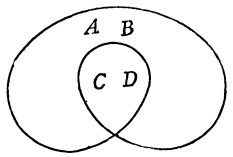
\includegraphics{scroll.png}
  \caption{Peirce's scroll}
  \labfig{scroll}
\end{marginfigure}

\reffig{scroll} shows Peirce's drawing of the scroll as it appears in
\cite[Fig.~5]{peirce_prolegomena_1906}. He defines its intended meaning like so
\cite[p.~534--535]{peirce_prolegomena_1906}:

\begin{quote}
  I shall call the outer boundary the Wall; and the inner, the Fence. In the
outer I scribed the Antecedent, in the inner the Consequent, of a Conditional
Proposition de inesse. [...][Thus the meaning of \reffig{scroll} is] that if
both A and B are true, then both C and D are true. [...] a Conditional de inesse
(unlike other conditionals) only asserts that either the antecedent is false or
the consequent is true. 
\end{quote}

This shows the classical view of Peirce on EG, who interprets the scroll as
signifying the \textit{conditional de inesse} --- also called nowadays
\emph{material implication}, and defined here in its disjunctive form, expressed
symbolically by $A \limp B \defeq \neg A \lor B$. This is no coincidence that
Peirce based his most fundamental icon on implication: according to Lewis
\sidecite[][p.~79]{Lewis1920-LEWASO-4}, he was the one who introduced the
``illative relation'' of implication into symbolic logic in the first place, by
giving it a distinguished symbol, and studying extensively the algebraic laws
that govern it (including Peirce's law).

\paragraph{Blank Antecedant}

\begin{marginfigure}
  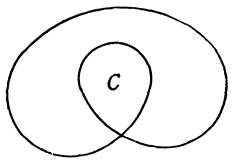
\includegraphics{empty-antecedant.png}
  \caption{Peirce's scroll with a blank antecedant}
  \labfig{empty-antecedant}
\end{marginfigure}

A first principle that Peirce derives from the scroll is the following
\cite[p.~534]{peirce_prolegomena_1906}:

\begin{quote}
  [...] any insertion [is] permitted in the outer close, and any omission from
the inner close. By applying the former clause of this rule to
[\reffig{empty-antecedant}], we see that this scroll with the outer close void,
justifies the assertion that if no matter what be true, C is in any case true;
so that the two walls of the scroll, when nothing is between them, fall
together, collapse, disappear, and leave only the contents of the inner close
standing, asserted, in the open field.
\end{quote}

This first form of ``collapsing of walls'' is called the \emph{Rule of Blank
Antecedant} in \cite{minghui_graphical_2019}, and corresponds symbolically to
the equivalence $\top \limp A \semequiv A$. The reader might be tempted to see
the ``former clause'' that permits any insertion in the outer close as a special
case of the Insertion principle of \sys{Alpha} (\refsec{alpha}). However, we
stress again that Peirce first identified this clause as a feature of the
scroll, seen as the diagrammatic embodiment of the ``general form of argument''
mentioned in a previous excerpt. The principle of Insertion only followed as a
subsequent generalization, stemming from the analysis of the scroll into two
nested cuts \cite[p.~535]{peirce_prolegomena_1906}:

\begin{quote}
  [...] and you will further see that a scroll is really nothing but one oval
within another.
\end{quote}

\begin{marginfigure}
  $$
  \!\!\!\!\stkfig{1}{scroll-empty-antecedant}
  \!\!\!\!\xinvstep{\rsf{BA}}~~~~
  G
  $$
  \caption{The rule of Blank Antecedant}
  \labfig{rule-empty-antecedant}
\end{marginfigure}

To emphasize this point, we will from now on depict scrolls as two nested cuts
joined at a single point highlighted in orange, as illustrated in
\reffig{rule-empty-antecedant}.

\begin{remark}
  It is interesting to note that the rule of Blank Antecedant is not seen as
  primitive by Peirce, but as a consequence of a \emph{dynamic potential} of the
  scroll: namely, the ability to insert anything in the outer close, at will.
  This is another manifestation of Peirce's concern for the question of
  \emph{illative atomicity}, and is to be related to the elimination of the
  Double-cut rule discussed in \refsec{atomicity}.
\end{remark}

\paragraph{Currying}

\begin{marginfigure}[-10em]
  ~~~\stkfig{0.8}{scroll-curried}
  \caption{Currying as scroll nesting}
  \labfig{scroll-curried}
\end{marginfigure}

\begin{marginfigure}[0em]
  \setlength{\fboxsep}{2pt}
\setlength{\arraycolsep}{0pt}
\newcommand{\vsp}{\vspace{-0.5em}}
\newcommand{\stkf}{\tikzfig{0.9}{0.5}}
$$
\begin{array}{r@{\quad}c@{\vsp}}
                                  &\stkf{eg-currying-3} \\
       \xstep{\kl{BA}} &\stkf{eg-uncurrying-1} \\
       \xstep{\kl{Ins}} &\stkf{eg-uncurrying-2} \\
       \xstep{\kl{Deit}} &\stkf{eg-currying-0}
\end{array}
$$
  \caption{Intuitionistic proof of currying}
  \labfig{eg-currying}
\end{marginfigure}

\begin{marginfigure}[27em]
  \setlength{\fboxsep}{2pt}
\setlength{\arraycolsep}{0pt}
\newcommand{\vsp}{\vspace{-0.5em}}
\newcommand{\stkf}{\tikzfig{0.9}{0.5}}
$$
\begin{array}{r@{\quad}c@{\vsp}}
                                  &\stkf{eg-currying-0} \\
       \xstep{\mathsf{Ins}} &\stkf{eg-currying-1} \\
       \xstep{\mathsf{Deit}} &\stkf{eg-currying-2} \\
       \xstep{\mathsf{BA}} &\stkf{eg-currying-3}
\end{array}
$$

  \caption{Intuitionistic proof of uncurrying}
  \labfig{eg-uncurrying}
\end{marginfigure}

Peirce was aware of the phenomenon of \emph{currying}, expressed symbolically by
the equivalence $A \limp B \limp C \semequiv A \land B \limp C$, as witnessed by
the following passage \cite[p.~535]{peirce_prolegomena_1906}:
\begin{quote}
Now, Reader, if you will just take pencil and paper and scribe the scroll
expressing that if $A$ be true, then it is true that if $B$ be true $C$ and $D$
are true [\reffig{scroll-curried}], and compare this with [\reffig{scroll}],
which amounts to the same thing in meaning, you will see that scroll walls with
a void between them collapse even when they belong to different scrolls.
\end{quote}
It is remarkable that he comes to this conclusion by a topological argument,
noting that this second form of ``collapsing of walls'', now involving two
different scrolls, follows from the scroll beeing composed of two nested cuts.
If we reject this interpretation by requiring that the Fence (the inner oval)
stays glued to the Wall (the outer oval), then one cannot derive currying
through the rule of double-cut, precisely because the system only permits to
collapse a Wall and a Fence continuously joined in the same scroll, by the
weaker rule of Blank Antecedant. Fear not however, as one can still derive the
currying and uncurrying laws in this intuitionistic setting, but through the
additional use of the insertion and deiteration rules, as depicted in
\reffig{eg-currying} and \reffig{eg-uncurrying}. Yet we find that Peirce's insight
on the topological explanation of currying in the classical setting remains
noteworthy.

\begin{remark}
Note that in \reffig{eg-currying} and \reffig{eg-uncurrying}, we give
\emph{direct} proofs that rewrite the premiss of the argument into its
conclusion, rather than \emph{goal-directed} proofs (\refdef{eg-proof}) that
rewrite a goal into the empty $\SA$, as we usually did in \refch{eg}. Direct
proofs are closer to Peirce's usage of the illative transformations --- and thus
to what can be found in most of the literature on EG, and have the advantage of
being more economical in space by leaving the goal implicit. One can easily go
from a direct proof to a goal-directed one as shown by the \emph{deduction
theorem} of Sowa \cite[Section 6]{sowa_peirces_2011}, which also applies
in the intuitionistic setting by substituting the rule of Double-cut with the
rule of Blank Antecedant.
\end{remark}

\paragraph{The $n$-ary scroll}

In \cite{oostra_graficos_2010}, A. Oostra proposes to take the above remark
seriously, by reifying the scroll as a primitive icon of EG (``\emph{rizo}'' in
Spanish), that exists alongside the cut (``\emph{corte}''), and is distinguished
from it. In fact he goes further than this, and proposes to generalize both the
cut and the scroll into an $n$-ary construction called the \emph{curl}
(``\emph{bucle}''), where $n$ is the number of inner closes, called \emph{loops}
(``\emph{lazos}''). \reffig{five-loops} shows an example of curl with five
loops. In \cite{minghui_graphical_2019}, the curl is simply called \emph{$n$-ary
scroll}, and is analyzed into the outer area (that enclosed by the Wall) called
the \emph{outloop}, and the inner areas (those enclosed by the $n$ Fences, i.e.
the loops of Oostra) called the \emph{inloops}. Then cuts and scrolls are indeed
special cases of $n$-ary scrolls, respectively with $n = 0$ and $n = 1$.

\begin{marginfigure}
  \stkfig{1}{five-loops}
  \caption{A curl with five loops}
  \labfig{five-loops}
\end{marginfigure}

Like the unary scroll, the $n$-ary scroll is to be read as an implication whose
antecedant is the content of the outloop, and consequent the content of the
inloops. The generalization then consists in taking the \emph{disjunction} of
the contents of all inloops: this reflects nicely the etymological meaning of
the word ``disjunction'', since the inloops enclose \emph{disjoint} areas of the
outloop to which they are attached. Then the $5$-ary scroll of
\reffig{five-loops} is read as the formula $a \limp b \lor c \lor d \lor e \lor
f$; and the $0$-ary scroll obtained by removing all inloops from the latter as
$a \limp \bot$, since a $0$-ary disjunction is naturally evaluated to its
neutral element $\bot$. This coincides with the intuitionistic reading of
negation $\neg A \defeq A \limp \bot$, and is thus consistent with the
interpretation of cuts as negations.

\paragraph{Continuity}

\begin{marginfigure}
  $$
\begin{array}{c}
  \begin{array}{cc}
    \stkfig{1}{scroll-disj} & A \lor B \\
    \stkfig{1}{scroll-imp} & A \limp B \\[1em]
    \multicolumn{2}{c}{\not=} \\
    \stkfig{1}{eg-disj} & \neg (\neg A \land \neg B) \\
    \stkfig{1}{eg-imp} & \neg (A \land \neg B)
  \end{array}
\end{array}
$$
  \caption{Continuity, disjunction and implication in IEG}
  \labfig{eg-disj-imp}
\end{marginfigure}

With this interpretation of the $n$-ary scroll, the \sys{Alpha} encodings of
disjunction and implication as nested cuts are no longer valid, because they are
not intuitionistically equivalent to the associated binary and unary scrolls.
This is illustrated in \reffig{eg-disj-imp}, where the closeness in meaning is
reflected iconically (but not symbolically) in the fact that the graphs only
differ in the \emph{continuity} (or lack thereof) between inloops and their
outloop. Indeed, contrary to nested cuts, any $n$-ary scroll can be drawn by a
\emph{continuous} movement of the pen, producing a self-intersecting curve as
described by Peirce in \cite{peirce_prolegomena_1906}. This might be related to
other manifestations of the notion of continuity in the semantics of
intuitionistic logic, such as the well-known Stone-Tarski interpretation of
formulas as topological spaces \cite{stone_topological_1938}, and the
interpretation of proofs as continuous maps in the \emph{denotational semantics}
of Dana Scott \sidecite{10.5555/218742.218744}. Before the advent of Oostra's
IEG, Zalamea gave a detailed analysis of Peirce's philosophy of
the \emph{continuum}, how it relates to modern developments in mathematics, and
how it is embodied in existential graphs \cite{zalamea_peirces_2003}. Actually
according to Oostra \sidecite[][p.~162]{oostra_advances_2022}, ``the
possibility of developing intuitionistic existential graphs was first suggested
by Zalamea in the 1990s \cite{zalamea_ieg_1}\cite{zalamea_ieg_2}''.

\paragraph{Coherent formulas}

\begin{marginfigure}
  $$
  \!\!\!\!
  \!\!\!\!
  \!\!\!\!
  \begin{array}{c}
    \tikzfig{0.85}{0.85}{curl-geom} \vspace{1.5em}\\
    \forall \bx. \left(\bigwedge G \limp \bigvee_{j = 1}^{n}\exists \bx_j. \bigwedge H_j\right)
  \end{array}
  $$
  \caption{Formula interpretation of the $n$-ary scroll}
  \labfig{curl-geom}
\end{marginfigure}

More generally, a $n$-ary scroll with atoms $G \deq a_1, \ldots, a_m$ in its
outloop and $\Delta \deq \begin{pmatrix} a_{1,1} & \ldots & a_{1,p_1} \\
  \vdots & \ddots & \vdots \\
  a_{n,1} & \ldots & a_{1,p_n}
\end{pmatrix}$
in its inloops, where each row $H_j$ in $\Delta$ encodes an inloop, can be
interpreted as the formula
$$\bigwedge_{i = 1}^{m}{a_i} \limp \bigvee_{j = 1}^{n}\bigwedge_{k = 1}^{p_n}{a_{j,k}}$$
If one adds \emph{binders} to the mix (see \refsec{gardens}) by having $\gamma \deq
\garden{\bx}{G}$ as outloop, and
$\Xi \deq \begin{pmatrix}
  \bx_1 \\
  \vdots \\
  \bx_n
\end{pmatrix} \cdot \Delta$ as inloops, then the interpretation is extended into
the formula
$$\forall \bx. \left(\bigwedge_{i = 1}^{m}{a_i} \limp \bigvee_{j = 1}^{n}\exists \bx_j. \bigwedge_{k = 1}^{p_n}{a_{j,k}}\right)$$
as depicted in \reffig{curl-geom}. Typically, the particular case where $\gamma
\deq \garden{x}{\emptyset}$ and $\Xi \deq (\emptyset) \cdot (p(x))$ encodes the graph
$$\stkfig{1}{scroll-forall}$$
expressing the universal quantification $\forall x. p(x)$, and the case where
$\gamma \deq \garden{\emptyset}{\emptyset}$ and $\Xi \deq (x) \cdot (p(x))$ the graph
$$\stkfig{1}{scroll-exists}$$
expressing the existential quantification $\exists x. p(x)$. The interpretation
is invariant under polarity, meaning that for instance the graphs
$$\stkfig{1}{scroll-neg-forall} \text{   and   } \stkfig{1}{scroll-neg-exists}$$
obtained by enclosing the previous graphs in a cut are interpreted with the same
quantifiers, as the formulas $\neg \forall x. p(x)$ and $\neg \exists x. p(x)$.
In \sys{Beta}, we would have exploited the classical equivalences $\neg \forall
x. A \semequiv \exists x. \neg A$ and $\neg \exists x. A \semequiv \forall x.
\neg A$ (justified by the double-cut principle) in order to interpret them as
$\exists x. \neg p(x)$ and $\forall x. \neg p(x)$, emphasizing the idea that
positive and negative binders encode respectively $\exists$ and $\forall$. But
this is not possible anymore with the intuitionistic interpretation of $n$-ary
scrolls, where the $\exists/\forall$ duality is replaced by the inloop/outloop
distinction. In fact, we are tempted to further qualify this distinction of
\emph{adjunction}, following a classical result of Lawvere in the context of
categorical logic \sidecite{lawvere_quantifiers_sheaves}.

Lawvere is also known for some contributions to the study of \emph{geometric
logic} \sidecite{lawvere_geometric}, a subset of the formulas of FOL first
discovered by Skolem \sidecite{skolem_geometric} that is capable of expressing
many mathematical theories, and has close connections to \emph{topos theory}.
Quite remarkably, the interpretation of $n$-ary scrolls coincides exactly with
the class of \emph{coherent formulas}, which are the formulas of geometric logic
where infinitary disjunctions are restricted to finitary ones. There is a
difference however: the full syntax of IEG allows for arbitrary \emph{nestings}
of $n$-ary scrolls inside eachother, i.e. the multisets $G$ and $H_j$ in
\reffig{curl-geom} can contain $n$-ary scrolls in addition to atoms; while
coherent formulas are restricted to atoms.

Coherent formulas have some nice properties, which might also apply to IEG to
some extent. We only mention two important ones:
\begin{description}
  \item[Completeness] Every first-order theory has a coherent conservative
  extension, making coherent formulas (and thus non-nested $n$-ary scrolls) in
  principle as expressive as arbitrary first-order formulas
  \sidecite{negri_geometric}.
  
  \item[Automation] Coherent formulas benefit from faster proof-search
  procedures compared to arbitrary formulas, making automation more tractable
  computationally. They also allow the direct encoding of many reasoning
  problems, thanks to their use of the full set of connectives and quantifiers
  of FOL; and avoiding complex encodings (as can be found e.g. in SMT solvers)
  is crucial in \emph{interactive} theorem proving, where the user and the
  computer manipulate the same formulas in goals
  \sidecite{bezem_automating_2005}. This has been exploited already in some
  domain-specific theorem provers, like the Larus prover that automatically
  generates illustrated proofs in geometry\sidenote{Incidentally, projective
  geometry was one of the motivating applications that led Skolem to identify
  the class of coherent formulas \cite{bezem_automating_2005}.}
  \sidecite{narboux_larus}.
  
  \begin{remark}
  Thus with IEG, one becomes able to reason \emph{geometrically} on geometric
  formulas that speak about geometry: another beautiful incarnation of the
  reflexivity at work in Peirce's iconic logic.
  \end{remark}
\end{description}

\section{Flowers}\labsec{Flowers}

\paragraph{Blooming}

As we have seen, the ($n$-ary) scroll is a powerful icon, because it captures
the distinction between classical and intuitionistic logic as being a matter of
\emph{continuity} between the space of inputs/hypotheses (outloop) and the
spaces of outputs/conclusions (inloops), reflecting an intuition discovered much
later in the denotational semantics of the $\lambda$-calculus. However as a
diagrammatic component to be operated upon through direct manipulation, it has
one notable flaw, also shared with the classical cut-based syntax: it quickly
induces heavy nestings of curves in the plane, making even a simple graph like
that of \reffig{scroll-curried} hard to read for an untrained eye.

\begin{marginfigure}
  $$
  \tikzfig{1}{0.4}{scroll-inside-out}
  $$
  \caption{Turning a $5$-ary scroll inside-out}
  \labfig{scroll-inside-out}
\end{marginfigure}

Before devising an alternative syntax, one should ask: what are the essential
features of the scroll that we want to preserve? Following the previous
observations, we identified two of them:
\begin{itemize}
  \item[\textbf{Continuity}] the scroll is a self-intersecting continuous curve,
  which can be drawn in one stroke of the pen;
  \item[\textbf{Polarity}] this curve delineates two kinds of areas: inloops that have
  the same polarity as the area on which the scroll is scribed, and the outloop
  which has the opposite polarity.
\end{itemize}

Fortunately, these two properties are preserved when turning inloops
\emph{inside-out}, as illustrated in \reffig{scroll-inside-out}. This might be
because the very process of turning inside-out can be seen as a continuous
movement in three-dimensional space, where the inloops are rotated around their
intersection points with the outloop. In this way, we have effectively divided
the amount of curve-nesting in scrolls by two. And as an added bonus, the new
icon is reminiscent of a \emph{flower}, as if it had bloomed from its curled
bud; or as if the pistol cylinder from \reffig{five-loops} had transformed into
a \emph{pistil}, and its bullet chambers into \emph{petals}\sidenote{As the
saying goes: make love, not war.}.

\begin{marginfigure}
  $$
  \!\!\!\!
  \!\!\!\!
  \!\!\!\!
  \!\!\!\!
  \stkfig{0.65}{flowers}
  $$
  \vspace{-3em}
  \caption{Nested flowers}
  \labfig{flowers}
\end{marginfigure}

From that point onwards, we decided to fully embrace the flower metaphor: first
in our drawing style as witnessed in \reffig{flowers}, but also in our syntactic
terminology, to be introduced in the next pages. Negative outloops are now drawn
as \emph{yellow} pistils for a more colorful experience, and inloops as
transparent petals, i.e. of the same color as the area on which they are
scribed. We also drop the requirement that petals should intersect their pistil
at a single point, for purely aesthetic reasons.

\paragraph{Multisets}

As we did for classical EG in \refsec{multisets} and \refsec{gardens}, we are
now going to distill the syntactic essence of flowers into an inductive,
(multi)set-based data structure. This will allow for a more compact textual
notation, that is better suited to proof-theoretical study.

In \refsec{beta}, we explained how the graphs of \sys{Beta} allow to represent
purely relational statements, without function symbols. Since functions are just
deterministic relations, one can in principle formalize any first-order theory
in this syntax\sidenote{Conversely, every relation can be faithfully encoded as
its characteristic function, which is the basis for the formalization of
mathematics in \emph{type theories}.}. However it is much more convenient to
have a dedicated syntax for functions, and we will thus introduce them as is
usually done in predicate calculus.

\begin{definition}[First-order signature]
  A \emph{first-order signature} is a triplet $\mathcal{\Sigma} = (
  \fsymbs, \psymbs, \arity )$, where $\fsymbs$ and $\psymbs$ are
  respectively the countable sets of \emph{function} and \emph{predicate}
  symbols of $\Sigma$, and $\arity : \fsymbs \cup \psymbs \to \nats$ gives an
  \emph{arity} to each symbol.
\end{definition}

In the following, we assume given a denumerable set of variables $\vars$
and a first-order signature $\Sigma$.

\begin{definition}[Terms]
  The set of terms $\terms$ is defined inductively as follows:
  \begin{itemize}
    \item{\textbf{(Variable)}} If $x \in \vars$ then $x \in \terms$;
    \item{\textbf{(Application)}} If $f \in \fsymbs$ and $\tvec{t}
    \in \terms^{\arity(f)}$, then $f(\tvec{t}) \in \terms$.
  \end{itemize}
\end{definition}

\begin{definition}[Flowers]\labdef{flowers}
  The sets of \emph{flowers} $\flowers$ and \emph{gardens} $\gardens$ are
  defined mutually inductively as follows:
  \begin{itemize}
    \item{\textbf{(Atom)}} If $p \in \psymbs$ and $\tvec{t} \in
    \terms^{\arity(p)}$, then $p(\tvec{t}) \in \flowers$;
    \item{\textbf{(Garden)}} If $\bx \subset \vars$ is a finite set and $\Phi
    \subset \flowers$ a finite multiset, then $\garden{\bx}{\Phi} \in
    \gardens$;
    \item{\textbf{(Flower)}} If $\gamma \in \gardens$ and $\Delta \subset \gardens$
    is a finite multiset, then $\flower{\gamma}{\Delta} \in \flowers$.
  \end{itemize}
\end{definition}

Any finite set $\bx \subset \vars$ of variables is called a \emph{sprinkler},
finite multiset $\Phi \subset \flowers$ of flowers a \emph{bouquet}, and finite
multiset $\Gamma \subset \gardens$ of gardens a \emph{corolla}. We will often
write gardens as $\garden{x_1, \ldots, x_n}{\phi_1, \ldots, \phi_m}$, where the
$x_i$ are called \emph{binders}; and non-atomic flowers as
$\flower{\gamma}{\delta_1 \sep \ldots \sep \delta_n}$, where $\gamma$ is the
\emph{pistil}, and the $\delta_i$ are called \emph{petals}. We write
$\fset{i}{n}{E_i}$ to denote a finite (multi)set of size $n$ with elements $E_i$
indexed by $1 \leq i \leq n$. We also omit writing the empty (multi)set,
accounting for it with blank space as is done in sequent notation or in EG; in
particular, $\garden{{}}{{}}$ stands for the empty garden
$\garden{\emptyset}{\emptyset}$, $\flower{\gamma}{{}}$ for the flower with no
petals $\flower{\gamma}{\emptyset}$, and $\flower{\gamma}{\garden{{}}{{}}}$ for
the flower with one empty petal.

Note that the order of precedence of operators is
$\mathop{,} < \garden{{}}{{}} < \mathop{;} < \mathop{\flower{}{}}$
so that for instance, the string
$$\flower{\garden{x_1, x_2}{\phi_1, \phi_2}}{\garden{y_1}{\psi, (\flower{\gamma}{\Delta})} \sep \garden{y_2}{\Phi}}$$
is parsed as the flower
% $$\left(\flower{\left(\garden{\{x_1, x_2\}}{\{\phi_1,
% \phi_2\}}\right)}{\{\left(\garden{\{y_1\}}{\{\psi,
% \left(\flower{\gamma}{\Delta}\right)\}}\right) \sep
% \left(\garden{\{y_2\}}{\Phi}\right)\}}\right)$$ where constructed finite
% (multi)sets are delimited with $\{\}$, and constructed flowers/gardens are
% delimited with $()$.
\vspace{-6em}
$$\stkfig{1}{parsed-flower}$$
\vspace{-6em}

Also to improve readability, we will most of the time omit the garden dot
`$\cdot$' when the sprinkler is empty, writing $\Phi$ instead of
$\garden{{}}{\Phi}$.

\begin{remark}
  In some places the choice of letter for meta-variables will be important to
  disambiguate the kind of syntactic object we denote. \reftab{letters}
  summarizes our chosen notational conventions in this respect.
\end{remark}

\begin{marginfigure}
  \centering
  \begin{tabular}{|c|c|}
    \hline
    \bfseries Kind & \bfseries Letters \\
    \hline
    Variables ($\vars$) & $x, y, z$ \\
    Terms ($\terms$) & $t, u, v$ \\
    Flowers ($\flowers$) & $\phi, \psi, \xi$ \\
    Gardens ($\gardens$) & $\gamma, \delta$ \\
    Sprinklers & $\bx, \by, \bz$ \\
    Term vectors & $\tvec{t}, \tvec{u}, \tvec{v}$ \\
    Substitutions & $\sigma, \tau$ \\
    Bouquets & $\Phi, \Psi, \Xi$ \\
    Corollas & $\Gamma, \Delta$ \\
    Contexts & $\Phi\hole, \Psi\hole, \Xi\hole$ \\
    Theories & $\mathcall{T}, \mathcall{U}$ \\
    \hline
  \end{tabular}
  \caption{Notational conventions for meta-variables}
  \labtab{letters}
\end{marginfigure}

As usual, we introduce a \emph{depth} measure that will allow us to reason
inductively on the structure of flowers:
\begin{definition}[Depth]
  The \emph{depth} $\soldepth{-}$ of a flower or garden is defined mutually
  recursively as follows:
  \begin{align*}
    \soldepth{p(\tvec{t})} &= 0 \\
    \soldepth{\garden{\bx}{\Phi}} &= \max_{\phi \in \Phi}{\soldepth{\phi}} \\
    \soldepth{\flower{\gamma}{\Delta}} &= 1 + \max(\soldepth{\gamma}, \max_{\delta \in \Delta}{\soldepth{\delta}})
  \end{align*}
\end{definition}

We now proceed with routine definitions for handling variables and substitutions
of terms in flowers.

\begin{definition}[Free variables]\labdef{fv}
  
  The sets of \emph{free variables} $\fv(-)$ of a term, flower, bouquet or
  garden are defined mutually recursively as follows:
  \begin{align*}
    \fv(x) &= \{x\} &
    \fv(\Phi) &= \bigcup_{\phi \in \Phi}{\fv(\phi)} \\
    \fv(f(\tvec{t})) &= \bigcup_{t \in \tvec{t}}{\fv(t)} &
    \fv(\garden{\bx}{\Phi}) &= \fv(\Phi) \setminus \bx \\
    \fv(p(\tvec{t})) &= \bigcup_{t \in \tvec{t}}{\fv(t)} &
    \fv(\flower{\garden{\bx}{\Phi}}{\Delta}) &= \fv(\garden{\bx}{\Phi}) \cup \bigcup_{\garden{\by}{\Psi} \in \Delta}{\fv(\garden{\bx, \by}{\Psi})}
  \end{align*}
  We say that a term, flower, bouquet or garden is \emph{closed} when its set of
  free variables is empty.
  % The sets of closed terms, flowers and gardens are denoted respectively by
  % $\closed{\terms}$, $\closed{\flowers}$ and $\closed{\gardens}$.
\end{definition}

\begin{remark}\labremark{flower-scope}
Note that the scope of a binder located in a pistil extends both to the pistil
\emph{and} to all its attached petals, whereas for a binder located in a petal
it is limited to said petal. This is reflected in the above definition of free
variables for (non-atomic) flowers, and is visually explained by the nesting of
curves in an $n$-ary scroll.
\end{remark}

\begin{definition}[Bound variables]
  % The set of \emph{bound variables} $\bv(\Phi\hole)$ of a context $\Phi\hole$ is defined
  % inductively as follows:
  % \begin{align*}
  %   \bv(\Psi, \hole) &= \emptyset \\
  %   \bv(\Psi, (\flower{\garden{\bx}{X}}{\Delta})) &= \bx \cup \bv(X) \\
  %   \bv(\Psi, (\flower{\garden{\bx}{\Phi}}{\garden{\by}{X} \sep \Delta})) &= \bx \cup \by \cup \bv(X)
  % \end{align*}
  The sets of bound variables $\bv(-)$ of a flower, bouquet or garden are
  defined mutually recursively as follows:
  \begin{align*}
    \bv(p(\tvec{t})) &= \emptyset &
    \bv(\garden{\bx}{\Phi}) &= \bx \cup \bv(\Phi) \\
    \bv(\Phi) &= \bigcup_{\phi \in \Phi}{\bv(\phi)} &
    \bv(\flower{\gamma}{\Delta}) &= \bv(\gamma) \cup \bigcup_{\delta \in \Delta}{\bv(\delta)}
  \end{align*}
\end{definition}

To avoid reasoning about $\alpha$-equivalence, we adopt in this work the
so-called \emph{Barendregt convention} that all variable binders are distinct,
both among themselves and from eventual free variables. Formally, we assume that
for any bouquet $\Phi$, the two following conditions hold:
\begin{enumerate}
  \item computing $\bv(\Phi)$ as a multiset gives the same result as computing
  it as a set;
  \item $\bv(\Phi) \cap \fv(\Phi) = \emptyset$.
\end{enumerate} 
% To preserve this convention, in this paper we will only consider
% \emph{non-circular} substitutions $\sigma$ where $x \not\in \fv(\sigma(x))$ for
% all $x \in \dom(\sigma)$.

To define substitutions, we introduce a general notion of \emph{function
update}, which will be useful for the semantic evaluation of flowers in
\refsec{Semantics}.

\begin{definition}[Function update]
  Let $A, B$ be two sets, $f, g : A \to B$ two functions and $R \subseteq A$
  some subset of their domain. The \emph{update} of $f$ on $R$ with $g$ is the
  function defined by:
  $$
  (\update{f}{R}{g})(x) =
  \begin{cases}
    g(x) &\text{if $x \in R$} \\
    f(x) &\text{otherwise}
  \end{cases}
  $$
  $\update{-}{-}{-}$ is left-associative, that is
  $\update{f}{R}{\update{g}{S}{h}} = \update{(\update{f}{R}{g})}{S}{h}$. Also
  if $f$ or $g$ is the identity function $\idsubst$ we omit writing it, i.e.
  $\update{f}{R}{{}} = \update{f}{R}{\idsubst}$ and $\update{{}}{R}{g} =
  \update{\idsubst}{R}{g}$.
\end{definition}

\begin{fact}[Associativity]\labfact{update-assoc}
  $\update{\update{f}{R}{g}}{S}{h} = \update{f}{R \cup S}{(\update{g}{S}{h})}$.
\end{fact}

\begin{fact}[Commutativity]\labfact{update-comm}
  If $R \cap S = \emptyset$ then $f \upd{R} g \upd{S} h = f \upd{S} h \upd{R}
  g$.
\end{fact}

\begin{fact}[Agreement]\labfact{update-agree}
  If $f(x) = g(x)$ for all $x \in R$ then $h \upd{R} f = h \upd{R} g$.
\end{fact}

\begin{fact}[Idempotency]\labfact{update-idempot}
  $f \upd{R} f = f$.
\end{fact}

\begin{definition}[Substitution]
  A \emph{substitution} is a function $\sigma : \vars \to \terms$ with a finite
  \emph{support} $\dom(\sigma) = \compr{x}{\sigma(x) \not= x}$. By abuse of
  notation, we will write $\sigma : \bx \to \terms$ to denote a substitution
  $\sigma$ whose support is $\bx$. The domain of substitutions is extended to
  terms, flowers, bouquets and gardens mutually recursively as follows:
  \begin{align*}
    \sigma(f(t_1, \ldots, t_n)) &= f(\sigma(t_1), \ldots, \sigma(t_n)) \\
    \sigma(p(t_1, \ldots, t_n)) &= p(\sigma(t_1), \ldots, \sigma(t_n)) \\
    \sigma(\phi_1, \ldots, \phi_n) &= \sigma(\phi_1), \ldots, \sigma(\phi_n) \\
    \sigma(\garden{\mathbf{x}}{\Phi}) &=
      \garden{\mathbf{x}}{\restr{\sigma}{\mathbf{x}}(\Phi)} \\
    \sigma(\flower{\garden{\mathbf{x}}{\Phi}}{\delta_1 \sep \ldots \sep \delta_n}) &=
      \flower{\sigma(\garden{\mathbf{x}}{\Phi})}{\restr{\sigma}{\mathbf{x}}(\delta_1) \sep \ldots \sep \restr{\sigma}{\mathbf{x}}(\delta_n)}
  \end{align*}

\end{definition}

\begin{definition}[Capture-avoiding substitution]
  We say that a substitution $\sigma : \bx \to \terms$ is
  \emph{capture-avoiding} in a bouquet $\Phi$ if $\fv(\sigma(x)) \cap \bv(\Phi)
  = \emptyset$ for every $x \in \bx$.
  % $\fv(\sigma(x)) \cap \bv(\phi) = \emptyset$ for every $x \in
  % \bx$, or $\bx \cap \fv(\phi) = \emptyset$.
  % \begin{itemize}
  %   \item $\phi = p(\tvec{t})$;
  %   \item $\phi =
  %   \flower{\garden{\by}{\Phi}}{\fset{i}{n}{\garden{\bz_i}{\Psi_i}}}$,
  %   $\fv(\sigma(x)) \cap \left(\by \cup \bigcup_{i = 1}^{n}{\bz_i}\right) =
  %   \emptyset$ for every $x \in \bx \cap \left(\fv(\Phi) \cup \bigcup_{i =
  %   1}^{n}{\fv(\Psi_i)}\right)$, and $\sigma$ is capture-avoiding in $\Phi \cup
  %   \bigcup_{i = 1}^{n}{\Psi_i}$.
  %   % \item $\bx \cap \fv(\phi) = \emptyset$.
  % \end{itemize}
\end{definition}

\section{Calculus}\labsec{Calculus}

\paragraph{Contexts}

Equipped with an inductive syntax, we can now express formally the inference
rules of our flower calculus, just as we did for \sys{Alpha}
(\refsec{multisets}) and \sys{Beta} (\refsec{gardens}). There, graphs and their
contexts were defined as multisets of nodes, which have now turned into bouquets
of flowers:

\begin{definition}[Context]
  A \emph{bouquet context} $\Phi\hole$ is a bouquet which contains exactly one
  occurrence of the special flower $\hole$ called the \emph{hole}. The hole can
  always be \emph{filled} (substituted) with any other bouquet $\Psi$ or context
  $\Xi\hole$, producing a new bouquet $\cfill{\Phi}{\Psi}$ or context
  $\cfill{\Phi}{\Xi\hole}$. In particular, filling with the empty bouquet will
  yield a bouquet $\cfill{\Phi}{\phantom{\Phi}}$, which is just $\Phi\hole$ with
  its hole removed. A \emph{flower context} $\phi\hole$ is a bouquet context of
  size $1$.
\end{definition}

\begin{definition}[Depth]
  The \emph{depth} $\soldepth{\Phi\hole}$ of a bouquet context $\Phi\hole$ is
  defined recursively as follows:
  \begin{align*}
    \soldepth{\Psi, \hole} &= 0 \\
    \soldepth{\Psi, (\flower{\garden{\bx}{\Phi\hole}}{\Delta})} &= 1 + \soldepth{\Phi\hole} \\
    \soldepth{\Psi, (\flower{\gamma}{\garden{\bx}{\Phi\hole} \sep \Delta})} &= 1 + \soldepth{\Phi\hole}
  \end{align*}
\end{definition}

Contrarily to EG (\refdef{eg-parity}), the parity of a context does not coincide
with its depth, since petals increase depth but preserve polarity:

\begin{definition}[Parity]
  The \emph{parity} $\parity{\Phi\hole}$ of a context $\Phi\hole$ is defined
  recursively by:
  \begin{align*}
    \parity{\Psi, \hole} &= 0 \\
    \parity{\Psi, (\flower{\garden{\bx}{\Phi\hole}}{\Delta})} &= \parity{\Phi\hole} + 1 \\
    \parity{\Psi, (\flower{\gamma}{\garden{\bx}{\Phi\hole} \sep \Delta})} &= \parity{\Phi\hole}
  \end{align*}
\end{definition}

\begin{definition}[Polarity]
  We say that a context $\Phi\hole$ is \emph{positive} if $\parity{\Phi\hole}$ is even, and
  \emph{negative} otherwise. We denote positive and negative contexts
  respectively by $\Phi^+\hole$ and $\Phi^-\hole$.
\end{definition}

\paragraph{Pollination}

In order to formulate the equivalent of the (de)iteration rules of EG for
flowers, we introduce a \emph{pollination} relation that captures the
availability of a flower in a given context, akin to the \emph{justification}
relation of \refsec{atomicity}:

\begin{definition}[Pollination]\labdef{pollination} We say that a flower $\phi$
  can be \emph{pollinated} in a context $\Phi\hole$, written
  $\chyp{\phi}{\Phi\hole}$, when there exists a bouquet $\Psi$ with $\phi \in
  \Psi$ and contexts $\Xi\hole$ and $\Xi_0\hole$ such that either:
  \begin{itemize}
    \item (\textbf{Cross-pollination})~ $\Phi\hole = \cfill{\Xi}{\Psi,
    \Xi_0\hole}$;
    \item (\textbf{Self-pollination})~ $\Phi\hole =
    \cfill{\Xi}{\flower{\garden{\bx}{\Psi}}{\garden{\by}{\Xi_0\hole}
    \sep \Delta}}$ for some $\bx, \by, \Delta$.
  \end{itemize}
  A bouquet $\Psi$ can be pollinated in $\Phi\hole$, written
  $\chyp{\Psi}{\Phi\hole}$, if $\chyp{\psi}{\Phi\hole}$ for all $\psi \in \Psi$.
\end{definition}

\begin{marginfigure}
  $$
  \!\!\!\!
  \!\!\!\!
  \!\!\!\!
  \begin{array}{c}
    \tikzfig{1}{0.5}{cross-pollination} \vspace{-2em} \\
    \text{\textit{Cross-pollination}} \vspace{-1em} \\
    \tikzfig{1}{0.5}{self-pollination} \vspace{-2em} \\
    \text{\textit{Self-pollination}}
  \end{array}
  $$
  \caption{Pollination in flowers}
  \labfig{pollination}
\end{marginfigure}

We now employ the metaphor of \emph{pollination} to speak about (de)iteration in
flowers. This is illustrated in \reffig{pollination}, where the blue dot marks
the location of the justifying/pollinating occurrence of $\phi$, and the red
dots all the areas that it (locally) justifies/pollinates, and thus where $\phi$
can be (de)iterated\sidenote{\reffig{pollination} summarizes visually the flow
of information in flowers, just like \reffig{eg-local-justification} summarized
the flow of information in EG, and \reffig{bubbles-porosity} in bubbles. From a
UI point of view, all these figures can be understood as kind of
``cheatsheets'', that indicate with arrows the allowed drag-and-drop moves for
importing a statement (the source of the DnD) into a new context (the
destination of the DnD).}. We distinguish two cases of \emph{cross}-pollination
and \emph{self}-pollination, as botanists do when describing the reproduction of
flowers. This distinction does not exist in classical EG, because pistils and
petals are both identified as instances of cuts\sidenote{The same phenomenon is
at work in \emph{subformula linking} (\refch{sfl}): self-pollination and
cross-pollination correspond respectively to the \emph{backward} $\back$ and
\emph{forward} $\forw$ linking operators, which are collapsed into a single
interaction operator $\ast$ in the original formulation of subformula linking
for classical linear logic \cite{Chaudhuri2013}.}. If we were to replace binders
by LoI (lines of identity, see \refsec{beta}), then the pollination relation
would also prescribe in which areas LoI can be extended/iterated, providing an
explanation for the scope of binders (\refremark{flower-scope}).

\paragraph{Rules}

As has become standard in this thesis, we define the flower calculus as a
\emph{rewriting system} on bouquets, presented in \reffig{flower-calculus} as a
set of unary deep inference rules: when read \emph{top-down}, they correspond to
usual inferences from premiss to conclusion, and will be justified by the
soundness theorem of \refsec{Soundness}.
% This gives them a \emph{static}, \emph{a posteriori} meaning, since this is
% typically how you would check the validity of an established inference
% \emph{after the fact}.
But the more interesting direction, and the one around which the calculus has
been designed, is when you read the rules \emph{bottom-up}: then they are indeed
rewrite rules, telling you the different ways in which you can choose to
simplify a goal. This is how the \emph{graphical} version of the rules is
presented in \reffig{natural-graphical} and \reffig{cultural-graphical}.
% Note that in the graphical presentation, the rules
% $\{\rsf{poll{\da}},\rsf{poll{\ua}},\rsf{grow},\rsf{crop}\}$ (resp.
% $\{\rsf{pull},\rsf{glue}\}$) manipulate a single flower (resp. petal) instead of
% an arbitrary bouquet $\Phi$ (resp. corolla $\Gamma$); but it is easy to see that
% these two variants are interderivable.

Let us now describe the rules in more detail, starting with the fragment that is
a direct adaptation of the rules of \sys{Beta} (\reffig{beta}):

\begin{description}
  \item[Blank Antecedant (\rsf{epis})]
    
    \begin{marginfigure}
      $$
      \R[\rsf{epis{\da}}]
        {\Phi}
        {\flower{\garden{{}}{{}}}{\garden{{}}{\Phi}}}
      $$
      \caption{Converse of \rsf{epis} rule}
      \labfig{flowers-episda}
    \end{marginfigure}

    It allows to enclose any bouquet in a petal attached to an \textsf{(e)}mpty
    \textsf{(pis)}til. This is one direction of the rule \rsf{BA} of
    (\reffig{rule-empty-antecedant}), which is a weaker, intuitionistic version
    of the classical rule \rsf{Dcut{\ua}} of \sys{Alpha} and \sys{Beta}. The
    other direction (rule \rsf{epis{\da}} in \reffig{flowers-episda}) is
    actually admissible, which might be related to the co-admissibility of
    \rsf{Dcut{\da}} in \sys{Alpha} (Corollary \ref{cor:adm-ins}).
  % \item[Blank Antecedant (\rsf{epis{\ua}}, \rsf{epis{\da}})]
  %   They allow to enclose (\rsf{epis{\ua}}) or free (\rsf{epis{\da}}) any
  %   bouquet in a petal attached to an \textsf{(e)}mpty \textsf{(pis)}til. They
  %   correspond to the rule \rsf{BA} of \reffig{rule-empty-antecedant}, which is
  %   a weaker, intuitionistic version of the classical rules \rsf{Dcut{\ua}} and
  %   \rsf{Dcut{\da}} of \sys{Alpha} and \sys{Beta}. \rsf{epis{\da}} will be shown
  %   to be admissible in \refsec{Completeness}, which might be related to the
  %   co-admissibility of \rsf{Dcut{\da}} in \sys{Alpha} (Corollary
  %   \ref{cor:adm-ins}).

  \item[(De)iteration (\rsf{poll{\da}}, \rsf{poll{\ua}})]
    Renamed \emph{\textsf{(poll)}ination} rules, they correspond to the rules
    \rsf{Iter} and \rsf{Deit} of \sys{Alpha} and \sys{Beta}, but reformulated
    with the pollination relation (\refdef{pollination}). In fact in their
    textual presentation of \reffig{flower-calculus}, they are more general than
    (de)iteration rules, because \refdef{pollination} allows the pollinating
    bouquet $\Phi$ to be \emph{scattered} in the context $\Xi\hole$, i.e. its
    flowers need not be located in the same area. On the contrary in the
    graphical presentation of \reffig{natural-graphical}, they are less general
    since only one flower can be pollinated at a time, rather than an entire
    bouquet of flowers residing in the same area. But it is easy to see that all
    these variants are equivalent in deductive power, since the pollination of a
    bouquet (however scattered) can always be simulated by the successive
    pollinations of each of its flowers.

  \item[Insertion/Deletion (\rsf{grow}, \rsf{crop}, \rsf{pull}, \rsf{glue})]
    They correspond to the rules \rsf{Ins} and \rsf{Del} of \sys{Alpha} and
    \sys{Beta}, but have doubled in number to account for the syntactic
    distinction between pistils and petals. More precisely, rules \rsf{grow} and
    \rsf{crop} allow to insert and delete entire flowers, while rules \rsf{pull}
    and \rsf{glue} deal with petals. As for pollination rules, manipulating
    single flowers/petals (graphical version) or entire bouquets/corollas
    (textual version) does not change the deductive power of the rules.
    
  \item[Unification (\rsf{ipis}, \rsf{ipet}, \rsf{apis}, \rsf{apet})]
    Rules \rsf{ipis} and \rsf{ipet} allow to \textsf{(i)}nstantiate a sprinkler
    located respectively in a \textsf{(pis)}til ($\forall$) and a
    \textsf{(pet)}al ($\exists$) with an arbitrary substitution, while rules
    \rsf{apis} and \rsf{apet} do the opposite operation of
    \textsf{(a)}bstracting a set of terms by introducing a sprinkler. They
    correspond respectively to a generalization of the rules \rsf{Unif{\ua}} and
    \rsf{Unif{\da}} of \sys{Beta}, where the variable substitution $\{z/y\}$
    becomes an arbitrary substitution $\sigma$. Once again, we have twice the
    amount of rules to account for the pistil/petal distinction, which is not
    surprising since in the LoI syntax of EG, they are special cases of
    Insertion/Deletion. Note that for the instantiation rules
    \rsf{ipis}/\rsf{ipet} to be invertible, we duplicate the whole flower/petal
    where the sprinkler occurs, mirroring what is done in multi-conclusion
    sequent calculi (see \reffig{multi-inst}).
\end{description}

The last two rules mainly handle the behavior of disjunctive and absurd
statements, i.e. flowers with respectively $n \geq 2$ and $n = 0$ petals, and
are closer to sequent-style introduction/elimination rules:

\begin{description}
  \item[Disjunction Introduction (\rsf{epet})]
    It allows to erase any flower with an \textsf{(e)}mpty \textsf{(pet)}al.
    According to Oostra \cite[p.~109]{oostra_advances_2022}, Peirce already
    identified \rsf{epet} as a component of his decision procedure for
    \sys{Alpha} (it is simply called ``Operation 1'' in
    \cite{oostra_advances_2022}). This is no coincidence, since we precisely
    came up with this rule when trying to design a decision procedure for
    flowers (see \refsec{flowers-search}).

  \item[Disjunction/Falsity Elimination (\rsf{srep})]
    It corresponds to a $n$-ary generalization of the left introduction rule for
    disjunction in sequent calculus, the $0$-ary case capturing falsity
    elimination (\textit{ex falso quodlibet}). The binary case is also used in
    the IEG system of \cite{minghui_graphical_2019}, together with its converse.
    The name \rsf{srep} is short for \textsf{(s)}elf-\textsf{(rep)}roduction,
    which is more clearly visualized in the graphical version of the rule in
    \reffig{natural-graphical}. Through the Curry-Howard correspondence, it can
    be related to the \emph{pattern-matching generator} found in modern editors
    of some functional programming languages, such as the Hazel structure editor
    and the Agda proof assistant \sidecite{yuan-live-2023}.
\end{description}

\begin{table}
  \vspace{-1em}
  $$
  \newcommand{\nhsp}{\!}
  \def\arraystretch{1.5}
  \begin{array}{|c|c|c|c|c|c|c|c|c|c|}
    \hline
    \multicolumn{2}{|c|}{\text{\textbf{Connective}}} &
    \top & \land & \bot & \neg & \limp & \lor & \forall & \exists \\
    \hhline{|==|=|=|=|=|=|=|=|=|}
    \multicolumn{2}{|c|}{\text{\textbf{Corolla}}} &
    \geq & = & < & < & = & > & = & = \\
    \hline
    % \multicolumn{2}{|c|}{\text{\textbf{Depth}}} &
    % < & < & = & - & - & - & - & - \\
    % \hline
    \multirow{2}{*}{\text{\textbf{Bouquets}}}
    % & \text{\small\textbf{Top-level}} &
    % < & > & = & = & = & = & = & = \\
    % \cline{2-10}
    & \text{\small\textbf{Pistil}} &
    - & < & < & = & \leq & < & < & < \\
    \cline{2-10}
    & \text{\small\textbf{Petals}} &
    < & > & - & - & = & = & = & = \\
    \hline
    \multirow{2}{*}{\text{\textbf{Sprinklers}}}
    & \text{\small\textbf{Pistil}} &
    - & < & < & < & < & < & \geq & < \\
    \cline{2-10}
    & \text{\small\textbf{Petals}} &
    < & < & - & - & < & < & < & \geq \\
    \hline
  \end{array}
  $$
  \caption{Fragments of intuitionistic logic as cardinality constraints on flowers}
  \labtab{flowers-fragments}
\end{table}

The rules of the flower calculus have an interesting property: they are mostly
\emph{arity-agnostic}, i.e. they work uniformly on flowers, bouquets and gardens
with any number of petals, flowers and binders. In particular, this means that
the same rules can be used to capture provability in almost any \emph{fragment}
of intuitionistic predicate logic, understood as any subset $\mathfrak{F}
\subset \flowers$ of the set of all flowers\sidenote{The only exception seems to
be the rule (\rsf{ipis}) (resp. \rsf{ipet}), whose duplication of flowers (resp.
petals) prevents $\forall$ from being expressible (i.e. provable) without
$\land$ (resp. $\lor$). This can be fixed by simply removing the duplication and
polarizing the context of application as for the rule \rsf{apis} (resp.
\rsf{apet}), at the cost of making the rule non-invertible.}.
\reftab{flowers-fragments} shows how all the usual symbolic connectives can be
expressed by \emph{cardinality} constraints on set-based syntactic constructs:
$<$, $\leq$, $=$, $\geq$, $>$ correspond respectively to a cardinality smaller,
smaller or equal, equal, greater or equal, and greater than $1$; and $-$ denotes
the absence of constraint. These constraints are then taken \emph{conjunctively}
for a single connective (column-wise); and they can be freely mixed
\emph{disjunctively} (row-wise), in order to capture any fragment corresponding
to a subset of connectives.

\begin{figure*}[h!]
  \begin{framed}
{\textsc{Nature} $\intro*\Nature$}
\vspace{1.5em}
\begin{mathpar}
  \R[\intro{poll{\da}}]
    {\cfill{\Xi}{\phantom{\Phi}}}
    {\cfill{\Xi}{\Phi}}
  \and
  \R[\intro{poll{\ua}}]
    {\cfill{\Xi}{\Phi}}
    {\cfill{\Xi}{\phantom{\Phi}}}
  \\
  \R[\intro{epis}]
    {\flower{\garden{{}}{{}}}{\garden{{}}{\Phi}}}
    {\Phi}
  \and
  \R[\intro{epet}]
    {}
    {\flower{\gamma}{\garden{{}}{{}} \sep \Delta}}
  \\
  \R[\intro{ipis}]
    {(\flower{\garden{\bx}{\sigma(\Phi)}}{\sigma(\Delta)}), (\flower{\garden{\bx, \by}{\Phi}}{\Delta})}
    {\flower{\garden{\bx, \by}{\Phi}}{\Delta}}
  \and
  \R[\intro{ipet}]
    {\flower{\gamma}{\garden{\bx}{\sigma(\Phi)} \sep \garden{\bx, \by}{\Phi} \sep \Delta}}
    {\flower{\gamma}{\garden{\bx, \by}{\Phi} \sep \Delta}}
  \\
  \R[\intro{srep}]
    {\flower{\garden{\bx}{\Phi}}{\garden{{}}{\fset{i}{n}{\flower{\gamma_i}{\Delta}}}}}
    {\flower{\garden{\bx}{\Phi, (\flower{\garden{{}}{{}}}{\fset{i}{n}{\gamma_i}})}}{\Delta}}
\end{mathpar}

\vspace{3em}

{\textsc{Culture} $\intro*\Culture$}
\vspace{1.5em}
\begin{mathpar}
  \R[\intro{grow}]
    {\cfill{\Xi^+}{\Phi}}
    {\cfill{\Xi^+}{\phantom{\Phi}}}
  \and
  \R[\intro{crop}]
    {\cfill{\Xi^-}{\phantom{\Phi}}}
    {\cfill{\Xi^-}{\Phi}}
  \\\\
  \R[\intro{pull}]
    {\cfill{\Xi^+}{\flower{\gamma}{\Delta}}}
    {\cfill{\Xi^+}{\flower{\gamma}{\Gamma \sep \Delta}}}
  \and
  \R[\intro{glue}]
    {\cfill{\Xi^-}{\flower{\gamma}{\Gamma \sep \Delta}}}
    {\cfill{\Xi^-}{\flower{\gamma}{\Delta}}}
  \\\\
  \R[\intro{apis}]
    {\cfill{\Xi^+}{\flower{\garden{\bx, \by}{\Phi}}{\Delta}}}
    {\cfill{\Xi^+}{\flower{\garden{\bx}{\sigma(\Phi)}}{\sigma(\Delta)}}}
  \and
  \R[\intro{apet}]
    {\cfill{\Xi^-}{\flower{\gamma}{\garden{\bx, \by}{\Phi} \sep \Delta}}}
    {\cfill{\Xi^-}{\flower{\gamma}{\garden{\bx}{\sigma(\Phi)} \sep \Delta}}}
\end{mathpar}

\vspace{3em}

In the rules \kl{poll{\da}} and \kl{poll{\ua}}, we assume that
$\chyp{\Phi}{\Xi\hole}$.

In the rules \kl{ipis}, \kl{apis} (resp. \kl{ipet}, \kl{apet}), we
assume some \kl{substitution} $\sigma : \by \to \terms$ that is
capture-avoiding in $\flower{\garden{{}}{\Phi}}{\Delta}$ (resp. $\Phi$).
\end{framed}
  \caption{Rules of the flower calculus}
  \labfig{flower-calculus}
\end{figure*}

\paragraph{Proofs}

Our notions of derivation and proof are essentially the same as the ones given
for EG in \refsec{multisets}, except that we distinguish from the outset between
two kinds of derivations, stemming from our partitioning of the rules into two
sets: the \emph{natural} rules denoted by $\Nature$, and the \emph{cultural}
rules denoted by $\Culture$. In particular, every $\Nature$-rule is both
\emph{analytic} (i.e. every atom in the premiss already appears in the
conclusion) and \emph{invertible} (this will be shown in \refsec{Soundness});
and we will prove in \refsec{Completeness} that all $\Culture$-rules are
\emph{admissible}.

\begin{definition}[Derivation]
  Given a set of rules $\mathsf{R}$, we write $\Phi \step_{\mathsf{R}} \Psi$ to
  indicate a rewrite \emph{step} in $\mathsf{R}$, that is an instance of some $r
  \in \mathsf{R}$ with $\Psi$ as premiss and $\Phi$ as conclusion. We just write
  $\Phi \step \Psi$ to mean $\Phi \step_{\Nature\cup\Culture} \Psi$. A
  \emph{derivation} $\Phi \nsteps{n}_{\mathsf{R}} \Psi$ is a sequence of rewrite
  steps $\Phi_0 \step_{\mathsf{R}} \Phi_1 \ldots \step_{\mathsf{R}} \Phi_n$ with
  $\Phi_0 = \Phi$, $\Phi_n = \Psi$ and $n \geq 0$. Generally the length $n$ of
  the derivation does not matter, and we just write $\Phi \steps_R \Psi$.
  Finally, natural derivations are closed under arbitrary contexts: for every
  context $\Xi\hole$, $\Phi \step_\Nature \Psi$ implies $\cfill{\Xi}{\Phi}
  \step_\Nature \cfill{\Xi}{\Psi}$. We write $\Phi \lstep_{\Nature} \Psi$ to
  denote a \emph{local} natural step, i.e. a direct instance of a natural rule
  in the empty context.
\end{definition}

The following lemma is the flower calculus equivalent of \reflemma{eg-posclos}
for EG:

\begin{lemma}[Positive closure]\lablemma{flowers-posclos}
  If $\Phi \step \Psi$, then $\Xi^+\select{\Phi} \step \Xi^+\select{\Psi}$.
\end{lemma}
\begin{proof}
  In the case of a natural step $\Phi \step_{\Nature} \Psi$, this is immediate
  by definition. Otherwise we have a cultural step $\Xi'\select{\Phi_0}
  \step_{\Culture} \Xi'\select{\Psi_0}$. Then either $\Xi'\hole$ is positive,
  and $\parity{\Xi^+\select{\Xi'\hole}} = \parity{\Xi^+\hole} +
  \parity{\Xi'\hole}$ is even since it is the sum of two even numbers; or
  $\Xi'\hole$ is negative, and $\parity{\Xi^+\select{\Xi'\hole}}$ is odd since
  it is the sum of an even and an odd number. In both cases
  $\Xi^+\select{\Xi'\hole}$ has the same polarity as $\Xi'\hole$, and thus the
  same rule can be applied.
\end{proof}

Now we can define our usual ``goal-oriented'' notion of proof:

\begin{definition}[Proof]\labdef{flowers-proof}
  A \emph{proof} of a bouquet $\Phi$ is a derivation $\Phi \steps \emptyset$.
\end{definition}

In Peircean terms, the empty bouquet is the blank sheet of assertion, which as
we have seen in \refsec{alpha} can be interpreted as the icon of \emph{absolute
truth}. Then in our proof construction paradigm, proving a bouquet amounts to
erasing it completely from the sheet of assertion, thus reducing it to absolute
truth.

If we want to speak about \emph{relative} truth $\Psi \vdash \Phi$, i.e. $\Phi$
is true under the assumption that $\Psi$ is, we can simply rely on the existence
of a derivation $\Phi \steps \Psi$ in the full flower calculus. This will be
justified by \emph{strong} soundness and completeness theorems, relying on the
following strong deduction theorem:

\begin{theorem}[Strong deduction]\labthm{flowers-strong-deduction}
  $\Phi \steps \Psi$ if and only if $\flower{\Psi}{\Phi} \steps \emptyset$.
\end{theorem}
\begin{proof}
  Suppose that $\Phi \steps \Psi$. Then we have:
  $$
  \begin{array}{rlll}
    \flower{\Psi}{\Phi}
    &\steps &\flower{\Psi}{\Psi} &\text{(Hypothesis + \reflemma{flowers-posclos})}\\
    &\step_{\rsf{poll{\da}}} &\flower{\Psi}{\cdot} &\\
    &\step_{\rsf{epet}} &\emptyset &
  \end{array}
  $$
  
  In the other direction, suppose that $\flower{\Psi}{\Phi} \steps \emptyset$.
  Then we have:
  $$
  \begin{array}{rlll}
    \Phi
    &\step_{\rsf{epis}} &\flower{}{\Phi} &\\
    &\step_{\rsf{grow}} &(\flower{\Psi}{\Phi}),(\flower{}{\Phi}) &\\
    &\step_{\rsf{poll{\ua}}} &(\flower{\Psi}{\Phi}),(\flower{(\flower{\Psi}{\Phi})}{\Phi}) &\\
    &\steps &\flower{(\flower{\Psi}{\Phi})}{\Phi} &\text{(Hypothesis + \reflemma{flowers-posclos})}\\
    &\step_{\rsf{grow}} &\Psi,(\flower{(\flower{\Psi}{\Phi})}{\Phi}) &\\
    &\step_{\rsf{poll{\da}}} &\Psi,(\flower{(\flower{}{\Phi})}{\Phi}) &\\
    &\step_{\rsf{srep}} &\Psi,(\flower{}{(\flower{\Phi}{\Phi})}) &\\
    &\step_{\rsf{poll{\da}}} &\Psi,(\flower{}{(\flower{\Phi}{\cdot})}) &\\
    &\step_{\rsf{epet}} &\Psi,(\flower{}{\cdot}) &\\
    &\step_{\rsf{epet}} &\Psi
  \end{array}
  $$
\end{proof}

Contrary to full derivability, natural derivability $\Phi \steps_{\Nature} \Psi$
is too weak to satisfy a strong deduction theorem. This can be intuited from the
proof of \refthm{flowers-strong-deduction}, by noticing that the converse
direction relies on the $\Culture$-rule \rsf{grow}, a close analog to the cut
rule in sequent calculus. Also as already mentioned, the natural rules of the
flower calculus are both \emph{invertible} and \emph{complete} for provability.
A consequence of invertibility is that natural derivability is only able to
relate logically equivalent bouquets --- in fact not even all of them. That is,
as soon as $\flower{\Psi}{\Phi}$ is provable but the converse
$\flower{\Phi}{\Psi}$ is not, it will necessarily follow that $\Phi
\not\steps_{\Nature} \Psi$, thus contradicting the strong deduction theorem.

A trivial way to circumvent this is to define directly $\Psi \vdash \Phi$ as
$\flower{\Psi}{\Phi} \steps \emptyset$. In fact this is closer to what one would
find in sequent calculus, where hypothetical proofs are closed derivations of
hypothetical sequents, not open derivations. The difference is that sequents
capture only the first-order implicative structure of logic\sidenote{As opposed
to \emph{higher-order}, i.e. negatively nested implications.}, while flowers
capture the full structure of intuitionistic predicate logic. This allows for a
nice generalization of the notion of hypothetical provability, which will be
useful in the completeness proof of \refsec{Completeness}. 

\begin{definition}[Hypothetical provability]
  Given two bouquets $\Phi, \Psi$, we say that $\Phi$ is \emph{hypothetically
  provable} from $\Psi$ in a fragment $\mathsf{R}$ of rules, written $\Psi
  \vdash_{\mathsf{R}} \Phi$, if for every context $\Xi\hole$ such that
  $\chyp{\Psi}{\Xi\hole}$, $\cfill{\Xi}{\Phi} \steps_{\mathsf{R}}
  \cfill{\Xi}{\phantom{\Phi}}$. We write $\Psi \vdash \Phi$ to denote
  hypothetical provability in the full flower calculus.
\end{definition}

\begin{lemma}[Reflexivity]\lablemma{reflexivity}
  For any bouquet $\Phi$, $\Phi \vdash_{\Nature} \Phi$.
\end{lemma}
\begin{proof}
  For any context $\Xi\hole$ such that $\chyp{\Phi}{\Xi\hole}$, one has the following
  derivation:
  $$
  \cfill{\Xi}{\Phi} \step_{\mathsf{poll{\da}}}
  \cfill{\Xi}{\phantom{\Phi}}
  $$
\end{proof}

There is a subtle but important shift here with respect to the standard notions
of hypothetical provability, as found in Gentzen systems or type theories: while
in these settings it is characterized as the existence of a proof for a
\emph{single} hypothetical judgment $\Gamma \seq C$ which constrains the space
of derivations, here we have the stronger requirement that there exist proofs
for a \emph{class} of judgments $\cfill{\Xi}{\Phi}$, whose hypothetical shape
comes from the condition that $\chyp{\Psi}{\Xi\hole}$. In practice, the
pollination rules $\{\text{\rnmsf{poll{\da}}}, \text{\rnmsf{poll{\ua}}}\}$ and
the {\rnmsf{epis}} rule make this equivalent to the existence of a proof
for $\flower{\Psi}{\Phi}$. But we conjecture that the {\rnmsf{epis}} rule
might be admissible modulo the addition of the distributivity rule
\rsf{crep}\sidenote{\rsf{crep} stands for \textsf{c}ross-\textsf{rep}roduction,
mirroring the distinction between cross-pollination and self-pollination, but
with respect to the self-reproduction rule \rsf{srep}.} of
\reffig{cross-reproduction}.

\begin{marginfigure}
  $$
  \R[\rsf{crep}]
    {\flower{\gamma}{\fset{i}{n}{\garden{\bx_i}{\Phi_i, \Psi}}}}
    {(\flower{\gamma}{\fset{i}{n}{\garden{\bx_i}{\Phi_i}}}), \Psi}
  $$
  \caption{Cross-reproduction rule}
  \labfig{cross-reproduction}
\end{marginfigure}

Thus our stronger notion of hypothetical provability makes more sense in the
variant $\Nature \setminus \{\rsf{epis}\} \cup \{\rsf{crep}\}$ of the
flower calculus, although it will still be useful in this work to make
meta-theoretical proofs slightly shorter. For now we allow the
{\rnmsf{epis}} rule, which renders the deduction theorem trivial:

\begin{theorem}[Deduction]\labthm{deduction}
  For any pair $\Phi, \Psi$ of bouquets, $\Psi \vdash_{\Nature} \Phi$ if and only if
  $\vdash_{\Nature} \flower{\Psi}{\Phi}$.
\end{theorem}
\begin{proof}
  Let $\Xi\hole$ be some context. If $\Psi \vdash_{\Nature} \Phi$, then in
  particular $\cfill{\Xi'}{\Phi} \steps_{\Nature} \cfill{\Xi'}{\phantom{\Phi}}$
  for $\Xi'\hole \deq \cfill{\Xi}{\flower{\Psi}{\square}}$. Thus we have:
  $$
  \cfill{\Xi}{\flower{\Psi}{\Phi}} \steps_{\Nature}
  \cfill{\Xi}{\flower{\Psi}{\garden{{}}{{}}}} \step_{\mathsf{epet}}
  \cfill{\Xi}{\phantom{\Phi}}
  $$
  In the other direction, let $\Xi$ be some context such that
  $\chyp{\Psi}{\Xi\hole}$. If $\vdash_{\Nature}
  \flower{\Psi}{\Phi}$, then in particular
  $\cfill{\Xi}{\flower{\Psi}{\Phi}} \steps_{\Nature}
  \cfill{\Xi}{\phantom{\Phi}}$. Thus we have:
  $$
  \cfill{\Xi}{\Phi} \step_{\mathsf{epis}}
  \cfill{\Xi}{\flower{{}}{\Phi}} \step_{\mathsf{poll{\ua}}}
  \cfill{\Xi}{\flower{\Psi}{\Phi}} \steps_{\Nature}
  \cfill{\Xi}{\phantom{\Phi}}
  $$
\end{proof}

\begin{figure*}[h!]
  \newcommand{\st}[1]{\xstep{#1}}
\begin{framed}
{\textsc{Nature} $\Nature$}
\vspace{1.5em}
\begin{mathpar}
  \begin{array}{rcl}
    \tikzfig{1}{0.8}{generic-flower} &
    \st{\kl{poll{\da}}} &
  \end{array}
  \and
  \begin{array}{rcl}
    & \st{\kl{poll{\ua}}}
    & \tikzfig{1}{0.8}{generic-flower}
  \end{array}
  \\
  \begin{array}{rcl}
    \Phi &
    ~\st{\kl{epis}} &
    \tikzfig{1}{1}{epis}
  \end{array}
  \and
  \begin{array}{rcl}
    \tikzfig{1}{0.8}{epet} &
    \st{\kl{epet}} &
  \end{array}
  \\
  \begin{array}{rcl}
    \tikzfig{1}{0.9}{ipis-1}
    & \st{\kl{ipis}}
    & \tikzfig{1}{0.9}{ipis-2}
  \end{array}
  \and
  \begin{array}{rcl}
    \tikzfig{1}{0.9}{ipet-1}
    & \st{\kl{ipet}}
    & \!\!\tikzfig{1}{0.9}{ipet-2}
  \end{array}
  \\
  \begin{array}{rcl}
    \tikzfig{0.8}{1}{srep-1} &
    \st{\kl{srep}} &
    \!\!\!\!\!\!\!\!\tikzfig{0.8}{1}{srep-2}
  \end{array}
\end{mathpar}

% \vspace{3em}

% {\textsc{Culture} $\Culture$}
% \vspace{1.5em}
% \begin{mathpar}
% \end{mathpar}

% \vspace{3em}

% In the rules \kl{poll{\da}} and \kl{poll{\ua}}, we assume that
% $\chyp{\Phi}{\Xi\hole}$.

% In the rules \kl{ipis}, \kl{ipet}, \kl{apis}, \kl{apet}, we assume
% some substitution $\sigma : \by \to \terms$.
\end{framed}
  \caption{Graphical presentation of the natural rules}
  \labfig{natural-graphical}
\end{figure*}

\begin{figure*}[h!]
  \newcommand{\st}[1]{\xstep{#1}}
\begin{framed}
{\textsc{Culture} $\Culture$}
\vspace{1.5em}
\begin{mathpar}
  \begin{array}{rcl}
    \phantom{\tikzfig{1}{0.8}{generic-flower}}
    & \st{\rsf{grow}}
    & \tikzfig{1}{0.8}{generic-flower}
  \end{array}
  \and
  \begin{array}{rcl}
    \pissheet{\tikzfig{1}{0.8}{generic-flower-neg}}
    & \st{\rsf{crop}}
    & \pissheet{\phantom{\tikzfig{1}{0.8}{generic-flower-neg}}}
  \end{array}
  \\
  \begin{array}{rcl}
    \tikzfig{1}{0.8}{pull-1} &
    \st{\rsf{pull}} &
    \tikzfig{1}{0.8}{pull-2}
  \end{array}
  \and
  \begin{array}{rcl}
    \pissheet{\tikzfig{1}{0.8}{glue-1}} &
    \st{\rsf{glue}} &
    \pissheet{\tikzfig{1}{0.8}{glue-2}}
  \end{array}
  \\
  \begin{array}{rcl}
    \tikzfig{1}{0.9}{apis-1} &
    \st{\rsf{apis}} &
    \tikzfig{1}{0.9}{apis-2}
  \end{array}
  \and
  \begin{array}{rcl}
    \pissheet{\tikzfig{1}{0.9}{apet-1}} &
    \st{\rsf{apet}} &
    \pissheet{\tikzfig{1}{0.9}{apet-2}}
  \end{array}
\end{mathpar}

% \vspace{3em}

% {\textsc{Culture} $\Culture$}
% \vspace{1.5em}
% \begin{mathpar}
% \end{mathpar}

% \vspace{3em}

% In the rules \rnmsf{poll{\da}} and \rnmsf{poll{\ua}}, we assume that
% $\chyp{\Phi}{\Xi\hole}$.

% In the rules \rnmsf{ipis}, \rnmsf{ipet}, \rnmsf{apis}, \rnmsf{apet}, we assume
% some substitution $\sigma : \by \to \terms$.
\end{framed}
  \caption{Graphical presentation of the cultural rules}
  \labfig{cultural-graphical}
\end{figure*}

\section{Kripke semantics}\labsec{Semantics}

In \refsec{bubbles-soundness}, in order to prove the soundness of system
\sys{B}, we gave a bi-intuitionistic (resp. classical) semantics to bubbles in
Heyting-Brouwer (resp. Boolean) algebras, and in \refsec{eg-soundness} we
interpreted $\alpha$-graphs with simple boolean truth values. For flowers, we
use a third kind of models that is standard in the literature on intuitionistic
logic: Kripke structures. Our goal is not to fill as many pages as possible by
introducing new definitions in each chapter, but rather to find the simplest
semantics for our purposes with the specific proof system at hand. In the case
of the flower calculus, there are a few reasons that led us to the choice of
Kripke structures, detailed hereafter by order of importance:
\begin{itemize}
  \item[\textbf{Generalization of EG}]
    As mentioned in \refsec{IEG}, the syntax of intuitionistic EG (and thus of
    flowers) subsumes that of Peirce's classical EG, by seeing the cut as a
    $0$-ary scroll (or a flower with no petals). Similarly, it is well-known
    that Kripke structures enable a natural generalization of truth valuations,
    where classical valuations are those limited to ``unary'' structures with a
    single possible world\sidenote{It is tempting to draw a parallel between
    \emph{possible worlds} and the \emph{petals} of flowers, where the
    accessibility relation $\access$ between worlds might be reflected to some
    extent in the pollination relation illustrated in \reffig{pollination} (or
    more accurately, in a justification relation between contexts in the style
    of \refdef{eg-local-justification}). In particular, transitivity of
    $\access$ could correspond to the possibility of cross-pollinating a petal
    by first cross-pollinating the pistil to which it is attached, and then
    performing self-pollination. An analogy between possible worlds and
    intuitionistic disjunction is also proposed by Girard in
    \cite{girard_parallel}, although as usual he demonstrates his (free)
    criticism towards Kripke semantics.}.
  
  \item[\textbf{Quantifiers}]
    It is easy to accomodate quantifiers in Kripke structures, by interpreting
    terms as individuals in the domains of the structure's worlds. In contrast,
    extensions of algebraic semantics that account for quantifiers like polyadic
    and cylindric algebras are more involved, and less studied in the
    literature.
  
  \item[\textbf{Cut-free completeness}]
    Rather than just completeness, we are interested more specifically in the
    completeness of the natural fragment $\Nature$ of the flower calculus, where
    all rules are \emph{analytic}. In Gentzen systems, this corresponds to the
    well-known questions of \emph{proof normalization} (natural deduction) and
    \emph{cut admissibility} (sequent calculus). Gentzen originally proved cut
    admissibility through a syntactic procedure of \emph{cut-elimination}, which
    is very hard to transpose in our deep inference setting, especially since
    there is no known internal cut-elimination procedure in the (sparse)
    literature on deep inference systems for full intuitionistic logic. In fact,
    the requirement that the procedure be \emph{internal} is useful when
    studying the computational content of proofs, but too strong for our logical
    study of analyticity. Thus our first attempt was to devise an
    \emph{external} syntactic procedure, based on the simulation of a cut-free
    sequent calculus as in \sidecite{tiu_local_2006}; and we do have a working,
    verified implementation of this procedure in Coq \cite{flowers-metatheory}.
    However, we realized \textit{a posteriori} that this only proves a weak form
    of completeness, in the sense that we only guarantee that a true flower is
    provable if it is the direct translation of a symbolic formula. But formulas
    are based on binary connectives and unary quantifiers, and are thus less
    expressive syntactically than flowers and their $n$-ary constructs.

    To palliate this limitation, we turned to a more \emph{semantic} (and not
    so-well known) strand of analyticity proofs, which nowadays tends to be
    labelled \emph{normalization-by-evaluation} \sidecite{NbE}. The idea is to
    prove completeness of the analytic fragment of the proof system with respect
    to some semantic models (in our case, $\vDash \phi$ implies
    $\vdash_{\Nature} \phi$), and then compose with the soundness of the full
    system with respect to the same models ($\vdash \phi$ implies $\vDash
    \phi$), giving the desired admissibility result ($\vdash \phi$ implies
    $\vdash_{\Nature} \phi$). And in the case of intuitionistic logics, the
    models used are most of the time Kripke structures\sidenote{We know of two
    exceptions: the first is the (complex) uniform completeness proof for
    various logics proposed by Okada \cite{OKADA2002471} and based on
    \emph{phase spaces}, which are the closest one can get to a truth-based (or
    Tarskian) semantics for \emph{linear logic} \cite{girard-linear-1987}. The
    second is the recent completeness proof of Frumin for the logic of Bunched
    Implications (BI) \cite{10.1145/3497775.3503690}, a cousin of linear logic
    at the heart of \emph{separation logic}, which is a very popular framework
    in contemporary deductive program verification. It is based on so-called
    \emph{BI algebras}, a kind of Heyting algebra with additional structure for
    the linear part of the logic. We should also mention the recent
    normalization proof for cubical type theory given by Sterling in his thesis
    \cite{Sterling2022}, based on a categorical and topos-theoretic
    generalization of Kripke structures.}
    \sidecite{hutchison_semantic_2005}\sidecite{10.1007/978-3-642-02261-6_17}\sidecite{ilik:tel-00529021}.
    
\end{itemize}

We now recall the standard definitions, starting with the interpretation of
constants in \emph{first-order structures}:

\begin{definition}[First-order structure]
  A \emph{first-order structure} is a pair $( M, \interp{\cdot} )$
  where $M$ is a non-empty set, and $\interp{\cdot}$ is a map called the
  \emph{interpretation} that associates to each function symbol $f \in \fsymbs$
  a function $\interp{f} : M^{\arity(f)} \to M$, and to each predicate symbol $p
  \in \psymbs$ a relation $\interp{p} \subseteq M^{\arity(p)}$.
\end{definition}

\begin{definition}[Kripke structure]
  A \emph{Kripke structure} is a triplet $\mathcal{K} = ( W, \access,
  (M_w)_{w \in W} )$, where $W$ is the set of \emph{worlds}, $\access$ is
  a pre-order on $W$ called \emph{accessibility}, and $(M_w)_{w \in W}$ is a
  family of first-order structures indexed by $W$. Furthermore, we require the
  following monotonicity conditions to hold whenever $w \access w'$:
  \begin{itemize}
    \item $M_w \subseteq M_{w'}$;
    \item for every $f \in \fsymbs$, $\interp{f}_w \subseteq
      \interp{f}_{w'}$;
    \item for every $p \in \psymbs$, $\interp{p}_w \subseteq
      \interp{p}_{w'}$.
  \end{itemize}
\end{definition}

Then we need a way to interpret arbitrary terms with free variables in any given
world $w$ of a Kripke structure, which is done through the concept of
\emph{$w$-evaluation}:

\begin{definition}[$w$-evaluation]
  Given a Kripke structure $\mathcal{K}$ and a world $w$ in $\mathcal{K}$, a
  \emph{$w$-evaluation} is a function $e : \vars \to M_w$.
  % We write $e : \bx \to M_w$ if $e(x) = \ast$ for every $x \not\in
  % \bx$ and some distinguished element $\ast \in M_w$.
  The interpretation map of $M_w$ is extended to terms and substitutions with
  respect to any evaluation $e$ as follows:
  \begin{align*}
  \interp{x}_e &= e(x) \\
  \interp{f(\tvec{t})}_e &= \interp{f}_w(\interp{\tvec{t}}_e) \\
  \interp{\sigma}_e(x) &= \interp{\sigma(x)}_e
  % \interp{p(t_1, \ldots, t_n)}_e &~\text{iff}~ (\interp{t_1}_e, \ldots, \interp{t_n}_e) \in \interp{p}_w \\
  \end{align*}
\end{definition}

The crux of Kripke semantics is the \emph{forcing} relation, that captures the
truth-conditions of statements in Kripke structures. While it is usually defined
on formulas, here we adapt the definition to flowers, which in our opinion makes
it simpler and more uniform since flowers can be seen as built from essentially
one big constructor:

\begin{definition}[Forcing]\labdef{forcing}

  Given some Kripke structure $\mathcal{K}$, the \emph{forcing} relation
  $\eforces{w}{\phi}{e}$ between a world $w$, a flower $\phi$ and a
  $w$-evaluation $e$ is defined by recurrence on $\soldepth{\phi}$ as follows:
  \begin{itemize}
    \item[\textbf{(Atom)}]
    $\eforces{w}{p(\tvec{t})}{e}$ iff $\interp{\tvec{t}}_e \in \interp{p}_w$;
      
    \item[\textbf{(Flower)}]
    $\eforces{w}{\flower{\garden{\bx}{\Phi}}{\fset{i}{n}{\garden{\bx_i}{\Phi_i}}}}{e}$ iff for every $w' \geq
    w$ and every $w'$-evaluation $e'$, if
    $\eforces{w'}{\Phi}{\update{e}{\bx}{e'}} $ then there is some $1
    \leq i \leq n$ and $w'$-evaluation $e''$ such that
    $\eforces{w'}{\Phi_i}{\update{\update{e}{\bx}{e'}}{\bx_i}{e''}}$.
    
    \item[\textbf{(Bouquet)}]
    $\eforces{w}{\Phi}{e}$ iff $\eforces{w}{\phi}{e}$ for every $\phi \in \Phi$.
  \end{itemize}
  % , and $w \forces \Phi$ if $\eforces{w}{\Phi}{e}$ for every
  % $w$-evaluation $e$.
\end{definition}

The following lemmas will be useful for the soundness proof of the next section:

\begin{lemma}[Monotonicity]\lablemma{access-mono}
  If $w \access w'$ and $\eforces{w}{\phi}{e}$ then $\eforces{w'}{\phi}{e}$.
\end{lemma}
\begin{proof}
  By a straightforward recurrence on $\soldepth{\phi}$.
\end{proof}

% \begin{lemma}\lablemma{closed-forcing}
  
%   For any closed flower $\phi \in \closed{\flowers}$ and $w$-evaluations $e,
%   e'$, if $\eforces{w}{\phi}{e}$ then $\eforces{w}{\phi}{e'}$.
% \end{lemma}
% \begin{proof}
%   By a straightforward recurrence on $\soldepth{\phi}$.
% \end{proof}

% \begin{corollary}[Closed forcing]
  
%   For any closed flower $\phi \in \closed{\flowers}$, $w \forces \phi$ iff
%   $\eforces{w}{\phi}{e}$ for some $w$-evaluation $e$.
% \end{corollary}

\begin{marginfigure}
  \begin{align*}
    \text{Substitution } &\hvrefl{e} : \vars \to \terms \\
    \text{Evaluation } &e : \vars \to M_w
    % \text{Substitution } &\sigma : \vars \to \terms \\
    % \text{Evaluation } &\hvrefl{\sigma} : \vars \to M_w
  \end{align*}
  \caption{The syntax-semantics mirror}
  \labfig{syn-sem-mirror}
\end{marginfigure}

\begin{lemma}[Mirroring]\lablemma{mirroring} 
  
  $\eforces{w}{\sigma(\phi)}{e}$ iff
  $\eforces{w}{\phi}{\update{e}{\bx}{\interp{\sigma}_e}}$ for $\sigma : \bx \to
  \terms$ capture-avoiding in $\phi$ and $\bx \cap \bv(\phi) = \emptyset$.
\end{lemma}
\begin{proof}
  By recurrence on $\soldepth{\phi}$.
  \begin{itemize}
    \item[\textbf{(Base case)}]
    \newcommand{\esigma}{\update{e}{\bx}{\interp{\sigma}_e}} Suppose
    $\phi = p(\tvec{t})$. We show that $\interp{\sigma(\tvec{t})}_e \in
    \interp{p}_w$ iff $\interp{\tvec{t}}_{\esigma} \in \interp{p}_w$ by proving
    that $\interp{t}_{\esigma} = \interp{\sigma(t)}_e$ for any term $t$ by
    recurrence on $\soldepth{t}$.
    \begin{itemize}
      \item If $t = x$, then either:
      \begin{itemize}
        \item $x \in \bx$, and $\interp{x}_{\esigma} = \interp{\sigma}_e(x) = \interp{\sigma(x)}_e$; or
        \item $x \not\in \bx$, and $\interp{x}_{\esigma} = e(x) = \interp{x}_e = \interp{\sigma(x)}_e$.
      \end{itemize}
      \item If $t = f(\tvec{t})$, then
        $$
        \begin{array}{rcll}
          \interp{f(\tvec{t})}_{\esigma}
          &=& \interp{f}_w\left(\interp{\tvec{t}}_{\esigma}\right) &\\
          &=& \interp{f}_w\left(\interp{\sigma(\tvec{t})}_e\right) &\text{(IH)}\\
          &=& \interp{f(\sigma(\tvec{t}))}_e &\\
          &=& \interp{\sigma(f(\tvec{t}))}_e &
        \end{array}
        $$
    \end{itemize}

    \item[\textbf{(Recursive case)}]
    Suppose $\phi =
    \flower{\garden{\by}{\Phi}}{\fset{i}{n}{\garden{\bz_i}{\Psi_i}}}$. We show
    that
    $\eforces{w}{\flower{\garden{\by}{\sigma(\Phi)}}{\fset{i}{n}{\garden{\bz_i}{\sigma(\Psi_i)}}}}{e}$
    implies
    $\eforces{w}{\flower{\garden{\by}{\Phi}}{\fset{i}{n}{\garden{\bz_i}{\Psi_i}}}}{\update{e}{\bx}{\interp{\sigma}}_e}$,
    the argument working in both directions. Let $w' \geq w$ and $e'$ a
    $w'$-evaluation such that
    $\eforces{w'}{\Phi}{\update{e}{\bx}{\update{\interp{\sigma}_e}{\by}{e'}}}$.
    Since $\sigma$ is capture-avoiding in $\phi$, we know that $\fv(\sigma(x))
    \cap \by = \emptyset$, and thus $\interp{\sigma}_e(x) =
    \interp{\sigma(x)}_{e} = \interp{\sigma(x)}_{e \upd{\by} e'} =
    \interp{\sigma}_{e \upd{\by} e'}(x)$ for any $x \in \bx$. Hence by
    \reffact{update-agree}
    $\eforces{w'}{\Phi}{\update{e}{\bx}{\update{\interp{\sigma}_{\update{e}{\by}{e'}}}{\by}{e'}}}$,
    and since by hypothesis $\bx \cap \by = \emptyset$ we obtain
    $\eforces{w'}{\Phi}{\update{e}{\by}{\update{e'}{\bx}{\interp{\sigma}_{\update{e}{\by}{e'}}}}}$
    by \reffact{update-comm}. Then by IH we get
    $\eforces{w'}{\sigma(\Phi)}{\update{e}{\by}{e'}}$, and thus by hypothesis
    $\eforces{w'}{\sigma(\Psi_i)}{\update{e}{\by}{\update{e'}{\bz_i}{e''}}}$ for
    some $1 \leq i \leq n$ and $w'$-evaluation $e''$. Again by IH we get
    $\eforces{w'}{\Psi_i}{\update{e}{\by}{\update{e'}{\bz_i}{\update{e''}{\bx}{\interp{\sigma}_{\update{e}{\by}{\update{e'}{\bz_i}{e''}}}}}}}$,
    and since $\sigma$ is capture-avoiding in $\phi$ we have $\fv(\sigma(x))
    \cap \bz_i = \emptyset$ for any $x \in \bx$, and thus
    $\eforces{w'}{\Psi_i}{\update{e}{\by}{\update{e'}{\bz_i}{\update{e''}{\bx}{\interp{\sigma}_{e}}}}}$
    by \reffact{update-agree}. Finally by hypothesis $\bx \cap \bz_i =
    \emptyset$, thus we can conclude that
    $\eforces{w'}{\Psi_i}{\update{e}{\bx}{\update{\interp{\sigma}_{e}}{\by}{\update{e'}{\bz_i}{e''}}}}$
    by \reffact{update-comm}.
  \end{itemize}
\end{proof}

Lastly, we define the notion of \emph{semantic entailment} $\Phi \vDash \Psi$ on
bouquets, mirroring the syntactic entailment $\Phi \vdash \Psi$ of the last
section:

\begin{definition}[Semantic entailment]
  Let $\mathcal{K}$ be a Kripke structure, and $\Phi, \Psi$ some bouquets. We
  say that $\Phi$ \emph{semantically entails} $\Psi$ in $\mathcal{K}$, written
  $\Phi \vDash_{\mathcal{K}} \Psi$, when $\eforces{w}{\Phi}{e}$ implies
  $\eforces{w}{\Psi}{e}$ for every world $w \in W$ and $w$-evaluation $e$. This
  entailment is \emph{valid} if it holds for any Kripke structure $\mathcal{K}$,
  and in that case we simply write $\Phi \vDash \Psi$. We say that $\Phi$ is
  \emph{semantically equivalent} to $\Psi$, written $\Phi \kequiv \Psi$, when
  $\Phi \kentails \Psi$ and $\Psi \kentails \Phi$.
\end{definition}

\begin{fact}[Reflexivity]\labfact{kentails-refl}
  $\Phi \kentails \Phi$.
\end{fact}

\begin{fact}[Transitivity]\labfact{kentails-trans}
  If $\Phi \kentails \Psi$ and $\Psi \kentails \Xi$, then $\Phi \kentails \Xi$.
\end{fact}


\section{Soundness}\labsec{Soundness}

We now show that every rule of the flower calculus is \emph{sound} with respect
to our Kripke semantics for flowers, and thus that $\vdash \phi$ implies
$\kentails \phi$ for every $\phi$. We start with the pervasive
\emph{functoriality} lemma at the basis of every deep inference
system\sidenote{Other instances in this thesis are Lemma \ref{prop:cov},
\reflemma{bubbles-functoriality}, \reflemma{bubbles-cofunctoriality}, and
Corollary \ref{cor:eg-functoriality}.}:

\begin{lemma}[Functoriality]\lablemma{flowers-functoriality} If $\Phi \kentails
  \Psi$, then for any $\Xi\hole$ either $\Xi\select{\Phi} \kentails
  \Xi\select{\Psi}$ if $\Xi\hole$ is positive, or $\Xi\select{\Psi} \kentails
  \Xi\select{\Phi}$ if $\Xi\hole$ is negative.
\end{lemma}
\begin{proof}
  By recurrence on $\soldepth{\Xi\hole}$.
\end{proof}

Weakening lemmas are also standard in proof theory and type theory. Here they
are purely semantic, but they will participate in the admissibility of the
weakening rules $\{\rsf{grow},\rsf{crop},\rsf{pull},\rsf{glue}\}$:

\begin{lemma}[Weakening]\lablemma{flowers-weakening}
  $\Phi \kentails \emptyset$.
\end{lemma}
\begin{proof}
  Trivial by \refdef{forcing}.
\end{proof}

\begin{lemma}[Co-weakening]\lablemma{flowers-coweakening}
  $\flower{\gamma}{\Delta} \kentails \flower{\gamma}{\Gamma \sep \Delta}$.
\end{lemma}
\begin{proof}
  Let $\gamma = \garden{\bx}{\Phi}$, $w$ a world in some Kripke structure
  $\mathcal{K}$, $w' \geq w$, $e$ a $w$-evaluation and $e'$ a $w'$-evaluation
  such that $\eforces{w}{\flower{\gamma}{\Delta}}{e}$ and $\eforces{w'}{\Phi}{e
  \upd{\bx} e'}$. Then by hypothesis there must exist some $\garden{\by}{\Psi}
  \in \Delta$ and $w'$-evaluation $e''$ such that $\eforces{w'}{\Psi}{e
  \upd{\bx} e' \upd{\by} e''}$, and thus we can conclude.
\end{proof}

The less obvious rules in terms of soundness are the \emph{pollination} rules
$\{\rsf{poll{\da}},\rsf{poll{\ua}}\}$, because of the arbitrary context $\Xi$
and reliance on the pollination relation. The following lemma can be compared to
\reflemma{eg-iteration} for the (de)iteration rules in EG:

\begin{lemma}[Cross-pollination]\lablemma{flowers-cross-pollination}
  $\Phi, \Xi\select{\Phi} \kequiv \Phi, \Xi\select{\phantom{\Phi}}$.
\end{lemma}
\begin{proof}
  Let $w$ a world in some Kripke structure $\mathcal{K}$, and $e$ a
  $w$-evaluation. We show that $\eforces{w}{\Phi, \Xi\select{\Phi}}{e}$ iff
  $\eforces{w}{\Phi, \Xi{\select{\phantom{\Phi}}}}{e}$ by recurrence on
  $\soldepth{\Xi\hole}$.
  \begin{itemize}
    \item[\textbf{(Base case)}]
      Suppose $\Xi\hole = \Xi', \hole$. Then we trivially have
      $\eforces{w}{\Phi, \Xi', \Phi}{e}$ iff $\eforces{w}{\Phi, \Xi'}{e}$ by
      \refdef{forcing}.
    \item[\textbf{(Recursive case)}]
      We distinguish two cases:
      \begin{itemize}
        \item[\textbf{(Pistil)}]
          \newcommand{\FillXi}[1]{\Xi', (\flower{\garden{\bx}{#1}}{\Delta})}
          \newcommand{\rFillXi}[1]{\flower{\garden{\bx}{#1}}{\Delta}}

          \newcommand{\fillXi}[1]{\FillXi{\Xi_0\select{#1}}}
          \newcommand{\rfillXi}[1]{\rFillXi{\Xi_0\select{#1}}}
          \newcommand{\ffillXi}[1]{\Xi\select{#1}}

          Suppose $\Xi\hole = \FillXi{\Xi_0\hole}$.
          \begin{enumerate}
            \item Suppose $\eforces{w}{\Phi, \ffillXi{\Phi}}{e}$. Then
            $\eforces{w}{\Phi}{e}$, $\eforces{w}{\Xi'}{e}$ and
            $\eforces{w}{\rfillXi{\Phi}}{e}$. Thus it remains to show that
            $\eforces{w}{\rfillXi{\phantom{\Phi}}}{e}$. Let $w' \geq w$ and $e'$
            a $w'$-evaluation such that
            $\eforces{w'}{\Xi_0\select{\phantom{\Phi}}}{\update{e}{\bx}{e'}}$.
            By IH we have $\Phi, \Xi_0\select{\phantom{\Phi}} \kentails \Phi,
            \Xi_0\select{\Phi}$, and thus by \reflemma{flowers-functoriality}
            $\rFillXi{\Phi, \Xi_0\select{\Phi}} \kentails \rFillXi{\Phi,
            \Xi_0\select{\phantom{\Phi}}}$. By \reflemma{flowers-weakening} and
            \reflemma{flowers-functoriality} we have $\eforces{w}{\rFillXi{\Phi,
            \Xi_0\select{\Phi}}}{e}$, and thus $\eforces{w}{\rFillXi{\Phi,
            \Xi_0\select{\phantom{\Phi}}}}{e}$. Then since
            $\eforces{w'}{\Xi_0\select{\phantom{\Phi}}}{\update{e}{\bx}{e'}}$,
            and since by \reflemma{access-mono} (and the fact that $\bx \cap
            \fv(\Phi) = \emptyset$) we have
            $\eforces{w'}{\Phi}{\update{e}{\bx}{e'}}$, we can conclude that
            there are some $\garden{\by}{\Psi} \in \Delta$ and $w'$-evaluation
            $e''$ such that
            $\eforces{w'}{\Psi}{\update{e}{\bx}{\update{e'}{\by}{e''}}}$.

            % \item Suppose $w \forces \Phi, (\fillXi{\phantom{\Phi}})$. Then $w
            % \forces \Phi$ and $w \forces \fillXi{\phantom{\Phi}}$. Thus it
            % remains to show that $w \forces \fillXi{\Phi}$. Let $w' \geq w$ and
            % $e$ a $w'$-evaluation such that
            % $\eforces{w'}{\Xi_0\select{\Phi}}{e}$. By IH we have $\Phi,
            % \Xi_0\select{\Phi} \kentails \Phi, \Xi_0\select{\phantom{\Phi}}$,
            % and thus by \reflemma{flowers-functoriality} $\FillXi{\Phi,
            % \Xi_0\select{\phantom{\Phi}}} \kentails \FillXi{\Phi,
            % \Xi_0\select{\Phi}}$. By \reflemma{flowers-weakening} we have $w
            % \forces \FillXi{\Phi, \Xi_0\select{\phantom{\Phi}}}$, and thus $w
            % \forces \FillXi{\Phi, \Xi_0\select{\Phi}}$. Then since
            % $\eforces{w'}{\Xi_0\select{\Phi}}{e}$, and since by
            % \reflemma{access-mono} we have $\eforces{w'}{\Phi}{e}$, we can
            % conclude that $\eforces{w'}{\Delta}{e}$.
            \item $\Phi, \ffillXi{\phantom{\Phi}} \kentails \Phi, \ffillXi{\Phi}$
            holds by the same argument in the other direction.
          \end{enumerate}

        \item[\textbf{(Petal)}]
          \renewcommand{\FillXi}[1]{\Xi', (\flower{\garden{\bx}{\Psi}}{\garden{\by}{#1}
          \sep \Delta})}
          \renewcommand{\rFillXi}[1]{\flower{\garden{\bx}{\Psi}}{\garden{\by}{#1}
          \sep \Delta}}

          Suppose $\Xi\hole = \FillXi{\Xi_0\hole}$.
          \begin{enumerate}
            \item Suppose $\eforces{x}{\Phi, \ffillXi{\Phi}}{e}$. Then
            $\eforces{w}{\Phi}{e}$, $\eforces{w}{\Xi'}{e}$ and
            $\eforces{w}{\rfillXi{\Phi}}{e}$. Thus it remains to show that
            $\eforces{w}{\rfillXi{\phantom{\Phi}}}{e}$. Let $w' \geq w$ and $e'$
            a $w'$-evaluation such that
            $\eforces{w'}{\Psi}{\update{e}{\bx}{e'}}$. Then we can deduce
            that there exists a $w'$-evaluation $e''$ such that either:
            \begin{itemize}
              \item
              $\eforces{w'}{\Psi'}{\update{e}{\bx}{\update{e'}{\mathbf{y'}}{e''}}}$
              for some $\garden{\mathbf{y'}}{\Psi'} \in \Delta$, and we conclude
              immediately;
              \item
              or
              $\eforces{w'}{\Xi_0\select{\Phi}}{\update{e}{\bx}{\update{e'}{\by}{e''}}}$.
              By \reflemma{access-mono} (and the fact that $\bx \cap
              \fv(\Phi) = \emptyset$ and $\by \cap \fv(\Phi) =
              \emptyset$) we have
              $\eforces{w'}{\Phi}{\update{e}{\bx}{\update{e'}{\by}{e''}}}$,
              and thus $\eforces{w'}{\Phi,
              \Xi_0\select{\Phi}}{\update{e}{\bx}{\update{e'}{\by}{e''}}}$.
              Then by IH we have $\eforces{w'}{\Phi,
              \Xi_0\select{\phantom{\Phi}}}{\update{e}{\bx}{\update{e'}{\by}{e''}}}$,
              and thus we can conclude in particular that $\eforces{w'}{
              \Xi_0\select{\phantom{\Phi}}}{\update{e}{\bx}{\update{e'}{\by}{e''}}}$.
            \end{itemize}

            \item $\Phi, \ffillXi{\phantom{\Phi}} \kentails \Phi,
            \ffillXi{\Phi}$ holds by the same argument in the other direction.
          \end{enumerate}
      \end{itemize}
  \end{itemize}
\end{proof}

Then we also need to account for \emph{self-pollination}:

\begin{lemma}[Pollination]\lablemma{flowers-pollination}
  
  If $\chyp{\Phi}{\Xi\hole}$, then $\Xi\select{\Phi} \kequiv
  \Xi\select{\phantom{\Phi}}$.
\end{lemma}
\begin{proof}
  We show that $\chyp{\phi}{\Xi\hole}$ implies $\Xi\select{\phi} \kequiv
  \Xi\select{\phantom{\phi}}$ for any flower $\phi$ and context $\Xi\hole$: then
  assuming that $\Phi = \phi_1, \ldots, \phi_n$, we get
  $$\underbrace{\Xi\select{\phi_1, \ldots, \phi_n} \kequiv \Xi\select{\phi_2,
  \ldots, \phi_n} \kequiv \ldots \kequiv \Xi\select{\phantom{\phi}}}_{\text{$n$
  times}}$$ and conclude by \reffact{kentails-trans}.
  
  By \refdef{pollination}, there are a bouquet $\Psi$ and two contexts $\Xi',
  \Xi_0\hole$ such that one of the two following cases holds:
  \begin{itemize}
    \item[\textbf{(Cross-pollination)}] $\Xi\hole = \Xi'\select{\Psi, \phi,
    \Xi_0\hole}$. Then $\phi, \Xi_0\select{\phi} \kequiv \phi,
    \Xi_0\select{\phantom\phi}$ by \reflemma{flowers-cross-pollination}, and we
    conclude by \reflemma{flowers-functoriality}.
    \item[\textbf{(Self-pollination)}] $\Xi\hole =
    \Xi'\select{\flower{\garden{\bx}{\Psi,
    \phi}}{\garden{\by}{\Xi_0\hole} \sep \Delta}}$ for some
    $\bx,\by,\Delta$. Let $w$ a world in some Kripke
    structure $\mathcal{K}$ and $e$ a $w$-evaluation. We show that
    $\eforces{w}{\flower{\garden{\bx}{\Psi,
    \phi}}{\garden{\by}{\Xi_0\select{\phi} \sep \Delta}}}{e}$ iff
    $\eforces{w}{\flower{\garden{\bx}{\Psi,
    \phi}}{\garden{\by}{\Xi_0\select{\phantom{\phi}} \sep \Delta}}}{e}$,
    and conclude by \reflemma{flowers-functoriality}.
    \begin{enumerate}
      \item Suppose that $\eforces{w}{\flower{\garden{\bx}{\Psi,
      \phi}}{\garden{\by}{\Xi_0\select{\phi} \sep \Delta}}}{e}$, and let
      $w' \geq w$ and $e'$ a $w'$-evaluation such that $\eforces{w'}{\Psi,
      \phi}{\update{e}{\bx}{e'}}$. Then we can deduce that there exists a
      $w'$-evaluation $e''$ such that either:
      \begin{itemize}
        \item
        $\eforces{w'}{\Psi'}{\update{e}{\bx}{\update{e'}{\mathbf{y'}}{e''}}}$
        for some $\garden{\mathbf{y'}}{\Psi'} \in \Delta$, and we conclude
        immediately;
        \item
        or
        $\eforces{w'}{\Xi_0\select{\phi}}{\update{e}{\bx}{\update{e'}{\by}{e''}}}$.
        Since $\fv(\phi) \cap \by = \emptyset$ we have
        $\eforces{w'}{\phi}{\update{e}{\bx}{\update{e'}{\by}{e''}}}$,
        and thus $\eforces{w'}{\phi,
        \Xi_0\select{\phi}}{\update{e}{\bx}{\update{e'}{\by}{e''}}}$.
        Then by \reflemma{flowers-cross-pollination} we have $\eforces{w'}{\phi,
        \Xi_0\select{\phantom{\phi}}}{\update{e}{\bx}{\update{e'}{\by}{e''}}}$,
        and thus we can conclude in particular that
        $\eforces{w'}{\Xi_0\select{\phantom{\phi}}}{\update{e}{\bx}{\update{e'}{\by}{e''}}}$.
      \end{itemize}
    \item $\flower{\garden{\bx}{\Psi,
    \phi}}{\garden{\by}{\Xi_0\select{\phantom{\phi}} \sep \Delta}}
    \kentails \flower{\garden{\bx}{\Psi,
    \phi}}{\garden{\by}{\Xi_0\select{\phi}} \sep \Delta}$ holds by the same
    argument in the other direction.
    \end{enumerate}
  \end{itemize}
\end{proof}

Proving the soundness of rules involving binders (\rsf{ipis}, \rsf{ipet},
\rsf{apis}, \rsf{apet}) is also quite tedious, which can be understood as
stemming from the fact that substitutions simulate the complex dynamics of the
lines of identity of EG in a \emph{global} rather than local way. In particular,
one needs to be careful about the scope of bound variables, which in EG would be
handled locally with (de)iteration rules.

\begin{lemma}[Universal instantiation]\lablemma{flowers-univ-inst}
  
  If $\sigma : \by \to \terms$ is capture-avoiding in $\flower{\Phi}{\Delta}$,
  then $\flower{\garden{\bx, \by}{\Phi}}{\Delta} \kentails
  \flower{\garden{\bx}{\sigma(\Phi)}}{\sigma(\Delta)}$.
\end{lemma}
\begin{proof}
  Let $w$ a world in some Kripke structure $\mathcal{K}$, $w' \geq w$, $e$
  a $w$-evaluation and $e'$ a $w'$-evaluation such that
  $\eforces{w}{\flower{\garden{\bx,\by}{\Phi}}{\Delta}}{e}$ and
  $\eforces{w'}{\sigma(\Phi)}{\update{e}{\bx}{e'}}$. Therefore
  $\eforces{w'}{\Phi}{\update{e}{\bx}{\update{e'}{\by}{\interp{\sigma}_{\update{e}{\bx}{e'}}}}}$
  by \reflemma{mirroring}, and thus $\eforces{w'}{\Phi}{\update{e}{\bx \cup
  \by}{(\update{e'}{\by}{\interp{\sigma}_{\update{e}{\bx}{e'}}})}}$ by
  \reffact{update-assoc}. Then by hypothesis, there must be some
  $\garden{\bz}{\Psi} \in \Delta$ and $w'$-evaluation $e''$ such that
  $\eforces{w'}{\Psi}{e \upd{\bx \cup \by} (e' \upd{\by} \interp{\sigma}_{e
  \upd{\bx} e'}) \upd{\bz} e''}$, and thus $\eforces{w'}{\Psi}{e \upd{\bx} e'
  \upd{\by} \interp{\sigma}_{e \upd{\bx} e'} \upd{\bz} e''}$. Since $\sigma$ is
  capture-avoiding in $\flower{\Phi}{\Delta}$, we know that for any $x \in \by$
  we have $\fv(\sigma(x)) \cap \bz = \emptyset$, and thus $\interp{\sigma(x)}_{e
  \upd{\bx} e' \upd{\bz} e''} = \interp{\sigma(x)}_{e \upd{\bx} e'}$. Hence by
  \reffact{update-agree} and \reffact{update-comm} we get $\eforces{w'}{\Psi}{e
  \upd{\bx} e' \upd{\bz} e'' \upd{\by} \interp{\sigma}_{e \upd{\bx} e' \upd{\bz}
  e''}}$, and by \reflemma{mirroring} we conclude that
  $\eforces{w'}{\sigma(\Psi)}{e \upd{\bx} e' \upd{\bz} e''}$.
\end{proof}

\begin{lemma}[Existential instantiation]\lablemma{flowers-ex-inst}
  
  If $\sigma : \by \to \terms$ is capture-avoiding in $\Phi$, then
  $\flower{\gamma}{\garden{\bx}{\sigma(\Phi)} \sep \Delta} \kentails
  \flower{\gamma}{\garden{\bx,\by}{\Phi} \sep \Delta}$.
\end{lemma}
\begin{proof}
  Let $\gamma = \garden{\bz}{\Xi}$, and $w$ a world in some Kripke
  structure $\mathcal{K}$, $w' \geq w$, $e$ a $w$-evaluation and $e'$ a
  $w'$-evaluation such that
  $\eforces{w}{\flower{\gamma}{\garden{\bx}{\sigma(\Phi)} \sep \Delta}}{e}$ and
  $\eforces{w'}{\Xi}{\update{e}{\bz}{e'}}$. Then by hypothesis, there must be
  some $w'$-evaluation $e''$ such that either:
  \begin{itemize}
    \item
    $\eforces{w'}{\Xi'}{\update{e}{\bz}{\update{e'}{\bz'}{e''}}}$ for some
    $\garden{\bz'}{\Xi'} \in \Delta$, and we conclude immediately;
    \item
    or $\eforces{w'}{\sigma(\Phi)}{\update{e}{\bz}{\update{e'}{\bx}{e''}}}$.
    Then by \reflemma{mirroring} we have
    $\eforces{w'}{\Phi}{\update{e}{\bz}{\update{e'}{\bx}{e'' \upd{\by}
    \interp{\sigma}_{\update{e}{\bz}{\update{e'}{\bx}{e''}}}}}}$, and thus we
    can conclude with $\eforces{w'}{\Phi}{\update{e}{\bz}{\update{e'}{\bx \cup
    \by}{(e'' \upd{\by}
    \interp{\sigma}_{\update{e}{\bz}{\update{e'}{\bx}{e''}}})}}}$ by
    \reffact{update-agree}.
  \end{itemize}
\end{proof}

We are now equipped with enough lemmas to prove the soundness of each rule,
starting with the \emph{local} version of natural rules. In fact we are able to
prove more: that every $\Nature$-rule is \emph{invertible}, i.e. its conclusion
entails its premiss.

\begin{lemma}[Local soundness]\lablemma{flowers-local-soundness}
  If $\Phi \lstep_\Nature \Psi$, then $\Phi \kequiv \Psi$.
\end{lemma}
\begin{proof}
  Let $w$ a world in some Kripke structure $\mathcal{K}$, $w' \geq w$, $e$
  a $w$-evaluation and $e'$ a $w'$-evaluation. We proceed by inspection of every
  $\Nature$-rule.
  
  \begin{itemize}
    \item(\rsf{poll{\da}}, \rsf{poll{\ua}})
      By \reflemma{flowers-pollination}.
    
    \item(\rsf{epis})\sbr
    \begin{enumerate}
      \item Suppose that $\eforces{w}{\Phi}{e}$. Then by \reflemma{access-mono}
      we have $\eforces{w'}{\Phi}{e}$, and thus we can conclude for instance with
    $\eforces{w'}{\Phi}{\update{e}{\emptyset}{\update{e'}{\emptyset}{e}}}$.
      \item Suppose that $\eforces{w}{\flower{{}}{\Phi}}{e}$. Then since we
      trivially have $w \geq w$ and
      $\eforces{w}{\emptyset}{\update{e}{\emptyset}{e}}$, we get that
      $\eforces{w}{\Phi}{\update{e}{\emptyset}{\update{e}{\emptyset}{e''}}}$
      for some $w$-evaluation $e''$, and thus $\eforces{w}{\Phi}{e}$.
    \end{enumerate}

    \item(\rsf{epet})
      Let $\gamma = \garden{\bx}{\Phi}$. We trivially have that
      $\eforces{w'}{\emptyset}{\update{e}{\bx}{\update{e'}{\emptyset}{e}}}$,
      and thus can conclude.

    \item(\rsf{ipis}) We trivially have $\flower{\garden{\bx,\by}{\Phi}}{\Delta}
      \kentails \flower{\garden{\bx,\by}{\Phi}}{\Delta}$ by
      \reffact{kentails-refl}, and thus we can conclude by
      \reflemma{flowers-univ-inst}.

    \item(\rsf{ipet}) The first direction is trivial by
      \reflemma{flowers-coweakening}. In the other direction, let $\gamma =
      \garden{\bz}{\Xi}$, and suppose that
      $\eforces{w}{\flower{\gamma}{\garden{\bx}{\sigma(\Phi)} \sep
      \garden{\bx,\by}{\Phi} \sep \Delta}}{e}$ and $\eforces{w'}{\Xi}{e
      \upd{\bz} e'}$. Then there must be some $w'$-evaluation $e''$ such that
      either:
      \begin{itemize}
        \item $\eforces{w'}{\Xi'}{\update{e}{\bz}{\update{e'}{\bz'}{e''}}}$ for
        some $\garden{\bz'}{\Xi'} \in \Delta$, and we conclude immediately;
        \item $\eforces{w'}{\Phi}{e \upd{\bz} e' \upd{\bx \cup \by} e''}$, and
        we also conclude immediately;
        \item or $\eforces{w'}{\sigma(\Phi)}{e \upd{\bz} e' \upd{\bx} e''}$, and
        we conclude with the same argument as in the proof of
        \reflemma{flowers-ex-inst}.
      \end{itemize}
      
    \item(\rsf{srep})
      Let $\gamma_i = \garden{\by_i}{\Psi_i}$ for $1 \leq i \leq n$.
      \begin{enumerate}
        \item Suppose that
        $\eforces{w}{\flower{\garden{\bx}{\Phi,(\flower{}{\fset{i}{n}{\gamma_i}})}}{\Delta}}{e}$
        and $\eforces{w'}{\Phi}{e \upd{\bx} e'}$. We show that
        $\eforces{w'}{\flower{\gamma_i}{\Delta}}{e \upd{\bx} e'}$ for all $1
        \leq i \leq n$, i.e. for every $w'' \geq w'$ and $w''$-evaluation $e''$,
        $\eforces{w''}{\Psi_i}{e \upd{\bx} e' \upd{\by_i} e''}$ implies that
        there is some $\garden{\bz}{\Xi} \in \Delta$ and $w''$-evaluation $e'''$
        such that $\eforces{w''}{\Xi}{e \upd{\bx} e' \upd{\by_i} e'' \upd{\bz}
        e'''}$. By assumption, \reflemma{access-mono} and the fact that
        $\fv(\Phi) \cap \by_i = \emptyset$, we have $\eforces{w''}{\Phi}{e
        \upd{x} e' \upd{\by_i} e''}$. Also since $\eforces{w''}{\Psi_i}{e
        \upd{\bx} e' \upd{\by_i} e''}$ we immediately get
        $\eforces{w''}{\flower{}{\fset{i}{n}{\gamma_i}}}{e \upd{\bx} e'}$, and
        thus $\eforces{w''}{\flower{}{\fset{i}{n}{\gamma_i}}}{e \upd{\bx} e'
        \upd{\by_i} e''}$ since $\fv(\flower{}{\fset{i}{n}{\gamma_i}}) \cap
        \by_i = \emptyset$. Thus by \reffact{update-assoc} we have
        $\eforces{w''}{\Phi,(\flower{}{\fset{i}{n}{\gamma_i}})}{e \upd{\bx \cup
        \by_i} (e' \upd{\by_i} e'')}$, and by hypothesis (and the fact that $w''
        \geq w$ by transitivity) we obtain that $\eforces{w''}{\Xi}{e \upd{\bx
        \cup \by_i} (e' \upd{\by_i} e'') \upd{\bz} e'''}$ for some
        $\garden{\bz}{\Xi} \in \Delta$ and $w''$-evaluation $e'''$. Then we
        conclude again by \reffact{update-assoc}.

        \item Suppose that
        $\eforces{w}{\flower{\garden{\bx}{\Phi}}{{\fset{i}{n}{\flower{\gamma_i}{\Delta}}}}}{e}$
        and $\eforces{w'}{\Phi,(\flower{}{\fset{i}{n}{\gamma_i}})}{e \upd{\bx}
        e'}$. Then there must be some $1 \leq i \leq n$ and $w'$-evaluation
        $e''$ such that $\eforces{w'}{\Psi_i}{e \upd{\bx} e' \upd{\by_i} e''}$,
        and for all $1 \leq j \leq n$ we know that
        $\eforces{w'}{\flower{\gamma_j}{\Delta}}{e \upd{\bx} e'}$. Thus since
        $w' \leq w'$ by reflexivity, there must be some $\garden{\bz}{\Xi} \in
        \Delta$ and $w'$-evaluation $e'''$ such that $\eforces{w'}{\Xi}{e
        \upd{\bx} e' \upd{\by_i} e'' \upd{\bz} e'''}$, and we can conclude with
        $\eforces{w'}{\Xi}{e \upd{\bx} e' \upd{\by_i \cup \bz} (e'' \upd{\bz}
        e''')}$ by \reffact{update-assoc}.
      \end{enumerate} 
  \end{itemize}
\end{proof}

Then the soundness of the contextual closure of natural rules follows
immediately from functoriality:

\begin{lemma}[Natural soundness]\lablemma{flowers-natural-soundness}
  If $\Phi \step_{\Nature} \Psi$ then $\Phi \kequiv \Psi$.
\end{lemma}
\begin{proof}
  By \reflemma{flowers-local-soundness} and \reflemma{flowers-functoriality}.
\end{proof}

The soundness of cultural rules is straightforward with the previous lemmas:

\begin{lemma}[Cultural soundness]\lablemma{flowers-cultural-soundness}
  If $\Phi \step_{\Culture} \Psi$ then $\Psi \kentails \Phi$.
\end{lemma}
\begin{proof}
  By inspection of every $\Culture$-rule.
  \begin{itemize}
    \item[(\rsf{grow}, \rsf{crop})] By \reflemma{flowers-weakening} and
    \reflemma{flowers-functoriality}.
    
    \item[(\rsf{pull}, \rsf{glue})] By \reflemma{flowers-coweakening} and
    \reflemma{flowers-functoriality}.
    
    \item[(\rsf{apis})] By \reflemma{flowers-univ-inst} and \reflemma{flowers-functoriality}.

    \item[(\rsf{apet})] By \reflemma{flowers-ex-inst} and \reflemma{flowers-functoriality}.
  \end{itemize}
\end{proof}

Then it follows that every derivation in the flower calculus is sound:

\begin{lemma}
  If $\Phi \steps \Psi$ then $\Psi \kentails \Phi$.
\end{lemma}
\begin{proof}
  By \reflemma{flowers-natural-soundness}, \reflemma{flowers-cultural-soundness}
  and \reffact{kentails-refl}, \reffact{kentails-trans}.
\end{proof}

In particular, every provable flower is ``true'':

\begin{theorem}[Soundness]\labthm{flowers-soundness}
  If $\vdash \phi$ then $\kentails \phi$.
\end{theorem}

\section{Completeness}\labsec{Completeness}

In this section, we give a direct completeness proof for the natural fragment
$\Nature$ of the flower calculus: every true flower $\phi$ is naturally
provable, i.e. $\kentails \phi$ implies $\vdash_{\Nature} \phi$. Since this
fragment is analytic, we cannot adapt directly most of the completeness proofs
for standard proof systems that can be found in the literature. Indeed, most of
them exploit the transitivity of syntactic entailment $\vdash$, and more
precisely the fact that it is easily shown syntactically with the help of a
non-analytic principle for composing proofs: in Hilbert systems it is the rule
of \emph{modus ponens}, in sequent calculi the \emph{cut} rule, and in natural
deduction the \emph{substitution} theorem.

Fortunately as mentioned in \refsec{Semantics}, a few people have noticed that
with Kripke semantics, it is not too difficult to find completeness proofs that
do not rely on the assumption of transitivity for $\vdash$, thus allowing for a
\emph{semantic} proof of cut-elimination
\cite{10.1007/978-3-642-02261-6_17}\cite{ilik:tel-00529021}\cite{hutchison_semantic_2005}.
Here we propose an adaptation of this technique to our flower calculus, based on
a completeness proof for cut-free sequent calculus given by Hermant in
\sidecite{hutchison_semantic_2005}, which is itself close to the original
completeness proof of Gödel with respect to classical Tarski models. Quite
remarkably, the overall structure of the argument is the same, even though both
the forcing relation on flowers and the rules of the flower calculus differ
significantly from the forcing relation on formulas and sequent calculus rules.
A novelty of our proof is that it dispenses completely with the need for
\emph{Henkin witnesses}, thus avoiding some technicalities involving among
others the manipulation of an infinite hierarchy of first-order languages.

\subsection{Theories}

First we need to generalize our notions of syntactic and semantic entailment to
possibly \emph{infinite} sets of flowers, so-called \emph{theories}:

\begin{definition}[Theory]\labdef{theory} 
  
  Any set $\tT \subseteq \flowers$ of flowers is called a \emph{theory}. In
  particular, a bouquet can be regarded as a finite theory, by forgetting the
  number of repetitions of its elements. We say that a bouquet $\Phi$ is
  \emph{provable from} a theory $\tT$, written $\tT \vdash \Phi$, if there exists a
  bouquet $\Psi \subseteq \tT$ such that $\Psi \vdash \Phi$. Given a Kripke
  structure $\mathcal{K}$, a world $w$ in $\mathcal{K}$ and a $w$-evaluation
  $e$, we say that $\tT$ is \emph{forced} by $w$ under $e$, written
  $\eforces{w}{\tT}{e}$, if $\eforces{w}{\phi}{e}$ for all $\phi \in \tT$. Then
  $\Phi$ is a \emph{consequence} of $\tT$, written $\tT \vDash_{\mathcal{K}} \Phi$,
  if $\eforces{w}{\tT}{e}$ implies $\eforces{w}{\Phi}{e}$ for every world $w$ in
  $\mathcal{K}$ and $w$-evaluation $e$.
\end{definition}

\begin{lemma}[Weakening]\lablemma{weakening}
  If $\tT \subseteq \tT'$ and $\tT \vdash \phi$, then $\tT' \vdash \phi$.
\end{lemma}
\begin{proof}
  This follows immediately from our definition of provability from a theory
  (\refdef{theory}).
\end{proof}

The following notions our crucial to define the \emph{completion} procedure at
the heart of any Gödel-style completeness proof:

\begin{definition}[$\psi$-consistency]
  A theory $\tT$ is \emph{$\psi$-consistent} when $\tT \nvdash_\Nature \psi$.
\end{definition}

\begin{definition}[$\psi$-completeness]
  A theory $\tT$ is \emph{$\psi$-complete} when for all $\phi \in \flowers$,
  either $\tT, \phi \vdash_\Nature \psi$ or $\phi \in \tT$.
\end{definition}

Intuitively, a theory $\tT$ is $\psi$-consistent when one cannot deduce $\psi$
from it, and $\psi$-complete when it \emph{decides} any formula $\phi$
relatively to $\psi$. This is better understood by considering the special case
where $\psi = \flower{{}}{{}}$ is the \emph{absurd} flower: then consistency
means that one cannot derive any contradiction from $\tT$; and completeness that
$\tT$ either \emph{refutes} $\phi$ syntactically with a proof of $\flower{\Phi,
\phi}{(\flower{}{})}$ for some $\Phi \subseteq \tT$, or already \emph{validates}
it ``semantically'', i.e. without the need for a proof since $\phi \in \tT$.

% \begin{definition}[$\psi$-Henkin]
%   A theory $T$ is \emph{$\psi$-Henkin} when for all $\phi =
%   \flower{\garden{\bx}{\Phi}}{\garden{\bx_1}{\Phi_1} \sep \ldots
%   \sep \garden{\bx_n}{\Phi_n}} \in T$ and $\sigma : \bx \to
%   \closed{\terms}$, if $T, \sigma(\Phi) \nvdash \psi$ then there are some $1
%   \leq i \leq n$ and $\sigma_i : \bx_i \to \closed{\terms}$ such that
%   $\sigma_i \circ \sigma(\Phi_i) \subseteq T$.
% \end{definition}

\subsection{Completion}

In the following, we suppose some enumeration $(\phi_n)_{n \in \nats}$ of
$\flowers$, which should be definable constructively given the
inductive nature of flowers (\refdef{flowers}).

Let $\psi \in \flowers$, and $\tT$ a $\psi$-consistent theory. We now define the
completion procedure, which constructs an extension $\completion{\tT} \supseteq
\tT$ with the property that $\completion{\tT}$ is $\psi$-consistent and
$\psi$-complete.

\begin{definition}[$n$-completion]
  The \emph{$n$-completion} $\ncompletion{\tT}{n}$ of $\tT$ is defined recursively
  as follows:
  \begin{align*}
    \ncompletion{\tT}{0} &= \tT \\
    \ncompletion{\tT}{n+1} &=
    \begin{cases}
      \ncompletion{\tT}{n} \cup \phi_n &\text{if $\ncompletion{\tT}{n} \cup \phi_n$ is $\psi$-consistent} \\
      \ncompletion{\tT}{n} &\text{otherwise}
    \end{cases}
  \end{align*}
\end{definition}

\begin{definition}[Completion]
  The \emph{completion} $\completion{\tT}$ of $\tT$ is the denumerable union of all
  $n$-completions:
  $$\completion{\tT} = \bigcup_{n \in \nats}{\ncompletion{\tT}{n}}$$
\end{definition}

\begin{lemma}\lablemma{completion-consistent}
  $\completion{\tT}$ is $\psi$-consistent.
\end{lemma}
\begin{proof}
  It is immediate by recurrence on $n$ that $\ncompletion{\tT}{n}$ is
  $\psi$-consistent. Then suppose that $\completion{\tT} \vdash_\Nature \psi$,
  that is there is some bouquet $\Phi \subseteq \completion{\tT}$ such that $\Phi
  \vdash_\Nature \psi$. For each $\phi \in \Phi$, there is some rank $n$ such
  that $\phi \in \ncompletion{\tT}{n}$. Let $m$ be the greatest such rank. Then
  $\Phi \subseteq \ncompletion{\tT}{m}$, and thus by weakening
  (\reflemma{weakening}) $\Phi \nvdash_\Nature \psi$. Contradiction.
\end{proof}


\begin{lemma}\lablemma{completion-complete}
  $\completion{\tT}$ is $\psi$-complete.
\end{lemma}
\begin{proof}
  Suppose that there is some $\phi$ such that $\completion{\tT}, \phi
  \nvdash_\Nature \psi$ and $\phi \not\in \completion{\tT}$, and let $\phi =
  \phi_n$. Then $\completion{\tT} \cup \phi_n$ is $\psi$-consistent, and thus by
  weakening (\reflemma{weakening}) so is $\ncompletion{\tT}{n} \cup \phi_n$. This
  entails that $\phi_n \in \ncompletion{\tT}{n+1} \subseteq \completion{\tT}$.
  Contradiction.
\end{proof}

\subsection{Adequacy}

The following two propositions constitute the central argument that allows the
completeness proof to go through despite the analyticity of $\Nature$-rules.
They are a direct adaptation of \cite[Proposition 7]{hutchison_semantic_2005},
which Hermant identifies as ``an important property of any $A$-consistent,
$A$-complete theory, [...] that it enjoys some form of the subformula
property''.

Roughly, the first proposition captures the (intuitionistic) truth-conditions
that make a flower \emph{valid} (i.e. true in every model) by modelling them on
material implication, just like Peirce would do with his scroll (see
\refsec{IEG}): $\phi$ is true if the content $\Phi_i$ of one of its petals
(consequents) is, or if the content $\Phi$ of its pistil (antecedant) is not.

% \newcommand{\ids}{\update{\idsubst}{\bx}{\sigma}}
\begin{proposition}[Analytic truth]\labprop{inv-elem-flower}
  
  Let $\psi \in \flowers$, $\tT$ some $\psi$-consistent and $\psi$-complete
  theory, and $\phi = \flower{\garden{\bx}{\Phi}}{\Delta}$ with $\Delta
  = \fset{i}{n}{\delta_i} = \fset{i}{n}{\garden{\bx_i}{\Phi_i}}$ such
  that $\phi \in \tT$. Then for every substitution $\sigma : \bx \to
  \terms$, either $\sigma(\Phi_i) \subseteq \tT$ for some $1 \leq i \leq n$, or $\tT
  \nvdash_\Nature \sigma(\Phi)$.
\end{proposition}
\begin{proof}
  Suppose the contrary, i.e. there is a substitution $\sigma$ such that $\tT
  \vdash_\Nature \sigma(\Phi)$ and for all $1 \leq i \leq n$, there is some
  \Hyp{$\phi_i \in \Phi_i$}~{\HOne} such that $\sigma(\phi_i) \not\in \tT$. Thus
  by $\psi$-completeness of $\tT$, we get $\tT, \sigma(\phi_i) \vdash_\Nature
  \psi$. So there are $\Psi \subseteq \tT$ and $\Psi_i \subseteq \tT \cup
  \sigma(\phi_i)$ such that \Hyp{$\Psi \vdash_\Nature \sigma(\Phi)$}~{\HTwo} and
  \Hyp{$\Psi_i \vdash_\Nature \psi$}~{\HThree}. Now it cannot be the case that
  $\Psi_i \subseteq \tT$, otherwise by weakening and $\psi$-consistency of $\tT$
  we would have $\Psi_i \nvdash_\Nature \psi$. So there must exist $\Psi_i'
  \subseteq \tT$ such that \Hyp{$\Psi_i = \Psi_i' \cup
  \sigma(\phi_i)$}~{\HFour}. Again by weakening and $\psi$-consistency of $\tT$,
  we get $\Psi, \bigcup_{i = 1}^{n}{\Psi_i'}, \phi \nvdash_\Nature \psi$. Now we
  derive a contradiction by showing $\Psi, \bigcup_{i = 1}^{n}{\Psi_i'}, \phi
  \vdash_\Nature \psi$. Let $\Xi$ be a context such that \Hyp{$\chyp{\Psi,
  \bigcup_{i = 1}^{n}{\Psi_i'}, \phi}{\Xi}$}~{\HFive}. Then $\cfill{\Xi}{\psi}
  \steps_\Nature \cfill{\Xi}{\phantom{\Phi}}$ with the following derivation:
  $$
  \begin{array}{rlll}
    \cfill{\Xi}{\psi}
    &\step_{\mathsf{epis}} &\cfill{\Xi}{\flower{\garden{{}}{{}}}{\garden{{}}{\psi}}} & \\
    &\step_{\mathsf{poll{\ua}}} &\cfill{\Xi}{\flower{\garden{{}}{\phi}}{\garden{{}}{\psi}}} &\text{(\HFive)} \\
    &\step_{\mathsf{ipis}} &\cfill{\Xi}{\flower{\garden{{}}{(\flower{\garden{{}}{\sigma(\Phi)}}{\sigma(\Delta)}), \phi}}{\garden{{}}{\psi}}} & \\
    &\step_{\mathsf{poll{\da}}} &\cfill{\Xi}{\flower{\garden{{}}{(\flower{\garden{}{{}}}{\sigma(\Delta)}), \phi}}{\garden{{}}{\psi}}} &\text{(\HTwo, \HFive)} \\
    &\step_{\mathsf{srep}} &\cfill{\Xi}{\flower{\garden{{}}{\phi}}{\garden{{}}{\fset{i}{n}{\flower{\sigma(\delta_i)}{\garden{{}}{\psi}}}}}} & \\
    &= &\cfill{\Xi}{\flower{\garden{{}}{\phi}}{\garden{{}}{\fset{i}{n}{\flower{\garden{\bx_i}{\sigma(\Phi_i)}}{\garden{{}}{\psi}}}}}} & \\
    &\nsteps{n}_{\mathsf{poll}{\da}} &\cfill{\Xi}{\flower{\garden{{}}{\phi}}{\garden{{}}{\fset{i}{n}{\flower{\garden{\bx_i}{\sigma(\Phi_i)}}{\garden{{}}{{}}}}}}} &\text{(\HOne, \HThree, \HFour, \HFive)} \\
    &\nsteps{n}_{\mathsf{epet}} &\cfill{\Xi}{\flower{\garden{{}}{\phi}}{\garden{{}}{{}}}} & \\
    &\step_{\mathsf{epet}} &\cfill{\Xi}{\phantom{\Phi}} &
    % &\steps_{\mathsf{ipis}} &\cfill{\Xi}{\flower{\garden{{}}{\phi}}{\garden{{}}{(\flower{\garden{}{\sigma_1 \circ \sigma(\Phi_1)}}{\garden{{}}{\psi}}), (\flower{\garden{\bx_1}{\sigma(\Phi_1)}}{\garden{{}}{\psi}}), \ldots, \\
    % && \qquad\quad~~\, (\flower{\garden{{}}{\sigma_n \circ \sigma(\Phi_n)}}{\garden{{}}{\psi}}), (\flower{\garden{\bx_n}{\sigma(\Phi_n)}}{\garden{{}}{\psi}})}}} \\
    % &\steps_{\mathsf{poll{\da}}} &\cfill{\Xi}{\flower{\garden{{}}{\phi}}{\garden{{}}{(\flower{\garden{}{\sigma_1 \circ \sigma(\Phi_1)}}{\garden{{}}{\phantom{\Phi}}}), (\flower{\garden{\bx_1}{\sigma(\Phi_1)}}{\garden{{}}{\psi}}), \ldots, \\
    % && \qquad\quad~~\, (\flower{\garden{{}}{\sigma_n \circ \sigma(\Phi_n)}}{\garden{{}}{{}}}), (\flower{\garden{\bx_n}{\sigma(\Phi_n)}}{\garden{{}}{\psi}})}}} \\
  \end{array}
  $$
\end{proof}

Dually, the second proposition captures the grounds on which a flower can be
deemed \emph{invalid} (i.e. false in at least one model): $\phi$ is not true if
assuming that its pistil $\Phi$ is true is not sufficient to conclude that one
of its petals $\Phi_i$ is.

\begin{proposition}[Analytic refutation]\labprop{inv-deriv-flower}
  
  Let $\psi \in \flowers$, $\tT$ some $\psi$-consistent and $\psi$-complete
  theory, and $\phi = \flower{\garden{\bx}{\Phi}}{\Delta}$ with $\Delta
  = \fset{i}{n}{\delta_i} = \fset{i}{n}{\garden{\bx_i}{\Phi_i}}$ such
  that $\tT \nvdash_\Nature \phi$. Then for every $1 \leq i \leq n$ and substitution
  $\sigma : \bx_i \to \terms$, there is some $\phi_i \in \Phi_i$ such
  that $\tT, \Phi \nvdash_\Nature \sigma(\phi_i)$.
\end{proposition}
\begin{proof}
  Suppose the contrary, i.e. there are some $1 \leq i \leq n$ and $\sigma :
  \bx_i \to \terms$ such that $\tT, \Phi \vdash_\Nature \sigma(\Phi_i)$.
  Therefore there must exist $\Psi \subseteq \tT$ and \Hyp{$\Phi_0 \subseteq
  \Phi$}~{\HOne} such that \Hyp{$\Psi, \Phi_0 \vdash_\Nature
  \sigma(\Phi_i)$}~{\HTwo}. By hypothesis, for every $\Phi' \subseteq \tT$ there
  is a context $\Xi$ such that $\chyp{\Phi'}{\Xi}$ and $\cfill{\Xi}{\phi}
  \notsteps_\Nature \cfill{\Xi}{\phantom{\Phi}}$. We now derive a contradiction
  by showing $\cfill{\Xi}{\phi} \steps_\Nature \cfill{\Xi}{\phantom{\Phi}}$ for
  all $\Xi$ such that \Hyp{$\chyp{\Psi}{\Xi}$}~{\HThree}:
  $$
  \begin{array}{rlll}
    \cfill{\Xi}{\phi}
    &\step_{\mathsf{ipet}} &\cfill{\Xi}{\flower{\garden{\bx}{\Phi}}{\garden{{}}{\sigma(\Phi_i)} \sep \Delta}} & \\
    &\step_{\mathsf{poll}{\da}} &\cfill{\Xi}{\flower{\garden{\bx}{\Phi}}{\garden{{}}{{}} \sep \Delta}} &\text{(\HOne, \HTwo, \HThree)} \\
    &\step_{\mathsf{epet}} &\cfill{\Xi}{\phantom{\Phi}} &
  \end{array}
  $$
\end{proof}

\begin{remark}
Note that both \refprop{inv-elem-flower} and \refprop{inv-deriv-flower} are
proved indirectly by contradiction, but that the contradiction is obtained by
exhibiting a concrete derivation, exploiting respectively the universal
instantiation of pistils with the \rsf{ipis} rule, and the existential
instantiation of petals with the \rsf{ipet} rule. Thus there seems to be some
constructive content to these proofs, despite their use of a classical reasoning
principle. Also, this is the only place in the completeness proof where we build
derivations, and all $\Nature$-rules (and only them) seem to be required to
conclude.
\end{remark}

Lastly, we define the so-called \emph{universal Kripke structure}
$\rewolF{\psi}$ relative to a flower $\psi$:
% , which satisfies the property that $\Phi
% \vDash_{\rewolF{\psi}} \Psi$ implies $\Phi \vDash \Psi$ for any
% $\psi$\sidenote{We do not prove this property here, but this is a standard
% result in the literature, and the fact that we work on flowers instead of
% formulas should not have any significance.}.

\begin{definition}[Universal Kripke structure]\labdef{kcanon}
  Let $\psi \in \flowers$. The \emph{universal Kripke structure}
  $\rewolF{\psi}$ has:
  \begin{itemize}
    \item The set of $\psi$-consistent and $\psi$-complete theories as its worlds;
    \item Set inclusion as its accessibility relation;
    \item For each world $\tT$, a first-order structure whose domain is the set of
    terms $\terms$, and whose interpretation map is given by:
      \begin{itemize}
        \item $\interp{f}(\tvec{t}) = f(\tvec{t})$
        \item $\interp{p} = \compr{\tvec{t}}{p(\tvec{t}) \in \tT}$
      \end{itemize}
  \end{itemize}
  One can easily check that the monotonicity conditions of Kripke structures
  hold for $\rewolF{\psi}$.
\end{definition}

% From now on, we always assume the ambient Kripke structure to be
% $\rewolF(\psi)$, and will freely confuse $\kentails$ with
% $\kentails_{\rewolF(\psi)}$ since they are equivalent.

We are now equipped to prove the main \emph{adequacy} lemma, which relates
forcing in $\rewolF{\psi}$ with $\psi$-consistency and $\psi$-completeness:

\begin{lemma}[Adequacy]\lablemma{adequacy}

  Let $\phi, \psi \in \flowers$, $\tT$ a $\psi$-consistent and $\psi$-complete
  theory, and $\sigma$ a subtitution.
  % such that $\fv(\sigma(x)) \cap \bv(\phi) = \emptyset$ for any variable $x$.
  Then
  \begin{enumerate*}
    \item $\sigma(\phi) \in \tT$ implies $\eforces{\tT}{\phi}{\sigma}$, and
    \item $\tT \nvdash_\Nature \sigma(\phi)$ implies $\neforces{\tT}{\phi}{\sigma}$
  \end{enumerate*}.
\end{lemma}
\begin{proof}
  By recurrence on $\soldepth{\phi}$.
  \begin{itemize}
    \item Suppose $\phi = p(\tvec{t})$.
    \begin{enumerate}
      \item By definition of forcing (\refdef{forcing}) and $\rewolF{\psi}$
      (\refdef{kcanon}), $\eforces{\tT}{p(\tvec{t})}{\sigma}$ precisely when
      $\sigma(p(\tvec{t})) \in \tT$.
      \item Suppose that $\eforces{\tT}{\phi}{\sigma}$, that is $\sigma(\phi)
      \in \tT$. Then by weakening (\reflemma{weakening}), we get $\sigma(\phi)
      \nvdash_\Nature \sigma(\phi)$. But this is impossible by reflexivity of
      $\vdash$ (\reflemma{reflexivity}).
    \end{enumerate}
    \item Suppose $\phi =
    \flower{\garden{\bx}{\Phi}}{\fset{i}{n}{\garden{\bx_i}{\Phi_i}}}$.
    \begin{enumerate}
      \item Let $\tU \supseteq \tT$ be a $\psi$-consistent and $\psi$-complete
      theory. Obviously $\sigma(\phi) =
      \flower{\garden{\bx}{\restr{\sigma}{\bx}(\Phi)}}{\fset{i}{n}{\garden{\bx_i}{\restr{\sigma}{\bx
      \cup \bx_i}(\Phi_i)}}} \in \tU$, and thus by \refprop{inv-elem-flower},
      for every substitution $\tau$, either $ \update{}{\bx}{\tau} \circ
      \restr{\sigma}{\bx \cup \bx_i}(\Phi_i) =
      \update{\update{\sigma}{\bx}{\tau}}{\bx_i}{}(\Phi_i) \subseteq \tU$ for
      some $1 \leq i \leq n$, or $\tU \nvdash_\Nature \update{}{\bx}{\tau} \circ
      \restr{\sigma}{\bx}(\Phi) = \update{\sigma}{\bx}{\tau}(\Phi)$. In the
      first case, we get
      $\eforces{\tU}{\Phi_i}{\update{\update{\sigma}{\bx}{\tau}}{\bx_i}{}}$ by
      IH. In the second case, we get
      $\neforces{\tU}{\Phi}{\restr{\sigma}{\bx}\tau}$ by IH. In other words,
      $\eforces{\tU}{\Phi}{\restr{\sigma}{\bx}\tau}$ implies
      $\eforces{\tU}{\Phi_i}{\update{\update{\sigma}{\bx}{\tau}}{\bx_i}{}}$,
      that is $\eforces{\tT}{\phi}{\sigma}$.
      \item By \refprop{inv-deriv-flower}, for every $1 \leq i \leq n$ and
      substitution $\tau$, there is some $\phi_i \in \Phi_i$ such that $\tT,
      \restr{\sigma}{\bx}(\Phi) \nvdash_\Nature \update{}{\bx_i}{\tau} \circ
      \restr{\sigma}{\bx \cup \bx_i}(\phi_i) =
      \update{\update{\sigma}{\bx}{}}{\bx_i}{\tau}(\phi_i)$. By the completion
      procedure, we get a theory $\tU = \completion{\tT \cup
      \restr{\sigma}{\bx}(\Phi)} \supseteq \tT \cup \restr{\sigma}{\bx}(\Phi)$
      which is both
      $\update{\update{\sigma}{\bx}{}}{\bx_i}{\tau}(\phi_i)$-consistent and
      $\update{\update{\sigma}{\bx}{}}{\bx_i}{\tau}(\phi_i)$-complete. Then by
      IH, $\eforces{\tU}{\Phi}{\update{\sigma}{\bx}{}}$ since
      $\update{\sigma}{\bx}{}(\Phi) \subseteq \tU$, and
      $\neforces{\tU}{\phi_i}{\update{\update{\sigma}{\bx}{}}{\bx_i}{\tau}}$
      since $\tU$ is
      $\update{\update{\sigma}{\bx}{}}{\bx_i}{\tau}(\phi_i)$-consistent, that is
      $\neforces{\tT}{\phi}{\sigma}$.
    \end{enumerate}
  \end{itemize}
\end{proof}

\begin{lemma}\lablemma{completeness-contra}
  
  Let $\psi \in \flowers$ and $\tT$ be a $\psi$-consistent theory. Then $\tT
  \nvDash \psi$.
\end{lemma}
\begin{proof}
  We show $\tT \nvDash_{\rewolF{\psi}} \psi$, and more specifically that
  $\eforces{\completion{\tT}}{\tT}{\idsubst}$ but
  $\neforces{\completion{\tT}}{\psi}{\idsubst}$.
  \begin{itemize}
    \item Let $\phi \in \tT$. Then $\idsubst(\phi) = \phi \in \completion{\tT}$,
    thus by $\psi$-consistency (\reflemma{completion-consistent}) and
    $\psi$-completeness (\reflemma{completion-complete}) of the completion, one
    can apply adequacy (\reflemma{adequacy}) to get
    $\eforces{\completion{\tT}}{\phi}{\idsubst}$.
    \item Similarly, we can apply adequacy (\reflemma{adequacy}) to get
    $\neforces{\completion{\tT}}{\psi}{\idsubst}$.
  \end{itemize}
\end{proof}

We get completeness as the direct (and classical) contraposition of
\reflemma{completeness-contra}, in the case where $\tT = \emptyset$:

\begin{theorem}[Completeness]\labthm{flowers-completeness}
  $\vDash \phi$ implies $\vdash_\Nature \phi$.
\end{theorem}
% \begin{proof}
%   If $\phi$ is closed, then we can immediately conclude by
%   \reflemma{completeness-contra}. Otherwise we know that $\eforces{w}{\phi}{e}$
%   for every world $w$ and $w$-evaluation $e$, and thus that $\eforces{w}{\phi}{e
%   \upd{\fv(\phi)} e}$ by \reffact{update-idempot}, which means that we also have
%   $\eforces{w}{\psi}{e}$ where $\psi \deq
%   \flower{\garden{\fv(\phi)}{}}{\phi}$ is closed. Thus by
%   \reflemma{completeness-contra} we have $\psi \steps_{\Nature} \emptyset$
% \end{proof}

Combined with strong deduction (\refthm{flowers-strong-deduction}), this also
yields a strong completeness theorem for the full flower calculus (actually for
the fragment $\Nature \cup \{\rsf{grow}\}$):

\begin{theorem}[Strong completeness]\labthm{flowers-strong-completeness}
  $\Phi \kentails \Psi$ implies $\Psi \steps \Phi$.
\end{theorem}
\begin{proof}
  By \reflemma{completeness-contra} we have that $\flower{\Phi}{\Psi} \steps
  \emptyset$, and by \refthm{flowers-strong-deduction} we can conclude.
\end{proof}

\section{Automated proof search}\labsec{flowers-search}

\paragraph{Analyticity and invertibility}

The completeness of $\Nature$-rules (\refthm{flowers-completeness}) suggests
that some efficient proof search procedure might be devised for the flower
calculus, and even a complete one for the propositional fragment where every
sprinkler is empty\sidenote{It is well-known that provability in intuitionistic
propositional logic is decidable, a result first demonstrated by Gentzen
\cite{gentzen_untersuchungen_1935}.}. Indeed in sequent calculi, analyticity
(the subformula property) greatly reduces the search space when looking for a
proof of a given sequent, and one might expect the same to apply in the natural
fragment $\Nature$ of the flower calculus. Also, the invertibility of
$\Nature$-rules implies that the procedure will not need to perform
\emph{backtracking}, a great source of non-determinism in proof
search\sidenote{See also \refsec{sfl-backtracking} for a discussion on this
topic.}, and particularly so in intuitionistic logic\sidenote{The only fully
invertible proof system for intuitionistic (predicate) logic that we know of is
the labelled sequent calculus \sys{G3IntQ} from Lyon's thesis
\cite{lyon_refining_2021} (we thank Lutz Stra{\ss}burger for pointing that to
us). However, a peculiarity of labelled sequent calculi is that they need to
incorporate \emph{semantical} notions like the worlds and accessibility relation
of Kripke structures into the syntax of sequents, in order to make every rule
invertible \cite{girlando_intuitionistic_2023}. We do not need such devices in
the flower calculus, which will be crucial from a user interface standpoint in
\refsec{flowers-prover}.}.

\paragraph{Depth and interaction}

However, there is another great source of non-determinism that does not arise in
Gentzen systems, but is inherent to any deep inference formalism: it is
precisely the fact that rules can be applied in contexts of \emph{arbitrary}
depth, thus inducing a number of choices that is exponential in the latter.
Kahramanogullari has proposed some attempts to tame this problem in
\sidecite{kahramanogullari_reducing_2006} and \sidecite{lmcs:1089}, and our
approach bears some similarities to his. In particular, we propose in the
following a (sketch of a) proof search algorithm for the propositional flower
calculus, whose core rests on an \emph{interaction} relation between contexts
which is a generalization of the pollination relation (\refdef{pollination}),
and is close to the \emph{structural} relation of Kahramanogullari
\cite[Definition~2.13]{lmcs:1089}.

% \sidenote{This restriction is also suspiciously similar to the ``more
% scientific'' presentation of (de)iteration rules intuited by Peirce in
% \cite{peirce_prolegomena_1906}, and that we formalized in the system
% \sys{Alpha^a} of \reffig{eg-atomic-alpha}.} \cite[Definition~2.13]{lmcs:1089}.

\begin{definition}[Interaction]\labdef{interaction}
  
  Let $\Phi\hole, \Psi\hole$ be two contexts. We say that $\Phi\hole$ can
  \emph{interact} with $\Psi\hole$ when there exist contexts $\Xi\hole,
  \Phi_0\hole, \Psi_0\hole$ such that either:
  \begin{itemize}
    \item \textbf{(Cross-interaction)}
    \begin{align*}
      \Phi\hole &= \Xi\select{\Phi_0\hole, \Psi_0\select{\emptyset}} \\
      \text{and}\quad \Psi\hole &= \Xi\select{\Phi_0\select{\emptyset}, \Psi_0\hole}
    \end{align*}
    and we write $\Phi\hole \cinter \Psi\hole$;
    \item \textbf{(Self-interaction)} there is some $\Delta$ such that
    \begin{align*}
      \Phi\hole &= \Xi\select{\flower{\Phi_0\hole}{\Psi_0\select{\emptyset} \sep \Delta}} \\
      \text{and}\quad \Psi\hole &= \Xi\select{\flower{\Phi_0\select{\emptyset}}{\Psi_0\hole \sep \Delta}}
    \end{align*}
    and we write $\Phi\hole \sinter \Psi\hole$.
  \end{itemize}
  It is clear that $\cinter$ is a symmetric relation, while $\sinter$ is not.
  Also, we write $\cinterpos$ and $\sinterpos$ (resp. $\cinterneg$ and
  $\sinterneg$) to further specify when $\Xi\hole$ is positive (resp. negative).
\end{definition}

\paragraph{Causality}

Our algorithm will be driven by the search for dual occurrences of atoms, a
recurring idea in this thesis.

\begin{definition}[Occurrence]\labdef{occurrence}
  
  An \emph{occurrence} is a pair $(\Phi\hole, \phi)$ of a flower $\phi$ and a
  context $\Phi\hole$. It is said to be \emph{atomic} if $\phi$ is an atom.
\end{definition}

Then, two atomic occurrences can interact when their contexts can. In the
(linear) classical setting of \cite{lmcs:1089}, there is no preferred direction
in the information flow between two interacting atoms, which can be seen as the
essence of the (linear) law of excluded middle $A \parr A^\bot$. However in our
intuitionistic setting, implication forces a direction from premisses to
conclusions, which is reflected in our distinction between the symmetric
cross-interaction relation $\cinter$, and the asymmetric self-interaction
relation $\sinter$\sidenote{Arguably, the linear heart of this phenomenon can be
studied in the logic \sys{BV}, which adds to the commutative connective $\parr$
a non-commutative or \emph{sequential} operator $\triangleright$. Interestingly,
\sys{BV} is the logic that motivated the whole development of the deep inference
methodology by Guglielmi \cite{Guglielmi1999ACO}, because it could not be
accurately expressed in shallow Gentzen formalisms.}. In turn, the asymmetry of
$\sinter$ will impose a causality on atoms, where one atom can potentially be
\emph{justified} by the other:

\begin{definition}[Justification]\labdef{justification}
  
  A \emph{justification} is an oriented pair of atomic occurrences $\mathfrak{a}
  = (\Phi\hole, a) \justi (\Psi\hole, b)$.
\end{definition}

One can then naturally aggregate justifications into \emph{arguments}:

\begin{definition}[Argument]\labdef{argument}
  
  An \emph{argument} is a finite set $\mathfrak{A}$ of justifications. Every
  argument $\mathfrak{A}$ can be seen as the set of edges of a directed graph,
  whose vertices are the occurrences appearing in the justifications of
  $\mathfrak{A}$. Conversely, every directed graph on a set of occurrences can
  be seen as an argument, whose justifications are the edges of the graph.
\end{definition}

We identify two essential arguments inherent to any bouquet:

\begin{definition}[Vehicle and Anchor]\labdef{vehicle} Let $\Phi$ a bouquet, and
  $\atomoccs{\Phi} = \compr{(\Psi\hole, a)}{\Phi = \Psi\select{a}}$ its set of
  atomic occurrences.
  
  The \emph{vehicle} of $\Phi$ is the argument $\vehicle{\Phi} \subseteq
  \atomoccs{\Phi} \times \atomoccs{\Phi}$ such that $(\Psi\hole, a) \justi
  (\Psi'\hole, a') \in \vehicle{\Phi}$ iff the following conditions hold:
  \begin{itemize}
    \item[\textbf{(Identity)}] $a = a'$;
    \item[\textbf{(Polarity)}] $\Psi\hole$ is negative and $\Psi'\hole$ is
    positive;
    \item[\textbf{(Interaction)}] either $\Psi\hole \cinterneg \Psi'\hole$,
    $\Psi\hole \sinterpos \Psi'\hole$ and $\Psi\hole = \hole$, or $\Psi'\hole
    \sinterpos \Psi\hole$.
  \end{itemize}

  Dually, the \emph{anchor} of $\Phi$ is the argument $\anchor{\Phi} \subseteq
  \atomoccs{\Phi} \times \atomoccs{\Phi}$ such that $(\Psi\hole, a) \justi
  (\Psi'\hole, a') \in \anchor{\Phi}$ iff the following conditions hold:
  \begin{itemize}
    \item[\textbf{(Polarity)}] $\Psi\hole$ is positive and $\Psi'\hole$ is
    negative;
    \item[\textbf{(Interaction)}] $\Psi\hole \sinterneg \Psi'\hole$.
  \end{itemize}
\end{definition}

Intuitively, the vehicle of a bouquet $\Phi$ is the set of possible
justifications that \emph{can} be performed by the prover/player, whose goal is
to justify every positive atom; while the anchor is the set of justifications
that \emph{must} be provided on demand by the environment/opponent, whose task
is to justify every negative atom. The reason that we identify this structure,
is that we want crucially to avoid \emph{cycles} in our justification attempts
during proof search. These may arise in the dialogical interaction between the
prover and its environment of hypotheses, when justifications of the former are
composed with those of the latter. Formally, this interaction is expressed by
the \emph{union} of arguments:

\begin{definition}[Compatibility]
  Given a justification $\mathfrak{a}$ and an argument $\mathfrak{A}$, we say
  that $\mathfrak{a}$ is \emph{compatible} with $\mathfrak{A}$, written
  $\mathfrak{a} \compat \mathfrak{A}$, when there is no cycle in $\mathfrak{A}
  \cup \{\mathfrak{a}\}$.
\end{definition}

% This is captured by the following graph structure on bouquets, that we call a
% \emph{vehicle}:

% \begin{definition}[Vehicle]\labdef{vehicle}
  
%   The \emph{vehicle} of a bouquet $\Phi$ is the graph $\vehicle{\Phi}$ defined
%   as follows:
%   \begin{itemize}
%     \item If $\Phi = \Psi\select{a}$ with $a$ an atomic flower, then the pair
%     $(\Psi\hole, a)$ is a vertex of $\vehicle{\Phi}$;
%     \item There is an oriented edge from $(\Psi\hole, a)$ to $(\Psi'\hole, a')$
%     iff the following conditions hold:
%     \begin{itemize}
%       \item[\textbf{(Identity)}] $a = a'$;
%       \item[\textbf{(Polarity)}] $\Psi\hole$ is negative and $\Psi'\hole$ is
%       positive;
%       \item[\textbf{(Interaction)}] there exists $\Xi\hole, \Psi_0\hole,
%       \Psi'_0\hole$ such that either:
%       \begin{itemize}
%         \item[\textbf{(Cross-pollination)}] $\Xi\hole$ is negative, and
%         \begin{align*}
%           \Psi\hole &= \Xi\select{\Psi_0\hole, \Psi'_0\select{a'}} \\
%           \text{and}\quad \Psi'\hole &= \Xi\select{\Psi_0\select{a}, \Psi'_0\hole}
%         \end{align*}
%         \item[\textbf{(Self-pollination)}] $\Xi\hole$ is positive, and either:
%         \begin{itemize}
%           \item[\textbf{(Pistil)}] there are some $\Phi_0, \Delta$ such that
%           \begin{align*}
%             \Psi\hole &= \Xi\select{\flower{\Phi_0, \hole}{\Psi'_0\select{a'} \sep \Delta}} \\
%             \text{and}\quad \Psi'\hole &= \Xi\select{\flower{\Phi_0, a}{\Psi'_0\hole \sep \Delta}}
%           \end{align*}
%           \item[\textbf{(Petal)}] there is some $\Delta$ such that
%           \begin{align*}
%             \Psi\hole &= \Xi\select{\flower{\Psi'_0\select{a'}}{\Psi_0\hole \sep \Delta}} \\
%             \text{and}\quad \Psi'\hole &= \Xi\select{\flower{\Psi'_0\hole}{\Psi_0\select{a} \sep \Delta}}
%           \end{align*}
%         \end{itemize}
%       \end{itemize}
%     \end{itemize}
%   \end{itemize}
% \end{definition}

\paragraph{Pollination}

The vehicle and anchor of any bouquet $\Phi$ can easily by computed, by noticing
that the context $\Xi\hole$ in \refdef{interaction} is simply the \emph{least
common ancestor} of the atoms $\Psi\select{a}$ and $\Psi'\select{a'}$ in the
tree representation of $\Phi$, which we write $\lca{\Psi\hole}{\Psi'\hole}$.
This forms the basis for the first \emph{phase} of our algorithm, that we call
the \emph{pollination} phase\sidenote{It corresponds roughly to a combination of
the \emph{application} and \emph{linking} phases of the proof search algorithm
for \sys{B_{inv}} described in \refsubsec{bubbles-search}.}. Roughly, the idea
is that given a goal $\Phi$, we want to perform eagerly every justification
$\mathfrak{a}$ in the vehicle $\vehicle{\Phi}$, on the condition that it is
compatible with the anchor $\anchor{\Phi}$ and all justifications $\mathfrak{H}$
of the previous phases. It turns out that every such justification can be
implemented by an instance of the \rsf{poll{\da}} rule, sometimes preceded by an
instance of the \rsf{poll{\ua}} rule. This is best described by the following
\emph{imperative} procedure, that takes as input and modifies in-place both the
goal $\Phi$, and the history $\mathfrak{H}$ of justifications performed so far:

\DontPrintSemicolon
% \LinesNumberedHidden

\begin{procedure}[H]
  \caption{pollination($\Phi, \mathfrak{H}$)\labproc{phase-pollination}}
  \BlankLine

  \ForEach{$\mathfrak{a} = (\Psi\hole, a) \justi (\Psi'\hole, a') \in \vehicle{\Phi} \setminus \mathfrak{H}$}{
    \If{$\mathfrak{a} \compat \anchor{\Phi} \cup \mathfrak{H}$}{
      $\phi\hole \longleftarrow $ the direct child flower context of $\lca{\Psi\hole}{\Psi'\hole}$ where $a$ occurs\;
      $\phi'\hole \longleftarrow $ the direct child flower context of $\lca{\Psi\hole}{\Psi'\hole}$ where $a'$ occurs\;
      $\Xi\hole \longleftarrow \Psi'\hole$\;
      \If{$\phi\hole \not= \hole$}{
        \ShowLn append a deep copy of $\phi'\select{a'}$ to the bouquet located by $\Psi\hole$\;\label{copy}
        $\Xi\hole \longleftarrow \Psi\select{\phi'\hole}$\;
      }
      \ShowLn remove $a'$ from $\Xi\hole$\;\label{remove}
      add $\mathfrak{a}$ to $\mathfrak{H}$\;
    }
  }
\end{procedure}

While this might not be obvious at first glance, the two steps of the
\refproc{phase-pollination} procedure that modify $\Phi$ are logically
\emph{sound}: indeed, the \texttt{copy} operation on line \ref{copy} corresponds
to an instance of the \rsf{poll{\ua}} rule, while the \texttt{remove} operation
on line \ref{remove} corresponds to an instance of the \rsf{poll{\da}} rule.

\paragraph{Reproduction}

The second phase of our algorithm is the \emph{reproduction} phase. As its name
suggests, it consists in repeatedly applying the reproduction rule \rsf{srep} on
the current goal, until there is no more context in which it is
applicable\sidenote{In the algorithm of \refsubsec{bubbles-search}, this
corresponds to the part of the \emph{decomposition} phase that treats negative
$\lor$ formulas.}. The reproduction phase can be computed by the following tail
recursive procedure:

\begin{procedure}[H]
  \caption{reproduction($\Phi$)\labproc{phase-reproduction}}
  \BlankLine

  \ForEach{$\phi = (\flower{\Psi}{\Delta}) \in \Phi$}{
    \If{there is at least one flower $\psi = (\flower{}{\fset{i}{n}{\gamma_i}}) \in \Psi$}{
      remove $\psi$ from $\Psi$\;
      remove every petal from $\phi$\;
      append the petal $\fset{i}{n}{\flower{\gamma_i}{\Delta}}$ to $\phi$\;
      \reproduction{$\phi$}\;
    }\Else{
      \ForEach{$\Xi \in \Delta$}{
        \reproduction{$\Xi$}\;
      }
    }
  }
\end{algorithm}

\paragraph{Decomposition}

The third and last phase of our proof search algorithm, called
\emph{decomposition}, is also the most trivial: it simply consists in applying
the \rsf{epet} rule in every applicable context in the goal, which amounts to
erasing every flower with an empty petal\sidenote{It corresponds to the
\emph{popping} phase of bubbles in \refsubsec{bubbles-search}, not the
decomposition phase: here the term ``decomposition'' refers metaphorically to
the biological process that applies to organic matter, not to the analysis of
formulas into their components.}. Unlike the reproduction phase, it cannot be
computed directly by a tail recursive procedure, because erasing flowers in the
petals of a flower $\phi$ might make one of the petals of $\phi$ itself empty.
One option is to iterate a tail recursive procedure until a fixpoint is reached,
meaning that there are no more flowers with an empty petal. We give instead a
more efficient, but non-tail recursive solution:

\begin{procedure}[H]
  \caption{decomposition($\Phi$)\labproc{phase-decomposition}}
  \BlankLine

  \ForEach{$\phi = (\flower{\Psi}{\Delta}) \in \Phi$}{
    \If{$\emptyset \in \Delta$}{
      remove $\phi$ from $\Phi$\;
    }\Else{
      $\mathtt{has\_empty\_petal} \longleftarrow \mathtt{false}$\;
      \ForEach{$\Xi \in \Delta$}{
        \decomposition{$\Xi$}\;
        \If{$\Xi = \emptyset$}{    
          $\mathtt{has\_empty\_petal} \longleftarrow \mathtt{true}$\;
          \Break\;
        }
      }
      \If{$\mathtt{has\_empty\_petal}$}{
        remove $\phi$ from $\Phi$\;
      }
      \Else{
        \decomposition{$\Psi$}\;
      }
    }
  }
\end{procedure}

\paragraph{Cycle of life}

We can now put together the three phases to form a so-called \emph{lifecycle}.
We decompose this in two steps:
\begin{enumerate}
  \item first we perform one pollination phase;
  \item then we cycle reproduction and decomposition phases until a fixpoint is
  reached.
\end{enumerate}

\begin{procedure}[H]
  \caption{lifecycle($\Phi, \mathfrak{H}$)\labproc{lifecycle}}
  \BlankLine

  \pollination{$\Phi, \mathfrak{H}$}\;
  \BlankLine
  
  $\Phi' \longleftarrow $ deep copy of $\Phi$\;
  \reproduction{$\Phi'$}\;
  \decomposition{$\Phi'$}\;
  \While{$\Phi \not= \Phi'$}{
    $\Phi \longleftarrow $ deep copy of $\Phi'$\;
    \reproduction{$\Phi'$}\;
    \decomposition{$\Phi'$}\;
  }
\end{procedure}

Note that the specific order in which phases are sequenced does not matter. The
final algorithm, that we call the \refproc{life} procedure, is then the fixpoint
of the \refproc{lifecycle} procedure:

\begin{procedure}[H]
  \caption{life($\Phi$)\labproc{life}}
  \BlankLine

  $\mathfrak{H} \longleftarrow \emptyset$\;
  $\Phi' \longleftarrow $ deep copy of $\Phi$\;
  \lifecycle{$\Phi', \mathfrak{H}$}\;
  \While{$\Phi \not= \Phi'$}{
    $\Phi \longleftarrow $ deep copy of $\Phi'$\;
    \lifecycle{$\Phi', \mathfrak{H}$}\;
  }
\end{procedure}

\begin{figure*}
  \begin{mathpar}
  \begin{array}{rl}
  &(\flower{a}{(\flower{(\flower{a}{b})}{b})})
  \\[1em]\hline\\
  \xstep{\mathtt{P}} &(\flower{a}{(\flower{(\flower{}{b})}{b})})\\
  \xstep{\mathtt{RD}} &(\flower{a}{(\flower{}{(\flower{b}{b})})})
  \\[1em]\hline\\
  \xstep{\mathtt{P}} &(\flower{a}{(\flower{}{(\flower{b}{\garden{}{}})})})\\
  \xstep{\mathtt{RD}} &
  \end{array}
  \and
  \begin{array}{rl}
  &(\flower{(\flower{}{a\sep b})}{(\flower{}{b\sep a})})
  \\[1em]\hline\\
  \xstep{\mathtt{P}} &(\flower{(\flower{}{a\sep b})}{(\flower{}{b\sep a})})\\
  \xstep{\mathtt{RD}} &(\flower{}{(\flower{a}{(\flower{}{b\sep a})}), (\flower{b}{(\flower{}{b\sep a})})})
  \\[1em]\hline\\
  \xstep{\mathtt{P}} &(\flower{}{(\flower{a}{(\flower{}{b\sep \garden{}{}})}), (\flower{b}{(\flower{}{\garden{}{}\sep a})})})\\
  \xstep{\mathtt{RD}} &
  \end{array}
\end{mathpar}
  \caption{Life traces for modus ponens (left) and identity expansion of disjunction (right)}
  \labfig{lifetrace}
\end{figure*}

\reffig{lifetrace} shows the \emph{traces} obtained by executing the algorithm
on two simple tautologies. Lifecycles are separated by horizontal lines, while
an arrow with superscript $\mathtt{P}$ (resp. $\mathtt{RD}$) indicates a
pollination (resp. reproduction/decomposition) phase.

Assuming that the \refproc{life} procedure terminates on every input, the
decision procedure is immediate: if $\Phi = \emptyset$ after executing
\texttt{life($\Phi$)}, then $\Phi$ is a tautology, otherwise it is not.

\paragraph{Implementation}

\begin{marginfigure}
  $$
  \begin{array}{r@{\quad=\quad}l}
    \dtrans{\top} & \emptyset \\
    \dtrans{\bot} & \flower{}{} \\
    \dtrans{(A \land B)} & \dtrans{A}, \dtrans{B} \\
    \dtrans{(A \lor B)} & \flower{}{\dtrans{A} \sep \dtrans{B}} \\
    \dtrans{(A \limp B)} & \flower{\dtrans{A}}{\dtrans{B}} \\
    \dtrans{(\forall x. A)} & \flower{\garden{x}{{}}}{\dtrans{A}} \\
    \dtrans{(\exists x. A)} & \flower{}{\garden{x}{\dtrans{A}}}
  \end{array}
  $$
  \caption{Translation $\dtrans{(-)}$ of formulas into bouquets}
  \labfig{flowers-formulas}
\end{marginfigure}

We have implemented the \refproc{life} procedure in the OCaml programming
language \cite{flower-auto}. In fact, we refined the design of the algorithm
iteratively, by testing it on a set of 62 tautologies taken from Edukera's logic
course \cite{edukera} (the full set is available in
\reffig{flowers-edukera}). Since those are expressed with symbolic formulas,
we rely on a straightforward translation of formulas into (bouquets of) flowers,
given in \reffig{flowers-formulas}. Out of the 62 tautologies, 53 were proved by
the algorithm, and among the 9 unproved tautologies, only the 2 formulas
$\neg\neg(\neg\neg A \limp A)$ and $\neg\neg(((A \limp B) \limp A) \limp A)$ are
intuitionistically valid, while the other 7 formulas are only classically valid.

\paragraph{Incompleteness}

\begin{figure*}
  % \fontsize{10}{10.5}\selectfont
\begin{equation*}
  \begin{array}{rl}
  &(\flower{(\flower{(\flower{(\flower{(\flower{a}{})}{})}{a})}{})}{})
  \\[1em]\hline\\
  \xstep{\mathtt{P}} &(\flower{(\flower{(\flower{(\flower{(\flower{a}{})}{})}{a})}{}), (\flower{(\flower{(\flower{(\flower{a}{})}{})}{a})}{})}{})\\
  \xstep{\mathtt{RD}} &(\flower{(\flower{(\flower{(\flower{(\flower{a}{})}{})}{a})}{}), (\flower{(\flower{(\flower{(\flower{a}{})}{})}{a})}{})}{})
  \\[1em]\hline\\
  \xstep{\mathtt{P}} &(\flower{(\flower{(\flower{(\flower{(\flower{(\flower{(\flower{(\flower{(\flower{(\flower{(\flower{(\flower{(\flower{a}{})}{})}{\garden{}{}})}{}), a}{})}{})}{\garden{}{}})}{}), a}{})}{})}{a})}{}), (\flower{(\flower{(\flower{(\flower{(\flower{(\flower{(\flower{(\flower{a}{})}{})}{\garden{}{}})}{}), a}{})}{})}{a})}{})}{})\\
  \xstep{\mathtt{RD}} &
  \end{array}
\end{equation*}
  \caption{Life trace for doubly-negated double-negation elimination law}
  \labfig{dneg-traces}
\end{figure*}

Interestingly on this dataset, the algorithm only fails on formulas that
correspond to the double-negation of a classical law. Of course,
\refthm{flowers-completeness} guarantees that there must exist proofs for these
formulas, using only $\Nature$-rules. While this may include the \rsf{epis}
rules, we conjecture that it is not actually needed to get a complete decision
algorithm. Instead, we have implemented an extension of the \refproc{life}
procedure that accounts specifically for doubly-negated formulas, by first
duplicating the negative negation as a special additional case of the
pollination phase. In the case of the double-negation elimination law
$\flower{(\flower{(\flower{(\flower{(\flower{a}{})}{})}{a})}{})}{}$, this
would give the flower
$$\flower{(\flower{(\flower{(\flower{(\flower{a}{})}{})}{a})}{}),
(\flower{(\flower{(\flower{(\flower{a}{})}{})}{a})}{})}{}$$
which is then provable by the algorithm as shown in \reffig{dneg-traces}.

Encouraged by these positive results, we attempted to validate the algorithm on
a more challenging dataset: the ILTP problem library for intuitionistic logic,
version 1.1.2 \sidecite{raths_iltp_2007}. Unfortunately, it turns out that
neither the basic \refproc{life} procedure not its extension are able to prove
the following theorem of intuitionistic logic (problem \texttt{SYJ106+1}):
$$(((\neg (t \limp r) \limp p) \land s) \limp (\neg ((p \limp q) \land (t \limp
r)) \limp (\neg \neg p \land (s \land s))))$$
Worse, the extension seems to loop indefinitely on it.

\paragraph{Non-termination}

In fact, even the basic version of the \refproc{life} procedure does not
terminate (at least in reasonable time, i.e. less that 3 minutes) on another
intuitionistic theorem (problem \texttt{SYJ201+1.001}):
\begin{align*}
((((&(p3 \Leftrightarrow p1)\\
\limp ~&(p1 \land (p2 \land p3)))\\
\land ~&((p2 \Leftrightarrow p3) \limp (p1 \land (p2 \land p3))))\\
\land ~&((p1 \Leftrightarrow p2) \limp (p1 \land (p2 \land p3))))\\
\limp ~&(p1 \land (p2 \land p3)))
\end{align*}
We did not have the opportunity yet to investigate the sources of incompleteness
and non-termination of our algorithm. Indeed, the analysis of life traces on
formulas of this size is quite time-consuming, if not untractable for a human.
Concerning non-termination, one could hypothesize at this stage, although we
find this unlikely, that the algorithm \emph{does} terminate theoretically, but
is simply extremely time-inefficient\sidenote{And also space-inefficient, since
the bottleneck is the pollination phase that can duplicate flowers in an
exponential fashion.}. For instance, it takes 6 whole seconds on a laptop
equipped with an i7-10610U processor (8 cores, upto 4.90~GHz per core) and 16~GB
of RAM to find a proof of the following formula (problem \texttt{SYJ107+1004}):
\begin{align*}
  (((((&((b \lor a) \lor b) \land (b \limp ((b1 \lor a1) \lor b1)))\\
  \land ~&(b1 \limp ((b2 \lor a2) \lor b2))) \land (b2 \limp ((b3 \lor a3) \lor b3))) \land a4)\\
  \limp ~&(a \lor ((b \land a1) \lor ((b1 \land a2) \lor ((b2 \land a3) \lor (b3 \land a4))))))
\end{align*}

\begin{figure*}
  \begin{mathpar}
\begin{array}{c}
\text{\textsc{Implication}}\\[1em]
(A \limp (B \limp A))\\
(A \limp ((A \limp B) \limp B))\\
((B \limp C) \limp ((A \limp B) \limp (A \limp C)))\\

\end{array}
\and
\begin{array}{c}
\text{\textsc{Conjunction}}\\[1em]
(A \limp (B \limp (A \land B)))\\
(A \limp (B \limp (C \limp (A \land (B \land C)))))\\
((A \land B) \limp (C \limp A))\\
((A \land B) \limp (C \limp B))\\
((A \land B) \limp (B \land A))\\

\end{array}
\and
\begin{array}{c}
\text{\textsc{Disjunction}}\\[1em]
(A \limp (A \lor B))\\
(B \limp (A \lor B))\\
(B \limp (A \lor (B \lor C)))\\
((A \lor B) \limp ((A \limp B) \limp B))\\
((A \lor B) \limp (B \lor A))\\

\end{array}
\and
\begin{array}{c}
\text{\textsc{Negation}}\\[1em]
(\bot \limp \neg A)\\
(\neg A \limp (A \limp \bot))\\
(A \limp \neg \neg A)\\
(\bot \limp A)\\
(\neg A \limp (A \limp B))\\
(A \limp ((C \limp \neg B) \limp ((A \limp B) \limp \neg C)))\\
(((A \limp B) \land (A \limp \neg B)) \limp \neg A)\\
(((A \lor \neg B) \land B) \limp A)\\
((\neg A \lor B) \limp (A \limp B))\\
((A \limp B) \limp (\neg B \limp \neg A))\\

\end{array}
\and
\begin{array}{c}
\text{\textsc{Constructive logic}}\\[1em]
((A \land B) \limp (C \limp A))\\
((A \land B) \limp (C \limp (B \land C)))\\
(A \limp (A \land (A \lor B)))\\
((A \lor (B \land C)) \limp (A \lor B))\\
((A \lor B) \limp ((A \limp B) \limp B))\\
((A \limp (B \limp C)) \limp ((A \limp B) \limp (A \limp C)))\\
((A \limp (B \limp C)) \limp ((A \land B) \limp C))\\
((A \limp B) \limp ((A \limp C) \limp (A \limp (B \land C))))\\
((A \limp B) \limp ((A \lor C) \limp (B \lor C)))\\
(((A \land B) \lor (A \lor B)) \limp (A \lor B))\\
(((A \limp C) \land (B \limp C)) \limp ((A \lor B) \limp C))\\
((\neg A \lor B) \limp (A \limp B))\\
((A \limp (B \limp C)) \limp ((A \land B) \limp C))\\
(A \limp ((A \limp B) \limp (((A \limp B) \limp (B \limp C)) \limp C)))\\
(((A \land B) \limp C) \Leftrightarrow (A \limp (B \limp C)))\\
(((A \lor B) \limp C) \Leftrightarrow ((A \limp C) \land (B \limp C)))\\

\end{array}
\and
\begin{array}{c}
\text{\textsc{Associativity}}\\[1em]
((A \land (B \land C)) \Leftrightarrow ((A \land B) \land C))\\
((A \lor (B \lor C)) \Leftrightarrow ((A \lor B) \lor C))\\

\end{array}
\and
\begin{array}{c}
\text{\textsc{Distributivity}}\\[1em]
((A \land (B \limp C)) \limp ((A \land B) \limp (A \land C)))\\
((A \land (B \lor C)) \Leftrightarrow ((A \land B) \lor (A \land C)))\\
((A \lor (B \land C)) \Leftrightarrow ((A \lor B) \land (A \lor C)))\\
(((A \limp B) \land (A \limp C)) \limp (A \limp (B \land C)))\\
((A \limp (B \land C)) \limp ((A \limp B) \land (A \limp C)))\\
(((A \limp B) \lor (A \limp C)) \limp (A \limp (B \lor C)))\\
((A \limp (B \limp C)) \limp ((A \limp B) \limp (A \limp C)))\\
(((A \limp B) \limp (A \limp C)) \limp (A \limp (B \limp C)))\\
(((A \lor B) \limp C) \Leftrightarrow ((A \limp C) \land (B \limp C)))\\

\end{array}
\and
\begin{array}{c}
\text{\textsc{Classical logic}}\\[1em]
(((A \land B) \limp (A \land C)) \limp (A \land (B \limp C)))\\
((A \limp (B \lor C)) \limp ((A \limp B) \lor (A \limp C)))\\
(A \lor \neg A)\\
(A \lor (A \limp B))\\
((A \limp B) \lor (B \limp A))\\
(\neg \neg A \limp A)\\
(((A \limp B) \limp A) \limp A)\\
\neg \neg (A \lor \neg A)\\
\neg \neg (A \lor (A \limp B))\\
\neg \neg ((A \limp B) \lor (B \limp A))\\
\neg \neg (\neg \neg A \limp A)\\
\neg \neg (((A \limp B) \limp A) \limp A)\\

\end{array}
\and

\end{mathpar}

  \caption{Testing dataset of tautologies from Edukera}
  \labfig{flowers-edukera}
\end{figure*}

\section{The Flower Prover}\labsec{flowers-prover}

\paragraph{Proof-by-Action}

While having a complete and efficient proof search procedure is a nice
desideratum, our focus in this thesis is not so much on full automation ---
which is not possible anyway as soon as we leave the propositional fragment, but
rather on automation that integrates well with, and even improves the experience
of building proofs \emph{interactively}. More specifically, the paradigm of
interaction we are interested in is that of \emph{direct manipulation} in a GUI.
This was our initial motivation for studying the graphical formalism of EG, and
we always kept this objective in mind when developing the flower calculus. In
this section, we present ongoing work on the \emph{Flower Prover}, a prototype
of GUI in the Proof-by-Action paradigm based on the direct manipulation of
flowers, that builds upon the various concepts, rules and metatheory of the
previous sections.

\begin{remark}
Currently, the Flower Prover only handles propositional flowers with empty
sprinklers.
\end{remark}

\paragraph{Implementation}

The prototype is implemented in Elm \sidecite{10.1145/2491956.2462161}, a modern
functional reactive programming language that is particularly well-suited for
building GUI that are based on complex compositional data-structures like
flowers. It also natively compiles to HTML and JavaScript, making it easy to run
and test the interface on any device equipped with a web browser. The source
code is available on GitHub \cite{flower-prover}, and the interface is currently
hosted online as a simple HTML
page\sidenote{\url{https://www.lix.polytechnique.fr/Labo/Pablo.DONATO/flowerprover/}}.
The reader is invited to try out the Flower Prover in her own browser, although
we will try to give self-contained explanations illustrated through various
screenshots.

\paragraph{Originality}

We are not the first to identify the potential of EG for graphical proof
building \sidecite{eg_youtube}\sidecite{eg_github}. However, we believe that the
Flower Prover is highly original in mainly two respects:
\begin{itemize}
  \item[\textbf{Intuitionistic and goal-oriented}] it is based on the flower
  calculus, which proposes a quite unusual, non-exegetic take on EG. It does so
  both at the level of \emph{statements}, by building upon the intuitionistic
  icon of the $n$-ary scroll; and at the level of \emph{proofs}, by focusing on
  a goal-oriented reading of rules that emphasizes the importance of
  \emph{invertibility} and \emph{analyticity} in the inference process, through
  the distinction between $\Nature$-rules and $\Culture$-rules.
  \item[\textbf{Mobile-friendly}] it has been designed from the outset as a
  \emph{responsive}, \emph{touch}-based, \emph{mobile}-friendly interface.
  Responsivity means that it can be run on screens of varying formats and
  resolutions, all with the same layout providing a uniform experience across
  devices. Touch-based means that every pointing interaction is optimized for
  touch in addition to mouse gestures, so that there is no loss in precision.
  The combination of these two properties makes the interface perfectly usable
  on mobile devices like phones and tablets\sidenote{This is not the case
  currently for Actema (\refch{pba}), which does not provide a vertical layout,
  and has poor support for touch interactions. While the former issue could be
  solved easily, the latter is somehow inherent to the symbolic nature of
  formulas: in scenarios where one needs to refer to a specific subterm, it is
  difficult to design a touch-based selection mechanism that is as precise and
  straightforward as a mouse-based one.}, which are becoming increasingly
  ubiquitous in personal computing. While the current generation of proof
  assistants targets mostly technical and expert users with text-based,
  keyboard-driven interactions, we believe that a broadening of audience ---
  especially in educational settings --- if at all possible, will require a
  reinvention of our means of interaction with formal proofs, that is more in
  phase with contemporary usages of digital devices.
\end{itemize}

\begin{figure*}
  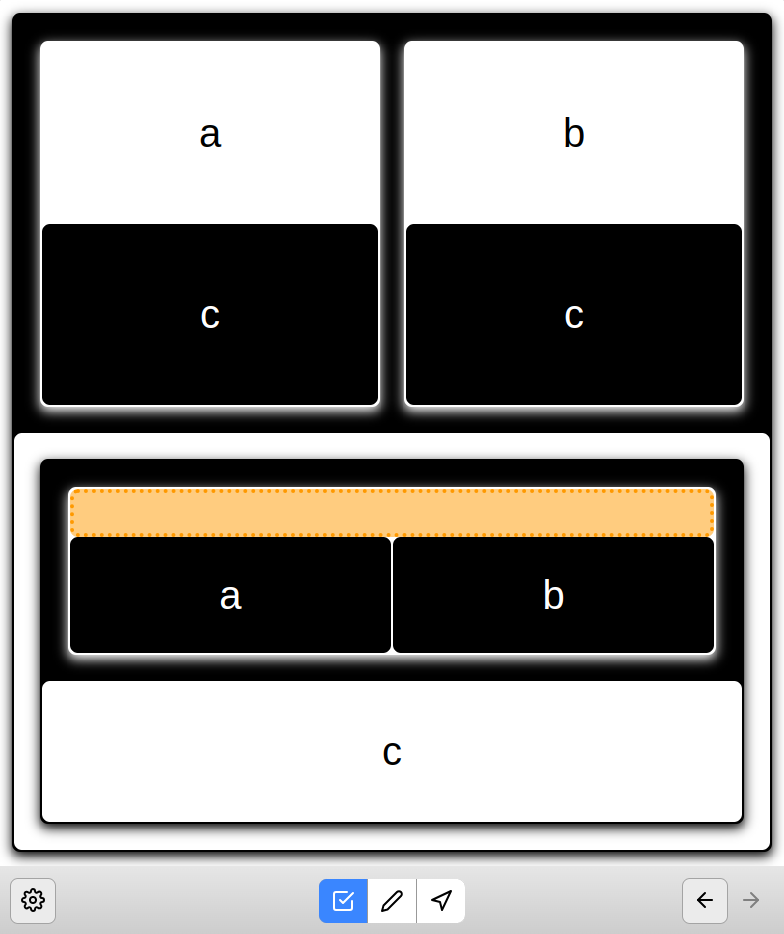
\includegraphics[width=0.7\textwidth]{flower-prover-proof-mode}
  \hspace{1em}
  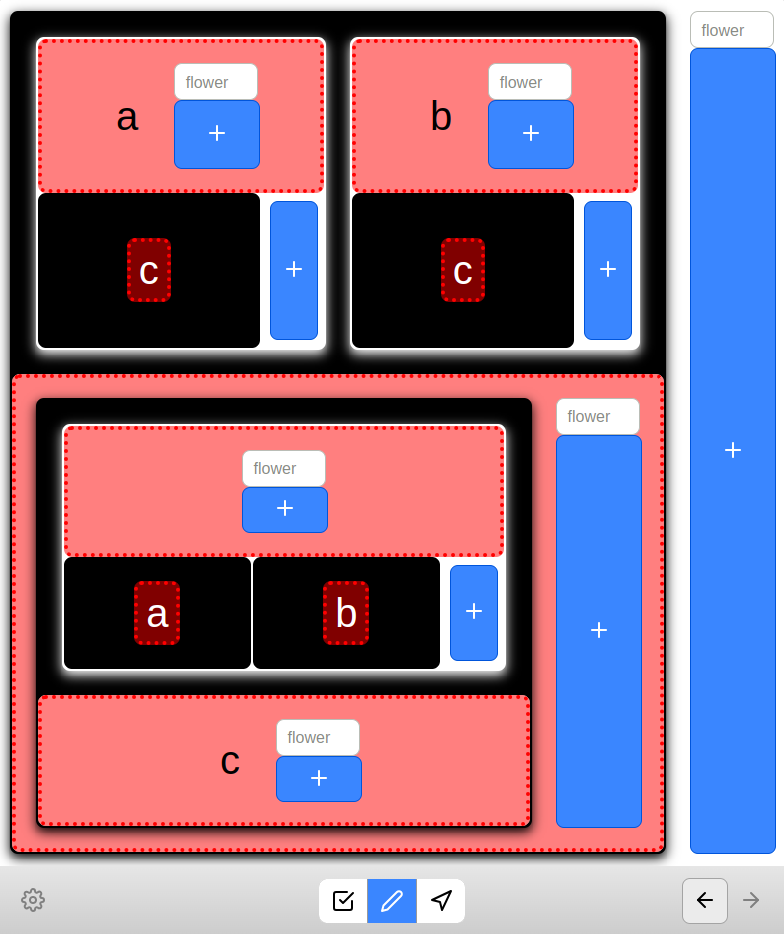
\includegraphics[width=0.7\textwidth]{flower-prover-edit-mode}
  \caption{Proof mode (left) and Edit mode (right) of the Flower Prover}
  \labfig{flowers-prover-modes}
\end{figure*}

\paragraph{Modal interface}

The Flower Prover is organized in two main \emph{modes} of interaction,
providing different sets of available actions to the user\sidenote{Another
example of modal interface is the popular text editor \texttt{vim}, with its
\emph{normal} mode for high-level manipulation of text through commands and
macros, and its \emph{edit} mode for low-level insertion and deletion of
characters.}:
\begin{itemize}
  \item[\textbf{Proof mode}] \todo{TODO}
  \item[\textbf{Edit mode}] \todo{TODO}
\end{itemize}
At any point during a proof, the user can switch between the two modes by
clicking on the corresponding button in the \emph{mode selection bar}, located
at the bottom of the screen (\reffig{flowers-prover-modes}): the proof and edit
modes are mapped respectively to the left button with a checkmark icon, and the
middle button with a pencil icon.

\paragraph{Proof mode}

\todo{Describe every action}
\todo{Example of proof trace with screenshots}

\paragraph{Edit mode}

\todo{Describe every action}

\paragraph{Navigation mode}

The reader might have noticed that there is a third, right button with a
navigation icon in the mode selection bar. It can be used to enter
\emph{navigation mode}, the last mode of interaction that we intend to implement
in the future. The idea is that on real-life goals, both the size and level of
nesting of flowers will quickly render the interface unusable, both for
reading/understanding the content and structure of goals, and manipulating them
through pointing.

The purpose of the navigation mode is then to enable the user to \emph{focus} on
a specific subgoal, by simply clicking on the corresponding nested flower. This
would make the subgoal take up the whole screen, hiding the outer context from
view. Dually, it should also be possible to unfocus a previously focused subgoal
--- e.g. by clicking again, so that the full tree structure of the goal can be
freely navigated.

This way of navigating tree structures represented as nested areas is typical of
\emph{zoomable user interfaces} or ZUI, a strand of GUI that has been developed
by many pioneers in the field of human-computer interaction such as Ivan
Sutherland in its Sketchpad system \sidecite{10.1145/800265.810742}, and Alan
Kay in its Smalltalk system \sidecite{goldberg_smalltalk-72_1976}.

\paragraph{Automation}

\todo{ Describe our current automation as a simple fixpoint applying all the
  applicable actions according to a set of rules. Thus the user could tune the
  level of automation by customizing the set of rules.}

\todo{ Possibility to apply automation systematically after each action, or
  manually by clicking on a button.}

\todo{ Proof trace for the same goal as before, but with default automation
  turned on.}

\todo{ Idea of reducing a proof to a set of DnD pollinations + Case reasoning
with \rsf{srep}. }

\paragraph{Theories and goals}

In the so-called ``proof view'' or ``goal view'' of modern proof assistants like
Coq and Lean, there is no distinction between local and global contexts: a
subgoal will inherit automatically every hypothesis from its parent subgoals,
which are flattened into a big unstructured list. To recreate this distinction
and reduce the size of goals to a manageable level, the only interface mechanism
offered to the user is to exit interactive proof mode, and outsource chunks of
the local context as additional global lemmas and definitions in the current
theory file.

Thus the user has to juggle between two different interfaces that manipulate two
distinct data structures: a traditional text editor for modifying
\emph{theories}, and an IDE for writing and executing proof scripts that modify
\emph{goals}, themselves visualized in a separate proof view. This results in a
duplication of means to achieve essentially the same things: for instance,
reordering two lemmas will require to cut and paste one of them in the theory
file, while reordering two hypotheses will require the use of a dedicated
\texttt{move} tactic. Other examples can be found for renaming definitions,
applying lemmas, constructing functions, etc.

Crucially, the two interfaces cannot communicate straightforwardly with
eachother. In fact, communication is completely one-way: the user can only
invoke definitions and lemmas from the theory in her proof script, by referring
to their names.

\paragraph{Statements and proofs}

Our above example targets imperative tactic languages, but the argument equally
applies to more declarative languages like Isar in Isabelle: the point is that
the \emph{proof} language, be it imperative or declarative, is separated both
conceptually and through its available means of interaction from the language of
\emph{statements} used to build theories. And this separation between proofs and
statements is a natural one that is hard to question, since it is rooted in what
is arguably the most important inspiration of formal logic, and also the form in
which informal mathematics present themselves: \emph{natural language}. Indeed,
symbolic formulas reproduce the grammatical structure of sentences expressing
logical propositions, and proofs reproduce the inferential structure of
arguments built from sequences of sentences.

\paragraph{Diagrams}

However, there is an increasing number of areas in mathematics --- the most
prominent one being category theory --- where the heart of a proof lies in the
dynamical construction of a \emph{diagram} capturing the structure of interest
in given mathematical objects. The natural language proof text is often just a
mean to explicit the meaning or intuition behind the diagrammatic manipulations,
or simply a retranscription of the commentary that the mathematician would give
when unfolding the construction on a blackboard. If one views logic as one
particular type of mathematical reasoning --- albeit one that is omnipresent in
all branches of mathematics, then it is only natural to expect that some
diagrammatic system should exist for it, that can express in the most natural
way most (if not all) logical arguments. This is the \emph{iconicity} thesis of
Peirce, and what we are aiming for with the Flower Prover.

\paragraph{Context navigation}

After this little conceptual \textit{aparté}, let us come back to the problem of
managing contexts in proofs. In the Flower Prover, the \emph{local} context is
naturally represented as \emph{everything that is displayed on-screen}. This
includes hypotheses that are available from pistils at various levels, but also
potentially alternative goals (adjacent petals) and further subgoals (positively
nested flowers). Then rather than being segregated in a separate interface (the
text buffer of the theory), the \emph{global} context is simply the
\emph{entire} goal. In fact, there is no reason anymore to make a terminological
distinction between goals and theories: a goal is just a theory that has yet to
be justified, which can itself be identified with a partial proof (or a ``proof
term with holes'' in type theory)\sidenote{We will come back to this idea of
merging proofs and statements in the same data structure in the conclusion, when
discussing \emph{development calculi}. Note however that it is already at the
heart of \emph{dependent} type theory, where terms can freely occur inside
types.}.

It would still be useful to be able to aggregate automatically the set of all
lemmas and definitions (i.e. hypotheses) available in a focused subgoal
$\Phi\select{\phi}$, so that the user does not need to navigate up and down the
goal tree all the time. This can be done with the help of the pollination
relation (\refdef{pollination}), by taking the union $\Psi =
\compr{\psi}{\chyp{\psi}{\Phi\hole}}$.

In terms of UI, we could then add a ``shelf'' displayed in all interaction
modes, that exposes the global context $\Psi$ of the current focus $\Phi\hole$.
We anticipate only two kinds of interaction with the shelf:
\begin{itemize}
  \item[\textbf{Pollination}] \todo{TODO}
  \item[\textbf{Jump to definition}] \todo{TODO}
\end{itemize}

Since the shelf might contain \emph{a lot} of hypotheses, it will be important
to provide efficient ways to \emph{filter} or \emph{search} through its content.
We imagine three main ways to do so:
\begin{itemize}
  \item[\textbf{By name}] the user can type the \emph{name} of a hypothesis in a
  search bar. This implies that flowers have the ability to be named by the
  user.
  \item[\textbf{By structure}] the user can specify a \emph{pattern} that must
  be satisfied by all hypotheses in the shelf. A pattern is just a flower that
  contains pattern variables, which can match any flower. Thus patterns might be
  built with the same tools offered in Edit mode.
  \item[\textbf{By selection}] the user can select subterms of the goal, and
  then ask the system to display only hypotheses that can \emph{interact} with
  these subterms. Here we imagine something along the lines of what we did for
  Actema (\refsec{funcs}).
\end{itemize}

\begin{remark}
  The first two types of filtering are already available in most proof
  assistants, i.e. the \texttt{Search} command of Coq.
\end{remark}

% \section{Towards a Curry-Howard correspondence}\labsec{flowers-curryhoward}

% \todo{Write simulation of modus ponens $A \land (A \limp B) \limp B$}

% Let us give an example of how to \emph{simulate} a rule from natural deduction
% in the flower calculus. Rather than reducing the bouquet associated to a formula
% to the empty bouquet, we want to reduce the bouquet associated to the conclusion
% of the rule into the bouquet associated to its premisses. \reffig{flowers-mp}
% shows how to proceed in the case of the elimination rule for $\limp$, or
% \emph{modus ponens}. A crucial step is the use of the \rsf{grow} rule, which
% allows to create a positive occurrence of $A$ out of thin air. This is the main
% source of non-analyticity in the flower calculus, in the sense of the
% \emph{subformula property} of Gentzen. Although we showed in
% \refsec{Completeness} that the \rsf{grow} rule is admissible, it was for the
% relation of \emph{provability} (\refdef{flowers-proof}). Here to simulate modus
% ponens we rely on \emph{derivability}, and thus need this rule.

% The derivation of \reffig{flowers-mp} also makes clear that it is the positive
% $A$ that justifies the negative one with the \rsf{poll{\ua}} rule, and not
% the other way around. Indeed, the presence of the pistil around the negative $A$
% makes it deeper than the positive $A$, preventing the \rsf{poll{\ua}} rule
% from being applicable in the other direction. This is a manifestation of the
% inherent dissymmetry in \emph{proof substitution}: the erasure of the negative
% $A$ can be interpreted as the operation $\subst{\pi_B}{\pi_A}{x}$, which
% substitutes every occurrence of the associated hypothesis $x$ in the proof
% $\pi_B$ of $B$ by the proof $\pi_A$ of the positive $A$.
% \todo{ Elaborate further on this computational aspect of EG. }
% \todo{ Investigate the ``scientific'' iteration rule of Peirce as a means to
% avoid the need for a computational interpretation of the \rsf{epis} rule. }


\section{Conclusion}\labsec{Conclusion}

\subsection{Related works}

\paragraph{Intuitionistic EG}
  
\begin{marginfigure}
  \begin{mathpar}
    \R[\rsf{iter}]
      {\flower{\gamma}{\delta \sep \Delta}}
      {\flower{\gamma}{\delta \sep \delta \sep \Delta}}
    \and
    \R[\rsf{deit}]
      {\flower{\gamma}{\delta \sep \delta \sep \Delta}}
      {\flower{\gamma}{\delta \sep \Delta}}
  \end{mathpar}
  \caption{(De)iteration rules for petals}
  \labfig{flowers-deit-petals}
\end{marginfigure}

In the original IEG system of Oostra, the \rsf{srep} rule is replaced by an
extended (de)iteration rule, that allows to duplicate/merge not only identical
flowers, but also identical \emph{petals}, under the condition that they are
attached to the same pistil\sidenote{``Cualquier lazo puede iterarse adherido
\emph{al mismo corte}'' \cite[p.~46]{oostra_graficos_2010}.} (rules \rsf{iter}
and \rsf{deit} in \reffig{flowers-deit-petals}). Thus in a sense, (de)iteration
on petals is not as \emph{deep} as on whole flowers, where the two identical
flowers can be separated by an arbitrary number of layers; which might seem like
an arbitrary restriction. A posteriori, we rationalize this choice by seeing it
as an attempt to stay close to the original system \sys{Alpha} of Peirce. In
particular, (de)iteration on petals is compatible with the quest for
\emph{illative atomicity}, where all rules should be expressed in terms of
insertions and omissions (\refsec{atomicity}); while the \rsf{srep} rule is not.
In our case, this is justified by our quest for an \emph{invertible} calculus
(natural fragment): indeed to simulate \rsf{srep} with petal (de)iteration, one
also needs the non-invertible $\Culture$-rule \rsf{crop} (as well as the
$\Culture$-rule \rsf{epis{\da}}), as illustrated by the \rsf{srep}-free proof of
\reffig{flowers-srep-free}.

\begin{figure}
  \begin{mathpar}
  \prftree[r][d]{\rsf{poll{\ua}}}
  {\prftree[r][d]{\rsf{poll{\da}}}
  {\prftree[r][d]{\rsf{crop}}
  {\prftree[r]{\rsf{iter}}
  {\prftree[r][d]{\rsf{epis{\da}}}
  {\prftree[r]{\rsf{poll{\da}}}
  {\prftree[r]{\rsf{epet}}
  {}
  {\flower{(\flower{a}{c}),(\flower{b}{c}),c}{\garden{}{}}}}
  {\flower{(\flower{a}{c}),(\flower{b}{c}),c}{c}}}
  {\flower{(\flower{a}{c}),(\flower{b}{c}),(\flower{}{(\flower{}{c})})}{c}}}
  {\flower{(\flower{a}{c}),(\flower{b}{c}),(\flower{}{(\flower{}{c}) \sep (\flower{}{c})})}{c}}}
  {\flower{(\flower{a}{c}),(\flower{b}{c}),(\flower{}{(\flower{}{c}), a \sep (\flower{}{c}), b})}{c}}}
  {\flower{(\flower{a}{c}),(\flower{b}{c}),(\flower{}{(\flower{a}{c}), a \sep (\flower{b}{c}), b})}{c}}}
  {\flower{(\flower{a}{c}),(\flower{b}{c}),(\flower{}{a \sep b})}{c}}
\end{mathpar}
% \begin{mathpar}
%   \prftree[r][d]{\rsf{poll{\ua}}}
%   {\prftree[r][d]{\rsf{poll{\da}}}
%   {\prftree[r][d]{\rsf{crop}}
%   {\prftree[r]{\rsf{iter}}
%   {\prftree[r][d]{\rsf{srep}}
%   {\prftree[r]{\rsf{poll{\da}}}
%   {\prftree[r][d]{\rsf{epet}}
%   {}
%   {\flower{(\flower{a}{c}),(\flower{b}{c})}{(\flower{}{(\flower{c}{\garden{}{}})})}}}
%   {\flower{(\flower{a}{c}),(\flower{b}{c})}{(\flower{}{(\flower{c}{c})})}}}
%   {\flower{(\flower{a}{c}),(\flower{b}{c}),(\flower{}{(\flower{}{c})})}{c}}}
%   {\flower{(\flower{a}{c}),(\flower{b}{c}),(\flower{}{(\flower{}{c}) \sep (\flower{}{c})})}{c}}}
%   {\flower{(\flower{a}{c}),(\flower{b}{c}),(\flower{}{(\flower{}{c}), a \sep (\flower{}{c}), b})}{c}}}
%   {\flower{(\flower{a}{c}),(\flower{b}{c}),(\flower{}{(\flower{a}{c}), a \sep (\flower{b}{c}), b})}{c}}}
%   {\flower{(\flower{a}{c}),(\flower{b}{c}),(\flower{}{a \sep b})}{c}}
% \end{mathpar}
  \caption{Simulating the \rsf{srep} rule by iterating petals}
  \labfig{flowers-srep-free}
\end{figure}

\paragraph{Focusing}

There is a formal connection between the \rsf{poll{\ua}} rule of the flower
calculus, and the \emph{absorption} rule $[\mathbf{A}]$ of the dyadic system
$\Sigma_2$ of Andreoli, that handles the focusing behavior of exponentials in
linear logic \sidecite{andreoli1992}. Indeed, both rules duplicate a formula
available in the (non-linear) context of the sequent/location where the rule is
applied, in order to enable further usage of the formula at said location. While
the absorption rule removes the need for permutation-equivalences between proofs
involving the \emph{contraction} rule, the identity rule $[I]$ of $\Sigma_2$
removes the need for the \emph{weakening} rule by discarding the non-linear
context in one go, just as the \rsf{epet} rule of the flower calculus renders
the \rsf{crop} rule admissible.

Sonia Marin has noticed the connection between \emph{bipoles} in focused proofs,
and the class of geometric/coherent formulas, where the former are seen as a
generalization of the latter \sidecite{marin_axioms_2022}. This is to be related
to our own identification of $n$-ary scrolls/flowers as a recursive
generalization of coherent formulas at the end of \refsec{IEG}.

Two years earlier, Brock-Nannestad and Ilik had already made some implicit
connections between focused proofs and coherent formulas, through their
\emph{exponential normal form} for intuitionistic formulas based on Tarski's
highschool identities \sidecite{brock-nannestad_intuitionistic_2019}. Quite
remarkably, first-order formulas in their exponential normal form have the exact
same structure as flowers
\cite[Definition~4.2]{brock-nannestad_intuitionistic_2019}. However, the sequent
calculus \sys{HS} based on them makes the tradeoff opposite to that of the
natural fragment $\Nature$ of the flower calculus: every inference rule is
\emph{non}-invertible, but the calculus is contraction-free. One advantage of
this tradeoff is that they can easily show termination of proof search, while we
have not found a terminating procedure yet for the flower calculus. The authors
also mention that \sys{HS} could be turned into a deep inference calculus in the
style of \sys{G4ip}\sidenote{This is just another name for the system \sys{LJT}
of Dyckhoff already mentioned in \refch{bubbles-symm}.}.

\paragraph{Development calculi}

In \refsec{flowers-prover}, we have seen how the rules of the flower calculus
can be understood as a set of (graphical) tactics for building partial proofs
interactively. In Chapter 3 of his thesis \sidecite{ayers_thesis}, Ayers calls
such systems \emph{development calculi}. In particular, he presents his own
development calculus inspired by McBride's OLEG system
\sidecite{mcbride_dependently_2000} and G\&G's prover
\sidecite{ganesalingam_fully_2017} called the \texttt{Box} calculus, where both
goals and partial proofs are represented by the same \texttt{Box} datastructure.
Once again, \texttt{Box}es seem to share a very similar structure with flowers,
which was here motivated by the need to avoid backtracking by having the ability
to maintain a disjunction of goals with so-called \emph{disjunctive pairs},
corresponding to the petals of flowers. The main difference is that the
\texttt{Box} calculus is based on dependent type theory instead of first-order
logic: this allows to store the partial proof terms inside of the \texttt{Box}es
themselves, while this information is lost during the construction of flowers
(but might be reconstructed from the sequence of graphical actions and the
initial goal).

Ayers also mentions the category-theoretical treatment of development calculi by
Sterling and Harper \sidecite{sterling_algebraic_2017}, that abstracts from any
particular type of judgment. Thus it might be possible to fit the flower
calculus into this framework, by identifying the set of flowers $\flowers$ as a
category of \emph{nested judgments}\sidenote{Nested judgments are already
considered in some recent categorical semantics of type theory, and in
particular those in Sterling's thesis \cite{Sterling2022}. See also
\cite{huang2023synthetic} for a (technical) introduction to the subject.}.

\paragraph{Subformula linking}

Our notion of \emph{vehicle} (\refdef{vehicle}) takes its terminology from
Girard, who started giving this name to the set of axiom links of a proof
structure in his transcendental syntax\sidenote{Also, it conveys nicely the idea
that the vehicle is the fundamental structure that \emph{drives} the proof
search algorithm.} \sidecite{girard_2017}. But the idea of connecting dual
occurrences of atoms, and thus forming a graph with an associated adjacency
matrix whose structure can be exploited in proof search, really dates back to
the \emph{connection method} developed independently by Bibel and Andrews in the
1970s \sidecite{Bibel:2009}. Otten and Kreitz have adapted the connection method
to intuitionistic logic \sidecite{10.1007/3-540-59338-1_32}, stating that it is
especially well-suited in an interactive theorem proving environment. Thus it
might be instructive to learn from their proof search algorithm to fix ours.

In fact all proof search procedures designed in this thesis, whether for bubble
calculi (\refsubsec{bubbles-search}) or the flower calculus
(\refsec{flowers-search}), rest on the fundamental observation coming from the
subformula linking methodology of Chaudhuri \sidecite{Chaudhuri2013}, that the
construction of proofs in deep inference systems can be driven efficiently and
incrementally by the connection of dual atoms. With its pollination rules, the
flower calculus allows for a particularly elegant implementation of subformula
linking that abstracts away from the syntactic bureaucracy of symbolic
connectives, as witnessed by the pollination phase of our search procedure. In
\refsubsec{bubbles-search}, we sketched some ideas that blur the frontier
between automated and interactive proof search, notably with the so-called
\emph{rule of thumb} which is another manifestation of subformula linking. This
integration of automated and interactive aspects is also at work in the Flower
Prover, and it would be interesting to investigate further how to incorporate
our drag-and-drop proof tactic (\refch{pba}), but also other symbolic
manipulation techniques introduced in the first part of this thesis, into the
iconic framework of the Flower Prover.

\paragraph{Analyticity}

We have not discussed the rationale behind our notion of analyticity, be it
historical or formal arguments explaining its origins, motivations and
consequences. In a recent article \sidecite{bruscoli_analyticity_2019}, Bruscoli
and Guglielmi propose such a detailed discussion around a precise and generic
definition of analyticity for deep inference proof systems (especially the
calculus of structures), which at a glance seems to encompass our own
definition. It would be interesting to study more deeply their work, and related
parts of the deep inference literature concerned with analyticity and its
applications to efficient proof search procedures
\sidecite{kahramanogullari_reducing_2006}\sidecite{lmcs:1089}\sidecite{10.1145/2003476.2003501}\sidecite{chaudhuri:hal-00772420}\sidecite{10.1007/978-3-662-49630-5_23}.

\subsection{Future works}

\paragraph{Metatheory}

In \refsec{Calculus}, we already mentioned the variant $\Nature \setminus
\{\rsf{epis}\} \cup \{\rsf{crep}\}$ of the natural fragment, that we conjecture
to enjoy both soundness, completeness and a deduction theorem. But these last
two results shall prove particularly harder to prove, and we currently have very
few insights into how to extend the proofs of this chapter to this setting.
Also, this is not withstanding the fact that we do not really see any practical
applications for such results as of yet. Our initial motivation was to show the
admissibility of the \rsf{epis} rule, because it never appears in concrete
proofs. But if this requires adding the \rsf{crep} rule instead, then it greatly
reduces the pratical interest of the whole endeavor, since the \rsf{crep} rule
does not look particularly well-suited to either automated or interactive
theorem proving.

\paragraph{Automated proof search}

We shall investigate the current sources of non-termination and incompleteness
for our \refproc{life} proof search procedure, through further testing on the
ILTP dataset. If we succeed in passing all tests, the natural continuation will
be to provide formal proofs of termination and completeness. A follow-up
direction would be to extend our algorithm to the first-order setting by adding
heuristics for handling sprinklers, thus losing completeness.

Another direction of research would consist in comparing our algorithm to
existing search procedures for EG, in particular one that was originally
developed by Peirce, and described by Oostra in \sidecite{oostra_advances_2022}.

\paragraph{Flower Prover}

Implement the navigation mode in the Flower Prover, and
design GUI mechanisms that support relational reasoning with sprinklers, based
on the rules \rsf{ipis}, \rsf{ipet} and \rsf{apis}, \rsf{apet}.

\paragraph{Curry Howard}

We have begun to sketch some ideas for a Curry-Howard correspondence, where
flowers and actions (rules) for justifying them are identified respectively with
\emph{normal} and \emph{neutral} terms of the simply-typed $\lambda$-calculus.
For instance, the computational counterpart of the rule \rsf{poll{\da}} in
pistils would be a kind of \emph{function application} expressed by the
following \rsf{app} rule, which is highly reminiscent of the instantiation rule
\rsf{ipis}:
$$
\R[\rsf{app}]
  {\Xi\select{t~u : (\flower{\subst{\Phi}{u}{x}}{\subst{\Delta}{u}{x}})}}
  {\Xi\select{t : (\flower{\Phi, x : \phi}{\Delta})}}
$$
Given a flower $\phi$ and a neutral term $t$, i.e. an $n$-ary function
application of the form $x~t_1 \ldots t_n$, the expression $t : \phi$ is a
\emph{term annotation}, that should be read in context as ``this occurrence of
$\phi$ is justified by $t$''. Interestingly, $\phi$ itself may contain term
annotations, mimicking the fact that normal and neutral terms can be defined by
mutual recursion. Then in the \rsf{app} rule, we do not just erase the formula
$\phi$ as in the \rsf{poll{\da}} rule, but also keep track of the flow of
information by appending the argument $u$ to the justification $t$ (where
$\chyp{(u : \phi)}{\Xi\hole}$), and substituting $u$ to every occurrence of the
hypothetical justification $x$ of $\phi$ in $\Phi$ and $\Delta$.

As of now the syntax of annotated flowers is not yet stable, and it is unclear
what would be the computational interpretation of flowers with $n \not= 1$
petals. In particular for disjunctive flowers ($n > 1$), it seems that we are
closer to a notion of non-deterministic or parallel computation, than to the
usual branching computation of sum or inductive types.

If our intuition is right, then the fact that flowers correspond to (normal)
$\lambda$-terms would embody syntactically a recent motto from Miquel stemming
from his study of the foundations of forcing and realizability in implicative
algebras, where ``elements can be seen both as truth values and as (generalized)
realizers, thus \textbf{blurring the frontier between proofs and
types}''\sidenote{Another recent, related incarnation of this phenomenon is the
correspondence uncovered by Haydon between a linear version of EG already
appearing in Peirce's writings, and the proof nets of Girard for linear logic
\cite{haydon_eg_pn}.} \sidecite{miquel_implicative_2020}. Or as he put it in a
recent talk \cite{miquel_implicative_topos_2022}, we get the ultimate
Curry-Howard identification:
$$
\text{\textbf{Realizer}} = \text{\textbf{Program}} = \text{\textbf{Formula}} = \text{\textbf{Type}}
$$
This could also form the basis for further studies on the connections between EG
and (dependent) type theory, and ultimately lead to a tight integration of the
Flower Prover with proof assistants based on the latter such as Coq, Lean and
Agda. Existing explorations of the links between type theory and deep inference
include, in historical order:
\begin{itemize}
  \item a first attempt by Brünnler and McKinnley to devise a Curry-Howard
  correspondence for a simple intuitionistic deep inference calculus with
  conjunction and implication \sidecite{cervesato_algorithmic_2008};
  \item the thesis of Nicolas Guenot, and more precisely the part on "Nested
  Proofs as Programs" where he gives a correspondence between simply-typed
  $\lambda$-calculi with explicit substitutions at one end, and calculi of
  structures (Chapter 6) and nested sequent calculi (Chapter 5) for the
  implicational fragment of intuitionistic logic at the other end
  \cite{guenot_nested_2013};
  \item the atomic $\lambda$-calculus, a simply-typed $\lambda$-calculus with
  explicit sharing that has a Curry-Howard correspondence with proofs in the
  formalism of \emph{open deduction} \sidecite{gundersen_atomic_2013};
  \item a type system for interaction nets based on a calculus of structures for
  Multiplicative Exponential Linear Logic \sidecite{gimenez_structure_2013};
  \item the thesis of Fanny He, that explores a classical variant of the atomic
  $\lambda$-calculus based on Saurin's $\Lambda\mu$-calculus
  \sidecite{he_fanny_thesis};
  \item the \emph{spinal} atomic $\lambda$-calculus, an extension and
  improvement on the atomic $\lambda$-calculus based on a computational
  interpretation of the \emph{switch} rule \sidecite{goubault-larrecq_spinal_2020};
  \item the \emph{collection calculus} that subsumes resource,
  intersection-typed and simply-typed $\lambda$-calculi, with a type system
  again in open deduction \sidecite{guerrieri_deep_2021};
  \item Ongoing research by Kaustuv Chaudhuri to extend subformula linking to
  dependent type theory\sidenote{Private communication.}.
\end{itemize}
The work of Guenot on computational interpretations of nested sequent calculi
seems closest to the syntax of flowers. Indeed, nested sequents are variadic by
nature, and his version of nested sequents in particular exploits the
possibility to have \emph{negative} occurrences of sequents. Combined with the
dependently-typed \texttt{Box}es of Ayers mentioned earlier (which cannot be
nested negatively), this should provide great insights for the powerful,
dependently-typed version of the flower calculus that we seek for.

\subsection{Theory vs. Practice}

Finally, it should be noted that Peirce did not think of EG as a calculus that
could aid in performing reasoning \emph{per se}, but rather as a tool for
analysing the finer structure of logical endeavor
\cite[pp.~110-111]{Roberts+1973}:
\begin{quote}
  [...] the purpose which the system was designed to fulfill was ``to enable us
to separate reasoning into its smallest steps so that each one may be examined
by itself'' (Ms 455, p.2). The aim was not to facilitate reasoning, but to
facilitate the study of reasoning.
\end{quote}

The various achievements presented in this chapter incite us to depart from this
conception. Indeed, our particular viewpoint on the illative transformations,
that emphasizes goal-reduction through invertible and analytic rules, enabled us
to design a novel and promising type of graphical interface for interactive
proof building, which integrates easily and elegantly some (limited) forms of
automation. This was also made possible by the use of variables instead of lines
of identity, trading a heavy graphical apparatus with local inference rules for
a simple, well-known textual syntax with complex (but automated) global dynamics
in the form of substitutions. Hence we believe the \emph{opposite}, that EG
\emph{can} form the basis for an ergonomic calculus of logical deduction, in
addition to being a powerful tool for meta-logical analysis.